% !TeX program = xelatex
% =============================================================================
%  DỰ ÁN TỐT NGHIỆP — BÁO CÁO CHÍNH (BẢN OUTLINE SỰ KIỆN)
%  Đề tài: Phân tích Hiệu suất và Dự báo Sản lượng Hệ thống Điện Mặt Trời
%  Nhóm: The Outliers
%  Trường: Cao đẳng FPT Polytechnic — Chuyên ngành Phân tích Dữ liệu
% =============================================================================

\documentclass[12pt, a4paper]{report}

% ======================== PACKAGES ==========================================
\usepackage{fontspec}
\usepackage[vietnamese]{babel}

% Ngan ch?n t? d?ng g?ch n?i t? (hyphenation) cu?i d�ng
\hyphenpenalty=10000
\exhyphenpenalty=10000
\tolerance=10000
\emergencystretch=3em

\usepackage{geometry}
% footskip mac dinh 30pt, ma tai lieu dung gian dong 1,5 nen moi dong cao ~21,75pt:
% chan trang chi cach chan chu khoang 8pt, trang nao day chu la cham vao dong 'Du an
% Tot nghiep'. Ha chan trang xuong 1,5cm de co khoang ho, le trai/phai/tren giu nguyen.
\geometry{top=2.5cm, bottom=2.5cm, left=3cm, right=2cm, footskip=1.5cm}
% ======================== CẤU HÌNH CODE PYTHON (MUTED STYLE) ==============================
\usepackage{listings}
\usepackage{xcolor} % Bắt buộc phải có để dùng \definecolor

% Định nghĩa lại bảng màu dịu, ít sặc sỡ và chuyên nghiệp hơn
\definecolor{mutedgreen}{rgb}{0.2,0.5,0.3}    % Màu xanh lá trầm cho comment
\definecolor{mutedblue}{rgb}{0.15,0.35,0.6}   % Màu xanh dương dịu cho keywords thay cho magenta
\definecolor{mutedgray}{rgb}{0.45,0.45,0.45}  % Màu xám cho số dòng
\definecolor{mutedpurple}{rgb}{0.45,0.2,0.55} % Màu tím trầm cho strings thay cho codepurple
\definecolor{softbackground}{rgb}{0.98,0.98,0.98} % Màu nền xám trắng siêu nhẹ tránh mỏi mắt
\definecolor{bordergray}{rgb}{0.85,0.85,0.85}  % Màu viền xám nhạt

\lstdefinestyle{pythonstyle}{
    backgroundcolor   = \color{softbackground},
    commentstyle      = \color{mutedgreen}\itshape, % Comment chữ nghiêng xanh trầm
    keywordstyle      = \color{mutedblue}\bfseries, % Keyword chữ đậm xanh dịu
    numberstyle       = \tiny\color{mutedgray},
    stringstyle       = \color{mutedpurple},
    basicstyle        = \ttfamily\small\color{black}, % Chữ code mặc định màu đen thuần
    breakatwhitespace = false,
    breaklines        = true,
    captionpos        = t, 
    keepspaces        = true,
    numbers           = left,
    numbersep         = 5pt,
    showspaces        = false,
    showstringspaces  = false,
    showtabs          = false,
    tabsize           = 4,
    frame             = single,
    rulecolor         = \color{bordergray}, % Viền mảnh màu xám nhạt tinh tế
    extendedchars     = true,
    }
\lstset{style=pythonstyle}

% Font - Arial (Sans-Serif, fully supports Vietnamese on Windows/XeLaTeX)`r`n\setmainfont{TeX Gyre Termes}
\setmonofont{TeX Gyre Cursor}

% Header / Footer
\usepackage{fancyhdr}
\usepackage{lastpage}

% Hyperlinks & Bookmarks
\usepackage{hyperref}
\hypersetup{
    colorlinks  = true,
    linkcolor   = black,
    citecolor   = blue,
    filecolor   = magenta,
    urlcolor    = blue,
    pdftitle    = {Dự án Tốt nghiệp - Phân tích Hiệu suất và Dự báo Sản lượng Hệ thống Điện Mặt Trời},
    pdfauthor   = {The Outliers - FPT Polytechnic},
    bookmarksnumbered = true,
}

% Toán, ký hiệu
\usepackage{amsmath, amssymb}

% Danh sách
\usepackage{enumitem}
\usepackage{array}

% Bảng biểu
\usepackage{booktabs}
\usepackage{tabularx}
\usepackage{longtable}
\usepackage{multirow}
\usepackage{array}

% Hình ảnh
\usepackage{graphicx}
\usepackage{float}
\usepackage{caption}
\usepackage{subcaption}
% placeins cho \FloatBarrier: chan khong cho hinh/bang cua mot muc troi sang muc sau.
% Khong dung tuy chon [section] vi no ap cho CA tai lieu; o day chi dat rao thu cong
% truoc tung \section cua chuong Hoc may, khong dung toi bo cuc cac chuong khac.
\usepackage{placeins}
% \needspace{n\baselineskip}: neu cuoi trang con it hon n dong thi sang trang moi, con du
% cho thi khong lam gi. Dung de mot doan ngan va khoi ket xuat di theo no khong bi cat doi
% qua hai trang. Khac \filbreak o cho \filbreak luon uu tien ngat, con \needspace chi ngat
% khi that su thieu cho - nho vay khong de lai trang trong. Dinh nghia lay dung tu goi
% needspace (goi nay khong co san trong ban TeX o may nay, chi phat hanh dang .dtx).
\makeatletter
\newcommand{\needspace}[1]{%
  \begingroup
    \setlength{\dimen@}{#1}%
    \vskip\z@\@plus\dimen@
    \penalty -100\vskip\z@\@plus -\dimen@
    \vskip\dimen@
    \penalty 9999\vskip -\dimen@
    \vskip\z@skip
  \endgroup}
\makeatother
% Chu thich hinh/bang KHONG can deu hai ben. Chu thich hay chua ten tep dai khong ngat
% dong duoc; ep can deu thi TeX phai gian khoang trang cua dong tren ra toi da, thanh ra
% 'chu nam xa nhau'. Bo can deu o rieng chu thich la het hien tuong do, than bai van
% can deu binh thuong. Chu thich mot dong van can giua nhu cu.
\captionsetup{justification=raggedright}

% Màu sắc & Code
\usepackage{xcolor}
\usepackage{listings}

% Kẻ khung trang bìa
\usepackage{tikz}

% Danh mục hình, bảng
\usepackage[titles]{tocloft}

% Indent đoạn đầu
\usepackage{indentfirst}
\setlength{\parindent}{1cm}
\setlength{\parskip}{6pt}

% Line spacing
\usepackage{setspace}
\onehalfspacing
\setlength{\headheight}{33pt}

% ======================== CẤU HÌNH CODE PYTHON ==============================
\definecolor{codegreen}{rgb}{0,0.6,0}
\definecolor{codegray}{rgb}{0.5,0.5,0.5}
\definecolor{codepurple}{rgb}{0.58,0,0.82}
\definecolor{backcolour}{rgb}{0.96,0.96,0.94}
\definecolor{fptorange}{RGB}{245,130,32}

\lstdefinestyle{pythonstyle}{
    backgroundcolor   = \color{backcolour},
    commentstyle      = \color{codegreen},
    keywordstyle      = \color{magenta},
    numberstyle       = \tiny\color{codegray},
    stringstyle       = \color{codepurple},
    basicstyle        = \ttfamily\small,
    breakatwhitespace = false,
    breaklines        = true,
    captionpos        = r,
    keepspaces        = true,
    numbers           = left,
    numbersep         = 5pt,
    showspaces        = false,
    showstringspaces  = false,
    showtabs          = false,
    tabsize           = 4,
    frame             = single,
    rulecolor         = \color{codegray},
}
\lstset{style=pythonstyle}

% --- CẤU HÌNH KHOẢNG TRỐNG TIÊU ĐỀ CHƯƠNG ---
\usepackage{titlesec}
% C? ch? 13pt cho c�c section headers
\titleformat*{\section}{\fontsize{13pt}{15.6pt}\bfseries}
\titleformat*{\subsection}{\fontsize{13pt}{15.6pt}\bfseries}
\titleformat*{\subsubsection}{\fontsize{13pt}{15.6pt}\bfseries}
% Cấu hình cho \chapter và \chapter*
\titleformat{\chapter}[display]
  {\normalfont\huge\bfseries}{}{0pt}{\huge}
\titlespacing*{\chapter}{0pt}{-10pt}{20pt} 
% Tham số: {lề trái}{khoảng trống phía trên}{khoảng trống phía dưới tiêu đề}
% ======================== HEADER / FOOTER ====================================
% Trang nội dung chính (Logo ở header trái, THE OUTLIERS ở header phải)
\fancypagestyle{main}{
    \fancyhf{}
    \fancyhead[L]{\includegraphics[height=1cm]{figures/logo_fpoly.png}}
    \fancyhead[R]{\small THE OUTLIERS}
    \fancyfoot[L]{\small Dự án Tốt nghiệp}
    \fancyfoot[R]{\small Page \thepage\ of \pageref{LastPage}}
    \renewcommand{\headrulewidth}{0.4pt}
    \renewcommand{\footrulewidth}{0.4pt}
}

% Trang đầu chương (plain)
\fancypagestyle{plain}{
    \fancyhf{}
    \fancyfoot[L]{\small Dự án Tốt nghiệp}
    \fancyfoot[R]{\small Page \thepage\ of \pageref{LastPage}}
    \renewcommand{\headrulewidth}{0pt}
    \renewcommand{\footrulewidth}{0.4pt}
}

% Trang mở đầu (roman numbering)
\fancypagestyle{front}{
    \fancyhf{}
    \fancyfoot[L]{\small Dự án Tốt nghiệp}
    \fancyfoot[R]{\small Page \thepage\ of \pageref{LastPage}}
    \renewcommand{\headrulewidth}{0pt}
    \renewcommand{\footrulewidth}{0.4pt}
}

% =============================================================================
%                           BẮT ĐẦU TÀI LIỆU
% =============================================================================

% ── Bo sung cho chuong Hoc may (Section6_body.tex) ──
\usepackage{flafter}   % float khong xuat hien truoc cho duoc nhac toi
\usepackage{microtype}
\usepackage{url}
\newcolumntype{L}[1]{>{\raggedright\arraybackslash}p{#1}}
% \tep: in ten cot/ten tep co dau gach duoi ma khong vo.
% Cho phep NGAT DONG sau '/' va '_' de mot duong dan dai khong bi day nguyen cuc xuong
% dong duoi, vi chinh viec do lam TeX phai gian khoang trang dong tren ra toi da (dong
% 'chu nam xa nhau'). Chu khong doi mot ky tu, chi them cho duoc phep xuong dong; khong
% chen dau gach noi nen doc lai van ra dung ten tep.
% \tep in ten cot/ten tep, giu nguyen dau gach duoi, va CHO PHEP xuong dong sau '/' va '_'.
% Cach lam: \detokenize bien chuoi thanh cac ky tu thuong, roi duyet tung ky tu, gap '/'
% hoac '_' thi chen mot diem ngat rong (\discretionary rong ca ba phan) - tuc chi cho phep
% xuong dong chu KHONG them ky tu nao, doc lai van ra dung ten tep.
%
% Vi sao khong dung \DeclareUrlCommand cua goi url: lenh do doi catcode, dung trong tai lieu
% nay lam vo toan bo cong thuc toan (da thu, 749 loi). Vong lap duoi day khong dong toi
% catcode nen an toan.
%
% Luu y: vong lap doc doi so khong bao gom dau cach, nen \tep{...} KHONG duoc chua dau cach.
% Ba cho tung co dau cach da duoc tach thanh \tep{a}${}={}$\tep{b}.
\makeatletter
\DeclareRobustCommand{\tep}[1]{\texttt{\expandafter\tep@duyet\detokenize{#1}\tep@het}}
\def\tep@het{\tep@het}
\def\tep@duyet#1{%
  \ifx#1\tep@het
  \else
    #1\tep@ngat{#1}\expandafter\tep@duyet
  \fi}
% Dinh nghia voi '_' o catcode 12 cho khop voi ky tu ma \detokenize sinh ra.
{\catcode`\_=12 \gdef\tep@ngat#1{\if#1/\discretionary{}{}{}\else\if#1_\discretionary{}{}{}\fi\fi}}
\makeatother
% Ten cot va duong dan trong \tep khong ngat dong duoc, nen khi mot cai roi vao cuoi
% dong TeX phai gian khoang trang cua ca dong ra cho day - do dung la cho anh Dat thay
% 'may chu nam xa nhau' o trang 77. emergencystretch cho TeX them mot lan thu voi bien
% do gian rong hon, nho vay no chon duoc cach ngat it xau hon thay vi gian toi da.
\emergencystretch=3em
\graphicspath{{images/}}

\begin{document}

% ────────────────────────────────────────────────────────────────────
%  TRANG BÌA (COVER PAGE)
% ────────────────────────────────────────────────────────────────────
\begin{titlepage}
\enlargethispage{1.2cm} % SỬA ĐỔI: Chỉ nới rộng tối đa 1.2cm để giữ chữ luôn nằm TRONG khung TikZ

\begin{tikzpicture}[remember picture, overlay]
    \draw[line width=2pt, fptorange]
        ([shift={(1cm,-1cm)}]current page.north west)
        rectangle
        ([shift={(-1cm,1cm)}]current page.south east);
    \draw[line width=0.5pt, fptorange]
        ([shift={(1.15cm,-1.15cm)}]current page.north west)
        rectangle
        ([shift={(-1.15cm,1.15cm)}]current page.south east);
\end{tikzpicture}

\begin{center}
    \textbf{\large TRƯỜNG CAO ĐẲNG FPT POLYTECHNIC}

    \vspace{0.5cm} % Thu nhỏ khoảng cách dưới tên trường
    % --- Logo trường Cao đẳng FPT Polytechnic ---
    \includegraphics[width=0.38\textwidth]{figures/logo_fpoly.png}

    \vspace{0.4cm}
    {\Large \textbf{DỰ ÁN TỐT NGHIỆP}} \\[4pt]
    {\large \textbf{CHUYÊN NGÀNH: XỬ LÝ DỮ LIỆU}}

    \vspace{1.6cm}
    
    \begin{spacing}{1.0}
        {\huge \textbf{PHÂN TÍCH HIỆU SUẤT VÀ \\[4pt] DỰ BÁO SẢN LƯỢNG \\[4pt] HỆ THỐNG ĐIỆN MẶT TRỜI}}
    \end{spacing}

    \vspace{1.8cm} % Thu nhỏ khoảng cách trước khi vào phần thông tin nhóm
    \normalsize
    \begin{flushleft}
        \hspace{2cm} \textbf{Nhóm thực hiện:} The Outliers \\[5pt]
        \hspace{2cm} \textbf{Sinh viên thực hiện:} \\[3pt]
        % Tạo bảng phụ có chiều rộng cố định (12.5cm) để căn lề MSSV thẳng hàng bên phải
        \hspace{2cm}
        \begin{tabular*}{7.5cm}{@{} l @{\extracolsep{\fill}} r @{}}
            \hspace{0.5cm} 1. Nguyễn Vũ Nhựt   & PS44442 \\
            \hspace{0.5cm} 2. Nguyễn Văn Sỹ    & PS43671 \\
            \hspace{0.5cm} 3. Lê Công Toàn    & PS44145 \\
            \hspace{0.5cm} 4. Nguyễn Xuân Hùng & PS44527 \\
            \hspace{0.5cm} 5. Ngô Tấn Đạt     & PS44589 \\
        \end{tabular*} \\[5pt]
        \hspace{2cm} \textbf{Giảng viên hướng dẫn:} Văn Công Khanh
    \end{flushleft}
    \vfill
    {\normalsize \textbf{TP. HỒ CHÍ MINH, THÁNG 6 NĂM 2026}}
    \vspace{0.5cm} % Tạo một khoảng đệm nhỏ an toàn với đường viền dưới
\end{center}
\end{titlepage}

\pagenumbering{arabic}
\pagestyle{front}

% ────────────────────────────────────────────────────────────────────
%  LỜI CẢM ƠN
% ────────────────────────────────────────────────────────────────────
\chapter*{Lời cảm ơn}
\addcontentsline{toc}{chapter}{Lời cảm ơn}
\textit{[Nội dung lời cảm ơn của sinh viên đối với giảng viên hướng dẫn, gia đình và nhà trường sẽ được viết tại đây.]}

% ────────────────────────────────────────────────────────────────────
%  NHẬN XÉT CỦA GIÁO VIÊN
% ────────────────────────────────────────────────────────────────────
\chapter*{Nhận xét của Giảng viên Hướng dẫn}
\addcontentsline{toc}{chapter}{Nhận xét của Giảng viên Hướng dẫn}
\textit{[Nội dung nhận xét và đánh giá của Giảng viên Hướng dẫn đối với kết quả thực hiện dự án của nhóm.]}

\chapter*{Nhận xét của Giảng viên Phản biện}
\addcontentsline{toc}{chapter}{Nhận xét của Giảng viên Phản biện}
\textit{[Nội dung nhận xét và đánh giá của Giảng viên Phản biện tại buổi bảo vệ dự án tốt nghiệp.]}

% ────────────────────────────────────────────────────────────────────
%  TÓM TẮT DỰ ÁN
% ────────────────────────────────────────────────────────────────────
\chapter*{Tóm tắt Dự án}
\addcontentsline{toc}{chapter}{Tóm tắt Dự án}
Dự án tốt nghiệp ``Phân tích và Xử lý Bất thường trong Dữ liệu Sản lượng Năng lượng Mặt trời'' nhằm mục đích xây dựng một hệ thống phân tích dữ liệu toàn diện để phát hiện, xử lý và dự báo các bất thường trong sản lượng phát điện của các hệ thống quang điện (PV). 
Bằng cách thu thập và tích hợp dữ liệu từ 42 trạm phát điện tại Úc cùng dữ liệu khí tượng viễn thám từ Open-Meteo, nhóm đã thiết kế một kho dữ liệu đa chiều (Data Warehouse) trên nền tảng Supabase theo mô hình Galaxy Schema. Quy trình ETL được tự động hóa để làm sạch dữ liệu, xử lý các hiện tượng khuyết thiếu, nhiễu ban đêm, và sai lệch do cảm biến. 

Qua quá trình Phân tích Khám phá Dữ liệu (EDA), nhóm đã rút ra các insight quan trọng về sự ảnh hưởng của nhiệt độ, mức độ mây che phủ đến hiệu suất PV. Ngoài ra, dự án cũng áp dụng các mô hình học máy chuỗi thời gian như ARIMA và Prophet để thiết lập đường cơ sở (Baseline) dự báo sản lượng, kết hợp hiển thị trực quan thông qua Dashboard Tableau. Hệ thống không chỉ cung cấp cái nhìn toàn cảnh về tình trạng hoạt động của các trạm điện mặt trời, mà còn hỗ trợ ban quản lý đưa ra quyết định kịp thời nhằm tối ưu hóa hiệu suất và giảm thiểu rủi ro vận hành.

% ────────────────────────────────────────────────────────────────────
%  MỤC LỤC & DANH MỤC
% ────────────────────────────────────────────────────────────────────
\tableofcontents
\listoffigures
\listoftables

\chapter*{Danh mục Từ viết tắt}
\addcontentsline{toc}{chapter}{Danh mục Từ viết tắt}
\vspace*{-15pt}

\noindent\hspace*{-6pt}%
    \begin{tabularx}{\textwidth}{@{} l X @{}}
    \toprule
    \textbf{Ký hiệu/Từ viết tắt} & \textbf{Ý nghĩa đầy đủ} \\
    \midrule
    API     & Application Programming Interface (Giao diện lập trình ứng dụng) \\
    ARIMA   & AutoRegressive Integrated Moving Average \\
    AWS     & Amazon Web Services \\
    BI      & Business Intelligence (Phân tích thông minh doanh nghiệp) \\
    CF      & Capacity Factor (Hệ số công suất) \\
    CSDL    & Cơ sở dữ liệu \\
    CT      & Current Transformer (Cảm biến dòng điện) \\
    DWH     & Data Warehouse (Kho dữ liệu) \\
    EDA     & Exploratory Data Analysis (Phân tích khám phá dữ liệu) \\
    ETL     & Extract, Transform, Load (Trích xuất, Biến đổi, Nạp) \\
    FK      & Foreign Key (Khóa ngoại) \\
    GCP     & Google Cloud Platform \\
    IoT     & Internet of Things (Internet vạn vật) \\
    IQR     & Interquartile Range (Khoảng tứ phân vị) \\
    kWp     & Kilowatt-peak (Công suất đỉnh cực đại) \\
    LSTM    & Long Short-Term Memory \\
    PK      & Primary Key (Khóa chính) \\
    PR      & Performance Ratio (Hệ số hiệu suất) \\
    PV      & Photovoltaic (Quang điện - Năng lượng mặt trời) \\
    UI/UX   & User Interface / User Experience (Giao diện / Trải nghiệm người dùng) \\
    WMO     & World Meteorological Organization (Tổ chức Khí tượng Thế giới) \\
    XGBoost & Extreme Gradient Boosting \\
    \bottomrule
    \end{tabularx}

\newpage
\pagestyle{main}

% ====================================================================
%  CHƯƠNG 1: TỔNG QUAN ĐỀ TÀI VÀ BÀI TOÁN NGHIÊN CỨU
% ====================================================================
\chapter{Tổng quan Đề tài và Bài toán Nghiên cứu}
\label{chap:tongquan}

\section{Bối cảnh thực tế và lý do chọn đề tài}
\label{sec:lydo}

Năng lượng mặt trời đang ngày càng đóng vai trò quan trọng trong cơ cấu năng lượng tái tạo toàn cầu. Theo Cơ quan Năng lượng Quốc tế (IEA), công suất lắp đặt điện mặt trời trên toàn thế giới đã vượt mốc 1.600~GW vào cuối năm 2023, với tốc độ tăng trưởng trung bình 25\%/năm trong thập kỷ qua. Tại Việt Nam, chính sách khuyến khích phát triển điện mặt trời áp mái và điện mặt trời tập trung đã đưa tổng công suất lắp đặt lên hơn 16.500~MW. Tuy nhiên, hiệu suất thực tế của các hệ thống quang điện (PV) thường sai lệch đáng kể so với giá trị thiết kế do ảnh hưởng của nhiều yếu tố như: điều kiện thời tiết biến đổi, suy giảm chất lượng tấm pin, bụi bẩn, bóng che và lỗi thiết bị.

Bài toán phân tích hiệu suất và phát hiện sớm các bất thường trong vận hành là then chốt giúp tối ưu hoá hiệu quả đầu tư và nâng cao độ tin cậy của lưới điện. Lý do nhóm chọn đề tài này bao gồm:
\begin{itemize}[noitemsep]
    \item \textbf{Tính thực tiễn:} Dự báo sản lượng và phát hiện bất thường có ứng dụng trực tiếp cho các doanh nghiệp vận hành nhà máy điện mặt trời.
    \item \textbf{Tính liên ngành:} Kết hợp phân tích dữ liệu, thống kê, học máy và kiến trúc kho dữ liệu trong một đề tài thống nhất.
    \item \textbf{Nguồn dữ liệu mở:} Dữ liệu từ Open-Meteo API miễn phí, chất lượng cao và phủ rộng toàn cầu.
    \item \textbf{So sánh đa vùng:} Phân tích đồng thời dữ liệu từ nhiều khu vực tại Úc để đánh giá tổng quát về hiệu suất PV.
\end{itemize}


\section{Bài toán kinh doanh và các khó khăn cần giải quyết}
\label{sec:problem}

Trong vận hành thực tế các trạm điện mặt trời, ban quản lý thường đối mặt với các khó khăn lớn:
\begin{itemize}[noitemsep]
    \item \textbf{Tác động thời tiết bất định:} Sự thay đổi của mây che phủ, bức xạ và nhiệt độ môi trường khiến sản lượng điện biến động liên tục, gây khó khăn cho việc điều phối lưới điện.
    \item \textbf{Suy hao và hỏng hóc thiết bị:} Các tấm pin bị bám bụi, inverter bị lỗi phần sụn hoặc quá nhiệt làm suy giảm đáng kể hiệu suất phát điện mà không được phát hiện kịp thời.
    \item \textbf{Sai lệch số liệu giám sát:} Cảm biến đo bức xạ hoặc cảm biến CT đo dòng điện bị nhiễu xung điện đột ngột hoặc lệch pha tần suất dữ liệu (Granularity Mismatch) giữa dữ liệu sản lượng (15 phút) và dữ liệu thời tiết (1 giờ) khiến phân tích sai lệch.
\end{itemize}
Hệ quả của việc không giải quyết các vấn đề trên là doanh nghiệp ra quyết định chậm trễ, tổn thất tài chính lớn do mất sản lượng, và dữ liệu thu thập bị bẩn dẫn đến các mô hình dự báo không chính xác.

\section{Mục tiêu dự án và Kết quả dự kiến}
\label{sec:muctieu}

Dự án tốt nghiệp đặt ra các mục tiêu cốt lõi sau:
\begin{enumerate}[noitemsep]
    \item Thiết kế và triển khai kho dữ liệu (\textit{Data Warehouse}) tích hợp đồng bộ dữ liệu sản lượng và thời tiết theo mô hình Galaxy Schema (Fact Constellation) kết hợp phân nhánh Data Marts chuyên biệt.
    \item Xây dựng pipeline dữ liệu tự động làm sạch (xử lý khuyết thiếu, lọc nhiễu ban đêm, phát hiện bất thường cảm biến).
    \item Thực hiện phân tích khám phá chuyên sâu (EDA) để rút ra các insight vận hành quan trọng như hiện tượng suy giảm hiệu suất do nhiệt độ và độ nhiễu ban đêm.
    \item Xây dựng hệ thống dữ liệu đáp ứng đồng thời hiệu năng truy vấn báo cáo (OLAP) và hiệu năng huấn luyện/dự báo học máy (MLOps) mà không làm quá tải tài nguyên Cloud.
    \item Huấn luyện các mô hình dự báo sản lượng Baseline (ARIMA, Prophet) và so sánh hiệu năng.
\end{enumerate}
\textbf{Kết quả dự kiến (Sneak Peek):} Một hệ thống Dashboard Tableau trực quan hóa mượt mà cho phép các nhà quản lý theo dõi toàn diện hiệu suất vận hành của 42 trạm tại Úc, tự động cảnh báo lỗi cảm biến và hiển thị dự báo sản lượng cho các chu kỳ tiếp theo với độ tin cậy cao.


\section{Đối tượng và phạm vi nghiên cứu}
\label{sec:phamvi}

\begin{itemize}[noitemsep]
    \item \textbf{Đối tượng nghiên cứu:} Hiệu suất phát điện của hệ thống quang điện (PV) và các yếu tố khí tượng viễn thám (bức xạ sóng ngắn, nhiệt độ, độ phủ mây, lượng mưa).
    \item \textbf{Phạm vi không gian:} 42 trạm điện mặt trời tại Úc.
    \item \textbf{Phạm vi thời gian:} Dữ liệu lịch sử từ 01/01/2020 đến 30/04/2022.
\end{itemize}

\section{Bố cục báo cáo}
\label{sec:bocuc}

Báo cáo dự án tốt nghiệp được cấu trúc thành 7 chương chính như sau:
\begin{itemize}[noitemsep]
    \item \textbf{Chương 1:} Tổng quan Đề tài và Bài toán Nghiên cứu.
    \item \textbf{Chương 2:} Cơ sở Lý thuyết (các mô hình dự báo, phát hiện outlier và DWH).
    \item \textbf{Chương 3:} Thu thập Dữ liệu và Thiết kế Kho dữ liệu.
    \item \textbf{Chương 4:} Quy trình ETL, Làm sạch và Biến đổi Dữ liệu.
    \item \textbf{Chương 5:} Phân tích Khám phá Dữ liệu (EDA) và Trực quan hóa.
    \item \textbf{Chương 6:} Mô hình hóa và Dự báo Sản lượng Baseline.
    \item \textbf{Chương 7:} Đánh giá Dự án, Đề xuất và Theo dõi Vận hành.
\end{itemize}


% ====================================================================
%  CHƯƠNG 2: CƠ SỞ LÝ THUYẾT
% ====================================================================
% Chuong nay lay tu Section2.tex - sua noi dung o file do.
\input{Section2_body}

% Chuong nay lay tu Section3.tex - sua noi dung o file do.
\input{Section3_body}

% Chuong nay lay tu Section4.tex - sua noi dung o file do.
\input{Section4_body}

\chapter{Trực quan Dữ liệu và Xây dựng Dashboard}
\label{chap:dashboard}

\section{Chiến lược Kết nối Dữ liệu và Thiết kế UI/UX}
\label{sec:dashboard_strategy}
\textit{[Kết nối các bảng Fact và Dimension từ Supabase vào công cụ BI (Tableau) thông qua các Relationship (1-M). Lựa chọn bộ màu sắc và bố cục Dashboard theo quy luật Gestalt để làm nổi bật các chỉ số quan trọng.]}

\section{Chi tiết Hệ thống Dashboard Phân tích}
\label{sec:dashboard_details}
\subsection{Dashboard 1: Tổng quan Vận hành (Executive Overview)}
\textit{[Cung cấp cái nhìn toàn cảnh về sản lượng điện tổng, công suất hoạt động trung bình, và xu hướng theo thời gian của 42 trạm phát.]}

\subsection{Dashboard 2: Phân tích Hiệu suất và Khí hậu}
\textit{[Phân tích tương quan giữa sản lượng điện với nhiệt độ và bức xạ. Phát hiện các mốc suy giảm hiệu suất.]}

\subsection{Dashboard 3: Giám sát Bất thường và Lỗi Cảm biến}
\textit{[Trực quan hóa các điểm dữ liệu bất thường (Outliers), tần suất xuất hiện lỗi tại các trạm để kỹ sư có kế hoạch bảo trì.]}


% ====================================================================
%  CHƯƠNG 6: KHAI PHÁ DỮ LIỆU VÀ BUSINESS INSIGHTS
% ====================================================================
\chapter{Khai phá Dữ liệu và Business Insights}
\label{chap:insights}

Theo tinh thần phân tích chuyên sâu (Đừng chỉ mô tả $\rightarrow$ phải giải thích), chương này tập trung vào việc bóc tách các điểm nghẽn vận hành và đưa ra các phát hiện có giá trị kinh doanh (Business Insights) dựa trên logic dữ liệu, thay vì chỉ dựa vào các biểu đồ bề nổi. Các mô hình học máy cơ sở (ARIMA/Prophet) được tích hợp như một công cụ chẩn đoán bổ trợ.

\section{Insight 1: Hiện tượng suy giảm hiệu suất do nhiệt độ (Thermal Degradation)}
\textit{[Dữ liệu chứng minh rằng khi nhiệt độ môi trường vượt quá ngưỡng giới hạn (ví dụ: $25^\circ\text{C}$), hiệu suất chuyển đổi quang điện của tấm pin sụt giảm đáng kể. Điều này giải thích tại sao vào buổi trưa bức xạ cao nhất nhưng công suất lại không đạt đỉnh.]}

\section{Insight 2: Điểm mù vận hành từ ``Độ nhiễu ban đêm''}
\textit{[Phát hiện hàng loạt trạm ghi nhận sản lượng phát điện vào ban đêm. Nguyên nhân được phân tích là do nhiễu xung điện từ biến tần (Inverter) hoặc dòng rò. Nếu không lọc bỏ, dữ liệu này sẽ làm sai lệch nghiêm trọng các báo cáo tổng sản lượng.]}

\section{Insight 3: Ứng dụng Mô hình dự báo (Baseline) để tối ưu vận hành}
\textit{[Ứng dụng mô hình Time-Series (như Prophet) để thiết lập đường cơ sở (Baseline) dự báo sản lượng. Sự chênh lệch lớn giữa sản lượng thực tế và Baseline đóng vai trò là ``cờ báo'' (Alert) để ban quản lý cử đội bảo trì đến kiểm tra các tấm pin bị bụi bẩn bám dính hoặc hỏng hóc.]}


% ====================================================================
%  CHƯƠNG 7: KẾT LUẬN VÀ HƯỚNG PHÁT TRIỂN
% ====================================================================
% Chuong nay lay tu Section6.tex - sua noi dung o file do.
\chapter{Thiết kế, Huấn luyện và Đánh giá Mô hình Dự báo Sản lượng Quang điện}
\label{chap:hocmay}
% ── Tinh chinh float RIENG cho chuong Hoc may ──
% Ban bao cao rieng (Section6.tex) co cac tham so nay trong preamble; bo di thi LaTeX
% dung mac dinh von rat de dat, float bi day sang trang khac va de lai khoang trong
% 3-5 cm giua trang. Dat lai o day va tra ve mac dinh ngay sau chuong, de khong doi
% bo cuc cac chuong khac cua nhom.
\setcounter{topnumber}{3}
\setcounter{bottomnumber}{2}
\setcounter{totalnumber}{4}
\renewcommand{\topfraction}{0.92}
\renewcommand{\bottomfraction}{0.7}
\renewcommand{\textfraction}{0.06}
\renewcommand{\floatpagefraction}{0.85}
% Sinh tu Section6.tex - CHI phan than, khong preamble. Dung bang \input trong
% DATN_OUTLIERS_REPORT.tex. Sua noi dung thi sua Section6.tex roi sinh lai.
%
% KHONG dat \clearpage o day. Hoi Section6 con la tai lieu doc lap thi dong do hop ly,
% nhung trong ban ghep no no ngay SAU \chapter{...} nen day toan bo noi dung sang trang
% ke tiep, de tieu de chuong 7 nam tro mot minh tren mot trang trong.

\FloatBarrier
\section{Tổng quan quy trình học máy}

Mục này khoanh phạm vi qua năm bước: dữ liệu đầu vào, bài toán và hai tầm dự báo, nhãn
ngoại lai kế thừa từ tầng ETL, sơ đồ toàn cảnh, và năm rào chắn chống rò rỉ.

\FloatBarrier
\subsection{Phạm vi và dữ liệu đầu vào}

Phần này trình bày toàn bộ quy trình học máy của dự án, bắt đầu từ tệp dữ liệu đã
làm sạch ở tầng ETL và kết thúc ở ứng dụng dự báo. Các bước trích xuất, biến đổi và
nạp dữ liệu vào kho không thuộc phạm vi tài liệu này.

Đầu vào duy nhất của quy trình là tệp \path{data/mlmart_base/v4_final_cleaned.parquet},
gồm 2.731.946 bản ghi ở độ hạt $15$ phút, thu thập từ 42 vị trí lắp đặt điện mặt trời
đặt tại 5 khuôn viên của Đại học La Trobe, Úc. Mỗi bản ghi mang
giá trị sản lượng của một vị trí lắp đặt tại một mốc thời gian, kèm các biến khí tượng tương ứng lấy từ
Open-Meteo. Không phải mọi giá trị đều là số đo gốc, cột \tep{energy_source} phân biệt dòng
đo thật với dòng do tầng ETL điền khuyết, và Mục~$7.2.1$ trình bày tỷ lệ từng loại.

Phần sản lượng bắt nguồn từ bộ dữ liệu mở UNISOLAR do Wimalaratne và cộng
sự~\cite{wimalaratne2022unisolar} công bố. Bài báo mô tả đúng cấu hình mà dự án đang
dùng, $42$ vị trí lắp đặt điện mặt trời trên năm khuôn viên của Đại học La Trobe, bang Victoria,
Úc, đo ở bước $15$ phút, kèm vị trí địa lý và thông số kỹ thuật của từng vị trí lắp đặt.

UNISOLAR đi kèm dữ liệu khí tượng của Cục Khí tượng Úc ở bước một phút. Dự án lấy biến
khí tượng từ Open-Meteo theo toạ độ của từng khuôn viên, nên mọi kết luận về
nhóm đặc trưng khí tượng trong tài liệu này thuộc về nguồn Open-Meteo.

Hai trạm mang số hiệu $19$ và $24$ có metadata công suất lắp đặt mâu thuẫn với
sản lượng đo được, nên bị loại khỏi phạm vi huấn luyện và chấm điểm. Mô hình cuối cùng
vì vậy được đánh giá trên $40$ trạm; hai trạm còn lại vẫn nằm trong kho dữ liệu và vẫn
hiển thị trên ứng dụng, chỉ không tham gia vào các con số được báo cáo.

\FloatBarrier
\subsection{Bài toán và tầm dự báo}

Mục tiêu dự báo là sản lượng điện phát ra của từng vị trí lắp đặt điện mặt trời, ký hiệu
$y$, đơn vị kWh trên mỗi khoảng $15$ phút. Đây là bài toán dự báo chuỗi thời gian có
biến ngoại sinh: ngoài lịch sử sản lượng của chính vị trí đó, mô hình còn được cung cấp
các biến khí tượng và hình học Mặt Trời (\textit{solar geometry}) tại thời điểm cần dự báo.

\textbf{Tầm dự báo} (\textit{forecast horizon}) là khoảng cách thời gian giữa thời
điểm đưa ra dự báo và thời điểm được dự báo. Dự án huấn luyện hai cấu hình ứng với hai
tầm:

\begin{itemize}
    \item \textbf{H1} --- dự báo sản lượng tại $T + 15$ phút, tức một bước phía trước.
    \item \textbf{H4} --- dự báo sản lượng tại $T + 60$ phút, tức bốn bước phía trước.
\end{itemize}

Hai tầm này phục vụ hai nhu cầu vận hành khác nhau: H1 dùng cho điều độ tức thời, H4
dùng cho lập kế hoạch trong giờ tới. Mỗi tầm có một mô hình riêng, được huấn luyện và
chấm điểm độc lập.

\textbf{Cơ sở chọn họ mô hình.} Dự án dùng LightGBM, một mô hình cây tăng cường
gradient, thay vì các kiến trúc học sâu dựa trên transformer. Lựa chọn này có tiền
lệ định lượng trong tài liệu: Roy, Pyltsov và Hu~\cite{roy2025hourly} chấm $12$ mô hình
dự báo phụ tải điện trên cùng bộ dữ liệu của cuộc thi IISE PG\&E Energy Analytics
Challenge 2025, trải từ hồi quy tuyến tính từng khúc tới TimeGPT. Kết quả đo được cho
thấy mô hình cây tăng cường gradient đạt sai số thấp hơn các kiến trúc học sâu ở cả ba
kịch bản kiểm thử, với khoảng cách không nhỏ: RMSE $159{,}6$ so với $239{,}5$ của
Transformer, tức thấp hơn $33\%$.

\begin{table}[htbp]
\centering

\small
\begin{tabular}{@{}l r r r r r r@{}}
\toprule
\textbf{Kịch bản} & \textbf{XGBoost} & \textbf{LSTM} & \textbf{TF} & \textbf{NHITS} &
\textbf{TFT} & \textbf{TimeGPT} \\
\midrule
Year $1 \rightarrow$ Year $2$ & $\mathbf{159{,}6}$ & $220{,}9$ & $239{,}5$ & $233{,}6$ & $329{,}3$ & $369{,}03$ \\
Year $2 \rightarrow$ Year $1$ & $178{,}6$ & $254{,}8$ & $270{,}7$ & $294{,}4$ & $408{,}0$ & $383{,}18$ \\
Cả hai năm                    & $\mathbf{263{,}7}$ & $311{,}6$ & $309{,}9$ & $368{,}5$ & $348{,}7$ & $\times$ \\
\bottomrule
\end{tabular}
\caption[Sai số RMSE trích từ Bảng $4$ của Roy, Pyltsov và Hu, chỉ số càng nhỏ càng tốt]{Sai số RMSE trích từ Bảng $4$ của Roy, Pyltsov và Hu~\cite{roy2025hourly}, chỉ số
càng nhỏ càng tốt. Cột XGBoost là mô hình cây tăng cường gradient, các cột còn lại là kiến
trúc học sâu. Dấu $\times$ là cấu hình bài báo không chạy được.}
\label{tab:roy_rmse}
\end{table}


Bối cảnh của công trình đó gần với bài toán của dự án ở hai điểm: dữ liệu có cấu trúc
chu kỳ mạnh theo giờ và theo mùa, và kích thước tập huấn luyện ở mức triệu dòng chứ không
phải hàng chục triệu. Bài báo
làm trên bài toán phụ tải điện, không phải sản lượng quang điện; nguồn này được dẫn
như tiền lệ về lựa chọn họ mô hình. Kết quả của dự án được
chứng minh bằng phép đối chứng riêng với mô hình Prophet, trình bày ở phần đánh giá.

\FloatBarrier
\subsection{Nhãn ngoại lai kế thừa từ tầng ETL}

Tệp dữ liệu đầu vào mang sẵn hai cột do tầng ETL sinh ra:
\tep{gmm_if_outlier_flag} và \tep{gmm_if_outlier_reason}. Quy trình học máy không tự
phát hiện ngoại lai mà kế thừa kết quả này. Vì các nhãn đó quyết định dòng
nào được tham gia huấn luyện và dòng nào bị loại khỏi chỉ số báo cáo, phần dưới đây tóm
tắt cách các nhãn này được tạo ra.

Thuật toán mang tên GMM--IF, ghép tên của hai kỹ thuật thành phần:

\begin{itemize}
    \item \textbf{GMM} --- \textit{Gaussian Mixture Model}, mô hình hỗn hợp Gauss. Kỹ thuật
    này giả định dữ liệu sinh ra từ vài phân phối Gauss chồng lên nhau, rồi ước lượng
    mật độ xác suất tại mỗi điểm. Điểm nằm ở vùng mật độ thấp là điểm hiếm. Câu hỏi
    nó trả lời: \textit{điểm này hiếm tới mức nào so với phân bố chung}.
    \item \textbf{IF} --- \textit{Isolation Forest}, rừng cô lập. Kỹ thuật này dựng nhiều cây
    chia ngẫu nhiên và đếm số nhát cắt cần thiết để tách riêng một điểm khỏi phần
    còn lại. Điểm bất thường nằm tách biệt nên bị cô lập sau rất ít nhát cắt. Câu hỏi nó trả
    lời: \textit{tách điểm này ra khỏi đám đông dễ hay khó}.
\end{itemize}

Hai kỹ thuật đo hai thứ khác nhau, một bên là mật độ, một bên là độ tách biệt, nên có
thể bổ trợ cho nhau. Phần tóm tắt của bài báo mô tả đúng hai ý đó:
Cách ghép chúng lại thích nghi từ công trình của Li và cộng
sự~\cite{li2025gmmif}. Nhóm tác giả đó chỉ ra rằng dữ liệu chuỗi thời gian của hệ quang điện
có tính phi tuyến và không dừng cao, nên khó mô tả bằng một phân phối Gauss duy nhất. Công
trình đó đề xuất phân đoạn dữ liệu trước rồi mới áp GMM trong từng phân đoạn, đồng
thời tích hợp Isolation Forest làm cơ chế quyết định ở bước chi tiết. Kết quả thực nghiệm
của bài báo cho thấy phương án kết hợp cải thiện trung bình $3{,}8\%$ về độ chính xác và
$9{,}1\%$ về F-value so với dùng riêng lẻ GMM hoặc Isolation Forest.

\begin{quote}\small
\textit{``In this method, the decision tree segmentation modeling strategy is used to structure the data to construct a local Gaussian-like distribution dataset to overcome the prior assumptions. Additionally, it integrates an Isolation Forest (IF) as the decision-making mechanism for detailed detection, further enhancing detection accuracy.''}
\end{quote}


Hai nguyên lý này hỏi hai câu hỏi khác nhau về cùng một điểm dữ liệu. Hình
\ref{fig:hai_nguyen_ly} minh hoạ bằng chính dữ liệu của dự án.

\begin{figure}[htbp]
    \centering
    \includegraphics[width=\textwidth]{hai_nguyen_ly_tren_du_lieu_that.png}
    \caption[Hai nguyên lý rào chắn vật lý chạy trên dữ liệu thật]{(Trích xuất từ Notebook \tep{05d_thuc_nghiem_rao_chan_vat_ly.ipynb}) Hai
    nguyên lý chạy trên dữ liệu thật của dự án: trạm $27$, dải bức xạ $201$--$350$
    W/m\textsuperscript{2}, $8.176$ quan sát. Trái: GMM hai thành phần, điểm đỏ
    là các quan sát có mật độ tương đối $P_{\text{GMM}} < 0{,}02$. Phải: phân
    bố điểm cô lập của Isolation Forest ($100$ cây), phần cam là vùng bị cắt theo
    \texttt{contamination} $= 0{,}03$.}
    \label{fig:hai_nguyen_ly}
\end{figure}

Hình~\ref{fig:hai_nguyen_ly} cho thấy hai thuật toán không thay thế được nhau. Nửa trái, GMM
gắn cờ $156$ điểm trên $8.176$ quan sát, tức $156 / 8.176 = 1{,}91\%$, toàn bộ nằm ở đuôi trên
của sản lượng và rải đều qua mọi mức bức xạ; đại lượng nó đo là mức hiếm của điểm trong phân
bố. Nửa phải, Isolation Forest gắn cờ $246$ điểm, tức $246 / 8.176 = 3{,}01\%$, theo một đại
lượng khác: số nhát cắt cần thiết để tách điểm đó khỏi phần còn lại.

Hai tập cờ không trùng nhau: phần giao chỉ còn $144$ điểm, tức GMM mất
$156 - 144 = 12$ điểm và Isolation Forest mất $246 - 144 = 102$ điểm khi bắt cả hai cùng đồng
ý. Có những điểm GMM cho là hiếm nhưng Isolation Forest thấy vẫn dễ giải thích, và ngược lại.
Pipeline lấy phép giao để chỉ giữ phần mà cả hai góc nhìn cùng đồng ý, sau đó hợp thêm với các
luật rào chắn vật lý.

Trên toàn bộ tệp đầu vào, cột \tep{gmm_if_outlier_flag} gắn cờ $\mathbf{33.280}$ dòng trên
tổng $\mathbf{2.731.946}$ dòng:

\begin{equation}
\frac{33.280}{2.731.946} = 0{,}012182 \;\longrightarrow\; \mathbf{1{,}22\%}
\end{equation}

Ba nhóm lý do chiếm phần lớn là vượt trần công suất, đồng thuận GMM--IF, và bước nhảy phân
phối cục bộ.

\subsubsection{Bốn phép đo thay cho precision và recall}

Phát hiện ngoại lai ở đây là bài toán học không giám sát, và bộ dữ liệu không đi
kèm nhãn sự cố do người vận hành xác nhận. Không có nhãn đối chiếu thì không tính được
precision, recall hay F-score, nói cách khác, không có cách nào chấm điểm một ngưỡng là
đúng hay sai. Vì vậy chất lượng của nhãn được đo bằng bốn đại lượng khác, mỗi đại lượng trả
lời một câu hỏi kiểm chứng được.

\textbf{Một: chất lượng phân đoạn của cây quyết định.} Bước phân đoạn được chấm bằng hệ
số xác định $R^2$, đo trên toàn bộ $42$ trạm: trung bình $\mathbf{0{,}758}$, thấp nhất
$0{,}606$ và cao nhất $0{,}826$. Con số này không phải độ chính xác của bộ phát
hiện ngoại lai; nó chỉ đo mức các phân đoạn do cây tạo ra giữ được cấu trúc hình dạng phát
điện của từng trạm, tức mức phân đoạn đủ đồng nhất để chạy GMM bên trong. Hệ số $R^2$ tính
trên phần dư thấp hơn nhiều ($0{,}118$--$0{,}346$, trung bình $0{,}187$), đúng như kỳ vọng,
vì phần dư là phần biến động còn lại sau khi đã trừ ảnh hưởng của bức xạ nên chứa nhiều
nhiễu thời tiết và sai số cảm biến.

\textbf{Hai: mức giảm cảnh báo khi bắt hai cơ chế cùng đồng ý.} Phép giao giữa GMM và
Isolation Forest lọc bỏ phần lớn ứng viên của cả hai phía, xem Bảng~\ref{tab:song_sot_and}.

Bản kiểm toán gốc của tầng ETL nằm trong thư mục kết quả cục bộ, không được theo dõi bằng
git, nên người đọc báo cáo không dựng lại được. Để bảng dưới đây kiểm chứng được, nhóm viết
script \tep{07_local_gmm_if_audit.py} trong \path{srcs/02_transform/02_generate_outliers/}.
Script đọc bản kết xuất ML Mart có sẵn trên máy, tách lại ba tệp đệm mà thuật toán cần, rồi
gọi chính \tep{02_gmm_if.py} nguyên bản, không viết lại thuật toán, và không mở kết nối
tới cơ sở dữ liệu hay kho lưu trữ đám mây nào.

\begin{table}[htbp]
\centering

\small
\begin{tabular}{l r r r}
\toprule
\textbf{Cơ chế} & \textbf{Số ứng viên} & \textbf{Qua được phép giao} & \textbf{Tỷ lệ sống sót} \\
\midrule
GMM              & $28.664$ & $5.650$ & $19{,}71\%$ \\
Isolation Forest & $36.295$ & $5.650$ & $15{,}57\%$ \\
\bottomrule
\end{tabular}
\caption[Số ứng viên của từng cơ chế và phần còn lại sau khi bắt cả hai cùng đồng ý]{Số ứng viên của từng cơ chế và phần còn lại sau khi bắt cả hai cùng đồng ý. Ngưỡng
dùng cho GMM là $P_{\text{GMM}} < 0{,}02$; Isolation Forest chạy với
\texttt{contamination} $= 0{,}03$. Dựng lại trên máy bằng
\tep{07_local_gmm_if_audit.py}; số liệu ghi ở \tep{07_local_gmm_if_summary.json}.}
\label{tab:song_sot_and}
\end{table}

Hai tỷ lệ sống sót trong bảng là thương của cột thứ ba trên cột thứ hai:

\begin{equation}
\text{GMM:}\ \frac{5.650}{28.664} = 0{,}1971 \quad\text{và}\quad
\text{Isolation Forest:}\ \frac{5.650}{36.295} = 0{,}1557
\end{equation}

Lớp đồng thuận vì vậy loại đi hơn bốn phần năm số cảnh báo của GMM và gần năm phần sáu số
cảnh báo của Isolation Forest. Tỷ lệ này đo mức giảm cảnh báo đơn lẻ; nó không tương
đương precision, vì phần bị loại chưa có nhãn xác nhận đúng hay sai.

\textbf{Ba: khả năng tách hạng của điểm cô lập.} Điểm cô lập trung bình của các dòng bị
gắn cờ cuối cùng là $\mathbf{0{,}5086}$, so với $\mathbf{0{,}2119}$ ở các dòng bình thường.
Khoảng cách giữa hai nhóm là $0{,}5086 - 0{,}2119 = \mathbf{0{,}2967}$, tức nhóm bị gắn cờ có
điểm cao gấp $0{,}5086 / 0{,}2119 = 2{,}40$ lần. Chênh lệch dương và ổn định cho thấy điểm số
có xếp hạng được hai nhóm, nhưng đây là bằng chứng về khả năng phân tách chứ không phải chứng
nhận độ chính xác.

\textbf{Bốn: độ tái lập của năm luật rào chắn vật lý.} Một quy tắc lọc dữ liệu chỉ đáng
tin nếu người khác dựng lại được đúng kết quả của nó. Nhóm viết lại toàn bộ năm luật trong
notebook \tep{05d_thuc_nghiem_rao_chan_vat_ly}, đọc đúng ba tệp đệm mà tầng ETL đọc, bảng
đệm sản lượng, bảng đệm thời tiết và bảng chiều trạm, rồi đối chiếu từng dòng với cờ mà
tầng ETL đã ghi. Kết quả ở Bảng~\ref{tab:tai_lap_luat}.

\begin{table}[htbp]
\centering

\small
\begin{tabular}{l r r r r}
\toprule
\textbf{Luật} & \textbf{Tầng ETL ghi} & \textbf{Dựng lại} & \textbf{Trùng} & \textbf{Độ khớp} \\
\midrule
\texttt{PHYSICAL\_OVER\_CAPACITY}          & $26.501$ & $26.819$ & $26.501$ & $\mathbf{100{,}0\%}$ \\
\texttt{PHYSICAL\_HIGH\_ENERGY\_NO\_SUN}   & $36$     & $37$     & $36$     & $\mathbf{100{,}0\%}$ \\
\texttt{PHYSICAL\_HIGH\_ENERGY\_LOW\_RAD}  & $140$    & $144$    & $138$    & $98{,}6\%$ \\
\texttt{PHYSICAL\_LOW\_ENERGY\_STRONG\_SUN}& $57$     & $57$     & $57$     & $\mathbf{100{,}0\%}$ \\
\texttt{PHYSICAL\_DISTRIBUTION\_JUMP}      & $1.202$  & $1.317$  & $1.198$  & $99{,}7\%$ \\
\bottomrule
\end{tabular}
\caption[Đối chiếu số cờ do notebook dựng lại với số cờ tầng ETL đã ghi]{Đối chiếu số cờ do notebook dựng lại với số cờ tầng ETL đã ghi. Đọc từ ô kết quả
của notebook \tep{05d_thuc_nghiem_rao_chan_vat_ly.ipynb}.}
\label{tab:tai_lap_luat}
\end{table}

Ba trên năm luật dựng lại bắt trọn $100\%$ số cờ tầng ETL đã ghi; hai luật còn lại đạt
$98{,}6\%$ và $99{,}7\%$. Phần dựng lại nhiều hơn vài dòng là do ML Mart mất một ít dòng khi
ghép khoá, không phải do khác công thức.

\textbf{Cách dựng cận trên.} Cận trên có dạng $Q_3 + m \cdot \texttt{safe\_IQR}$, trong đó
$IQR$ được tính riêng cho từng ô (trạm $\times$ mùa $\times$ dải bức xạ) chứ không
tính trên toàn chuỗi, để sản lượng của một điểm được so với đúng những điểm cùng hoàn cảnh
nắng.

Chuỗi sản lượng ban đầu có nhiều khoảng trống thời gian, nên sau khi chia theo ba chiều đó,
một số ô còn rất ít quan sát. Ô mỏng cho $IQR$ co gần về $0$; khi ấy cận
$Q_3 + 1{,}5 \cdot IQR$ nằm sát ngay $Q_3$ và sẽ gắn cờ hàng loạt điểm hoàn toàn bình
thường. Pipeline vì vậy đặt hai lớp bảo vệ:

\begin{itemize}
    \item \textbf{Nhánh dự phòng theo cỡ mẫu.} Ô nào có dưới $50$ quan sát thì bỏ chiều mùa,
    lấy thống kê của ô thô hơn (trạm $\times$ dải bức xạ) thay thế.
    \item \textbf{Sàn cho khoảng tứ phân vị.} Thay $IQR$ bằng
    $\texttt{safe\_IQR} = \max(IQR,\ 0{,}03 \cdot p_{95},\ 0{,}1)$, nên dù $IQR$ của ô có về
    $0$ thì cận vẫn còn một biên tối thiểu suy từ quy mô của chính trạm đó.
\end{itemize}

Hệ số nhân cũng nâng từ $1{,}5$ lên $4$ để cận nghiêm hơn, tránh gắn cờ những dao động do
mây che vốn hợp lệ.

\textbf{Độ nhạy của ngưỡng.} Cận $Q_3 + m \cdot \texttt{safe\_IQR}$ quyết định bao nhiêu
dòng bị loại khỏi tập huấn luyện, nên hệ số $m$ được quét qua sáu mức trên cùng dữ liệu,
từ mức Tukey chuẩn $1{,}5$ tới $6$. Kết quả ở Bảng~\ref{tab:quet_safe_iqr} và
Hình~\ref{fig:quet_safe_iqr}.

\begin{table}[htbp]
\centering

\small
\begin{tabular}{c r r r}
\toprule
\textbf{Hệ số $m$} & \textbf{Số dòng bị loại} & \textbf{Sản lượng bị loại (kWh)} & \textbf{Tỷ lệ trên tổng} \\
\midrule
$1{,}5$ & $693$ & $3.202$ & $0{,}0344\%$ \\
$2$     & $523$ & $2.610$ & $0{,}0280\%$ \\
$3$     & $245$ & $1.380$ & $0{,}0148\%$ \\
$\mathbf{4}$ \textbf{(đang dùng)} & $\mathbf{144}$ & $\mathbf{873}$ & $\mathbf{0{,}0094\%}$ \\
$5$     & $115$ & $649$   & $0{,}0070\%$ \\
$6$     & $69$  & $373$   & $0{,}0040\%$ \\
\bottomrule
\end{tabular}
\caption[Số dòng và sản lượng bị loại khi đổi hệ số nhân của \texttt{safe\_IQR}]{Số dòng và sản lượng bị loại khi đổi hệ số nhân của \texttt{safe\_IQR}. Tỷ lệ tính
trên tổng $9{,}31$ triệu kWh. Đọc từ tệp kết quả
\tep{05d_rao_chan_vat_ly/quet_he_so_safe_iqr.csv}.}
\label{tab:quet_safe_iqr}
\end{table}

\begin{figure}[htbp]
    \centering
    \includegraphics[width=\textwidth]{thuc_nghiem_quet_he_so_safe_iqr.png}
    \caption[Quét hệ số nhân $m$ của \texttt{safe\_IQR} qua sáu mức]{(Trích xuất từ Notebook \tep{05d_thuc_nghiem_rao_chan_vat_ly.ipynb}) Quét hệ số
    nhân $m$ của \texttt{safe\_IQR} qua sáu mức. \textbf{Trái:} số dòng bị gắn cờ.
    Phải: phần sản lượng bị ảnh hưởng, trục tung dừng ở $0{,}05\%$.}
    \label{fig:quet_safe_iqr}
\end{figure}

Nhìn Hình~\ref{fig:quet_safe_iqr} thấy hai điều. Số dòng bị gắn cờ giảm đều khi $m$ tăng,
đường giảm liên tục và không có bậc nhảy nào cho thấy một mức $m$ đặc biệt tự tách
ra khỏi phần còn lại. Phần sản lượng bị ảnh hưởng nằm gọn dưới mốc $0{,}05\%$ trên toàn dải,
cao nhất $0{,}0344\%$ tại $m = 1{,}5$ và thấp nhất $0{,}0040\%$ tại $m = 6$, chênh nhau
vỏn vẹn $0{,}03$ điểm phần trăm.

Hai quan sát trên dẫn tới một kết luận: dù chọn hệ số nào trong khoảng
$1{,}5$--$6$, lượng dữ liệu bị loại đều không vượt quá một phần nghìn của bộ dữ liệu, nên
lựa chọn hệ số không đủ sức làm thay đổi kết quả mô hình. Mức $4$ đang dùng là một
quyết định nằm trong vùng an toàn, không phải một mức tối ưu đã được chứng minh.

% Mục này gồm sơ đồ 8 bước và bảng ánh xạ, hai float lớn không nhét vừa cuối trang
% trước. Cho mục bắt đầu trang mới để hình và bảng nằm đúng trong mục của nó, thay vì
% bị đẩy sang sau khi mục 1.5 đã mở.
\FloatBarrier
\subsection{Sơ đồ toàn cảnh}

Trước khi đi vào quy trình cụ thể của đề tài, Hình~\ref{fig:ml_lifecycle} nhắc lại vòng đời
học máy ở dạng chung nhất. Vòng ngoài màu xanh là phần gắn với bài toán: xuất phát từ yêu cầu
nghiệp vụ, xác định bài toán, rồi ở cuối là triển khai, giám sát và phân tích thông tin thu
được. Vòng trong màu cam là phần gắn với dữ liệu và mô hình, chạy từ thu thập, xử lý, sinh đặc
trưng, huấn luyện đến đánh giá. Điểm cần chú ý là cả hai vòng đều khép kín: kết quả giám sát
quay ngược về yêu cầu nghiệp vụ, và kết quả đánh giá quay ngược về khâu dữ liệu.

\begin{figure}[!htbp]
    \centering
    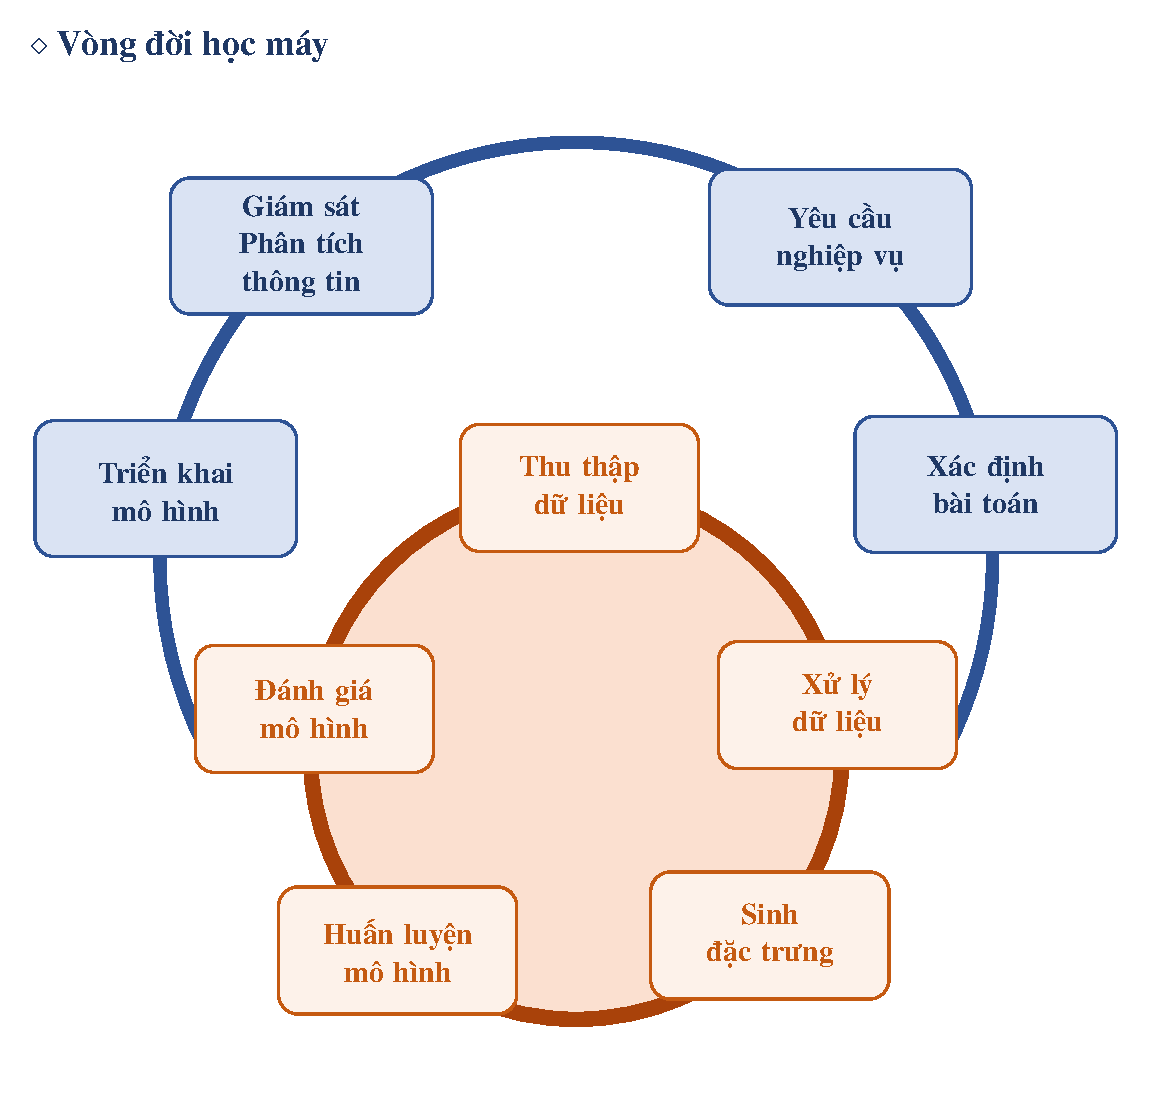
\includegraphics[width=0.60\textwidth]{sodo_ml_lifecycle_vi.pdf}
    \caption[Vòng đời học máy]{Vòng đời học máy. Nguồn: \textit{Data Version Control}~\cite{aivietnam2025dvc}.}
    \label{fig:ml_lifecycle}
\end{figure}

Quy trình của đề tài là một lần hiện thực hoá vòng đời đó.
Hình~\ref{fig:pipeline_mlops} mô tả chín bước của quy trình. Bốn bước đầu lấy, làm sạch,
chia và khảo sát dữ liệu; bước $5$ sinh rồi chọn đặc trưng; bốn bước cuối huấn luyện,
đánh giá, đưa mô hình vào sử dụng và quản lý phiên bản dữ liệu cùng mô hình.

\begin{figure}[!htbp]
    \centering
    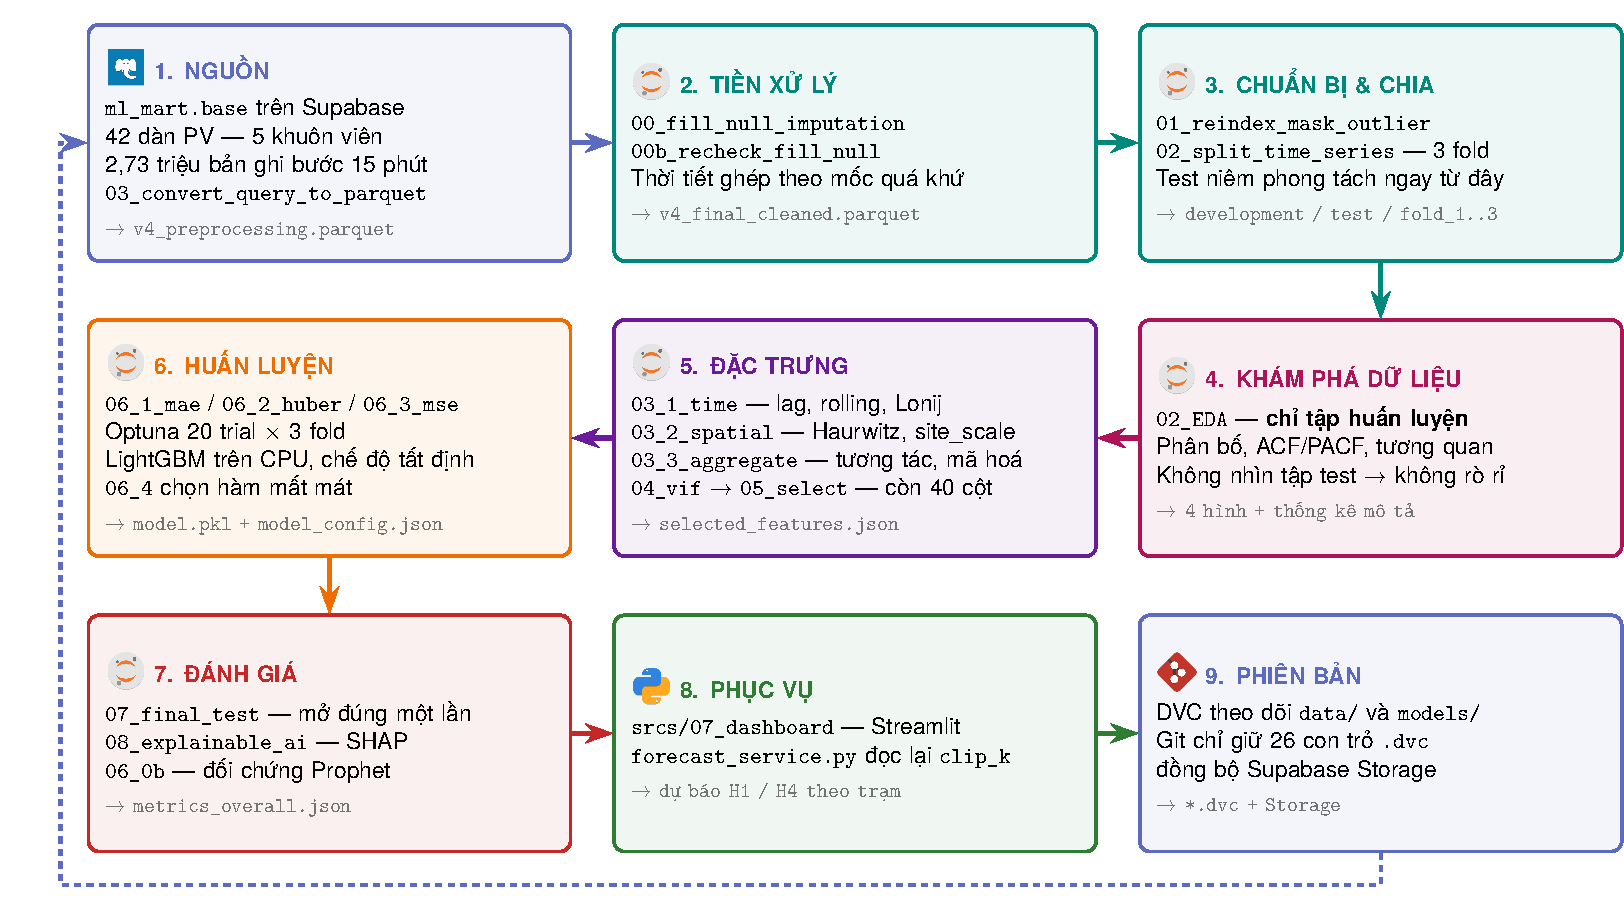
\includegraphics[width=0.96\textwidth]{pipeline_sodo_mlops.pdf}
    \caption[Chín bước của quy trình học máy]{Chín bước của quy trình học máy, xếp ba hàng ba cột và đọc theo mũi tên.
    Hàng trên chạy từ trái sang phải là bước $1$, $2$, $3$; hàng giữa chạy ngược từ phải
    sang trái là $4$, $5$, $6$; hàng dưới lại chạy từ trái sang phải là $7$, $8$, $9$.
    Dòng cuối mỗi ô ghi tệp kết quả mà bước đó sinh ra. Mũi tên nét đứt từ bước $9$ vòng
    về bước $1$ là khâu quản lý phiên bản áp lại lên tệp nguồn.}
    \label{fig:pipeline_mlops}
\end{figure}

Mỗi bước tương ứng với một notebook trong thư mục
\path{notebooks/forcasting_v4_energy/}. Toàn bộ số liệu và hình ảnh trong các phần
sau đều trích từ những tệp kết quả liệt kê ở Bảng~\ref{tab:notebook_pipeline}.

\begin{table}[htbp]
\centering

\footnotesize
% Giãn dòng toàn cục 1,35 làm bảng 13 dòng cao thêm hơn một phần tư và không nhét
% vừa phần còn lại của trang. Đưa về 1,0 trong phạm vi bảng này.
\renewcommand{\baselinestretch}{1.0}\selectfont
% Cot 3 phai du 5,4cm: ten tep dai nhat la prophet_test_summary.json, 25 ky tu chu
% don cach chiem 5,27cm. Bu lai bang cach thu cot 1 - cot do la chu tieng Viet nen
% ngat dong duoc, khong tran. Tong ba cot giu nguyen 13,4cm.
\begin{tabular}{@{}p{3.4cm} p{4.6cm} p{5.4cm}@{}}
\toprule
\textbf{Bước} & \textbf{Notebook} & \textbf{Kết quả ghi ra} \\
\midrule
Chuẩn bị lưới thời gian & \texttt{01\_reindex\_mask\_outlier} & lưới $15$ phút liên tục \\
Chia dữ liệu & \texttt{02\_split\_time\_series} & $3$ fold và tập test niêm phong \\
Khám phá dữ liệu & \texttt{02\_EDA} & thống kê mô tả, ACF/PACF, tương quan \\
Đặc trưng thời gian & \texttt{03\_1\_features\_time} & lag, rolling, chu kỳ lịch \\
Đặc trưng không gian & \texttt{03\_2\_features\_spatial} & solar geometry, \texttt{site\_scale} \\
Đặc trưng tương tác & \texttt{03\_3\_features\_aggregate} & tương tác, mã hoá phân loại \\
Chẩn đoán đa cộng tuyến & \texttt{04\_vif\_diagnostics} & bảng hệ số VIF \\
Chọn đặc trưng & \texttt{05\_select\_features} & \texttt{selected\_features.json} \\
Huấn luyện & \texttt{06\_1}, \texttt{06\_2}, \texttt{06\_3} & \texttt{model.pkl}, \texttt{model\_config.json} \\
Chọn hàm mất mát & \texttt{06\_4\_validate\_model} & bảng đối chiếu ba hàm \\
Đánh giá cuối & \texttt{07\_final\_test} & \texttt{metrics\_overall.json} \\
Giải thích mô hình & \texttt{08\_explainable\_ai} & biểu đồ SHAP \\
Mô hình đối chứng & \texttt{06\_0b\_baseline\_prophet} & \texttt{prophet\_test\_summary.json} \\
\bottomrule
\end{tabular}
\caption[Ánh xạ giữa bước trong quy trình và notebook thực hiện]{Ánh xạ giữa bước trong quy trình và notebook thực hiện.}
\label{tab:notebook_pipeline}
\end{table}

\FloatBarrier
\subsection{Năm rào chắn chống rò rỉ dữ liệu}

Rò rỉ dữ liệu là rủi ro lớn nhất của một bài toán dự báo chuỗi thời gian: chỉ cần một
đặc trưng vô tình mang thông tin của tương lai, mọi chỉ số đánh giá đều trở nên vô
nghĩa. Quy trình đặt năm rào chắn, mỗi rào chắn gắn với một bước cụ thể:

\begin{enumerate}
    \item \textbf{Nhân quả trong ghép thời tiết} (bước $2$). Mỗi bản ghi tại thời điểm
    $T$ chỉ được ghép với khối khí tượng của giờ đã kết thúc trước $T$. Điều kiện này
    được kiểm tra trên toàn bộ $2{,}73$ triệu bản ghi.

    \item \textbf{Không chồng lấn khi chia dữ liệu} (bước $3$). Dữ liệu được cắt theo
    trục thời gian, không xáo trộn ngẫu nhiên. Tập test được tách ra trước mọi bước
    khác và chỉ được mở đúng một lần ở bước $7$.

    \item \textbf{Thống kê tính riêng theo từng fold} (bước $5$). Các đại lượng tổng
    hợp như \texttt{site\_scale} hay \texttt{cs\_factor} được ước lượng riêng trong
    phần huấn luyện của từng fold, không nhìn sang phần kiểm định.

    \item \textbf{Ngưỡng suy từ dữ liệu huấn luyện} (bước $6$). Cận cắt của mục tiêu
    chuẩn hoá được tính từ phân vị của dữ liệu huấn luyện, rồi ghi vào tệp cấu hình để
    các bước sau đọc lại đúng giá trị đó thay vì tính lại trên tập khác.

    \item \textbf{Tái lập được} (bước $6$). LightGBM chạy ở chế độ tất định trên CPU;
    chạy lại với cùng hạt giống ngẫu nhiên cho ra mô hình trùng khít.
\end{enumerate}

Bốn rào chắn đầu được kiểm chứng bằng số liệu ở các phần tương ứng phía sau. Rào chắn
thứ năm được kiểm chứng bằng hai phép chạy lại độc lập, trình bày ở Mục~$7.4.5$.

\FloatBarrier
\section{Chuẩn bị dữ liệu và chia tập}

Mục này đi từ tệp đã làm sạch tới các tập sẵn sàng huấn luyện, qua sáu bước: hiện trạng dữ
liệu, dựng lại lưới thời gian, khám phá dữ liệu, cắt tập test niêm phong, chia ba fold kiểm
định, và đo nhãn chồng lấn ở ranh giới fold.

\FloatBarrier
\subsection{Hiện trạng bộ dữ liệu}

Sau khi dựng lại lưới, bộ dữ liệu có $2.784.438$ dòng của $42$ vị trí lắp đặt, trải từ
$01/01/2020$ đến $23/04/2022$ ở bước $15$ phút, trong đó $52.492$ dòng ($1{,}89\%$) là mốc
được chèn thêm cho lưới khỏi đứt quãng.

Chỉ $1.195.645$ dòng ($42{,}94\%$) là số đo thật. Phần còn lại do tầng ETL sinh ra: $1.536.301$
dòng điền khuyết ($55{,}17\%$), $42.055$ dòng gán không do sự cố thiết bị và $6.287$ dòng gán
không vì trời tối. Ngoài ra tầng ETL gắn cờ ngoại lai cho $33.280$ dòng ($1{,}20\%$), gồm
$26.318$ dòng vượt trần công suất, $5.458$ dòng do hai cơ chế thống kê cùng đồng ý, $791$ dòng
trúng nhiều luật và $713$ dòng trúng một luật vật lý khác; Mục~$7.3.2$ kiểm chứng lại các cờ này.

Bốn con số trên định hình các bước còn lại. Lưới đứt quãng phải dựng lại trước tiên, vì đặc
trưng trễ và cửa sổ trượt đếm theo số bước chứ không theo mốc đồng hồ nên một lỗ hổng làm chúng
tính sai mà không báo lỗi. Tỷ lệ đo thật thấp không sửa được bằng kỹ thuật nên xử lý bằng chính
sách: dòng không phải số đo thật, kể cả dòng mang cờ ngoại lai, nhận trọng số $0$ khi huấn luyện
và bị loại khỏi phạm vi chấm điểm, nhưng vẫn giữ trong lưới để không đứt lịch sử.

Hai điểm nữa cũng chi phối các bước sau: dữ liệu khí tượng chỉ có độ hạt một giờ nên mỗi giá trị
bức xạ lặp bốn lần và cần một bước hạ độ hạt riêng; và $42$ vị trí lắp đặt chênh nhau nhiều về
quy mô nên mục tiêu phải chuẩn hoá theo từng trạm, nếu không mô hình sẽ dồn sức phân biệt trạm
lớn với trạm nhỏ thay vì học quan hệ giữa thời tiết và sản lượng.

\FloatBarrier
\subsection{Dựng lại lưới thời gian liên tục}

Dữ liệu sản lượng thu từ công tơ không phải lúc nào cũng đủ mốc: mất điện, mất kết nối
hoặc lỗi ghi đều để lại lỗ hổng trên trục thời gian. Nếu đưa thẳng dữ liệu khuyết mốc
vào bước sinh đặc trưng, các biến trễ và biến cửa sổ trượt sẽ tính sai, \texttt{lag\_4}
lẽ ra phải lùi đúng $60$ phút thì lại lùi $75$ hay $90$ phút, tuỳ vào chỗ bị khuyết.

Notebook \tep{01_reindex_mask_outlier} dựng lại lưới $15$ phút liên tục cho từng trạm
bằng \texttt{pd.date\_range}, rồi đánh dấu những dòng vừa được chèn thêm. Thứ tự hai
việc này là điều kiện bắt buộc: dựng lưới trước, lọc sau. Nếu lọc bỏ dòng ban
đêm hay dòng ngoại lai trước khi dựng lưới, khoảng cách thời gian giữa các dòng còn lại
sẽ không đều, và mọi đặc trưng trễ sau đó đều lệch.

Các dòng bị gắn cờ ngoại lai ở tầng ETL không bị xoá khỏi lưới. Chúng được giữ nguyên
vị trí để lịch sử không bị đứt quãng, nhưng mang nhãn loại trừ nên không đóng góp vào
hàm mất mát khi huấn luyện, cũng không tham gia vào các chỉ số được báo cáo.

\textbf{Ba ràng buộc thiết kế.} Bước dựng lưới tuân thủ ba ràng buộc, cùng hướng tới một
mục tiêu: không để thông tin của tương lai, hoặc thông tin không có thật, lọt vào lưới dữ liệu.

\begin{enumerate}
    \item \textbf{Thời tiết chỉ được lấp theo chiều tiến.} Phép lấp chỉ đi từ quá khứ
    sang hiện tại, tính riêng theo từng trạm: giá trị đã quan sát ở mốc trước được đắp cho
    mốc sau. Tuyệt đối không lấp ngược chiều, vì kéo ngược là lấy giá trị của mốc sau đắp
    cho mốc trước, đúng định nghĩa của rò rỉ dữ liệu.
    \item \textbf{Metadata tĩnh thiếu thì giữ nguyên khuyết.} Các cột như
    \tep{capacity_kw}, \tep{number_of_panels}, vĩ độ và kinh độ nếu thiếu thì để nguyên
    khuyết, không lấp và không bịa giá trị.
    \item \textbf{Điền mục tiêu theo bậc thang nhân quả.} Slot mới chèn được điền theo đúng
    thứ tự: \tep{night_zero} $\rightarrow$ \tep{causal_day_persistence} (cùng giờ hôm qua)
    $\rightarrow$ \tep{causal_week_persistence} (cùng giờ tuần trước) $\rightarrow$
    \tep{causal_profile_median} $\rightarrow$ \tep{fallback_zero}. Mọi bậc đều chỉ nhìn về
    quá khứ. Riêng khoảng trống từ $24$ giờ trở lên được xếp vào \tep{machine_failure_zero}
    và đánh dấu loại khỏi huấn luyện.
\end{enumerate}

\textbf{Kết quả thực thi.} Khối dưới đây trích nguyên văn kết quả kết xuất của notebook
\tep{01_reindex_mask_outlier}:

% Khoi ket xuat notebook. Khong boc trong minipage nua: minipage la mot hop lien
% khoi, khong the ngat trang, nen khoi dai bi day nguyen sang trang sau va de lai
% khoang trong lon. De verbatim o muc doan van thi no tu ngat duoc.
\begingroup
\par\penalty-150\vspace{8pt}
\small\renewcommand{\baselinestretch}{1.0}\selectfont
\begin{verbatim}
Đã reindex lưới 15 phút cho 42 site.
Tổng số dòng sau reindex: 2784438
- Dòng gốc: 2731946
- Dòng inserted: 52492

Forward-fill thời tiết (causal only, per-site):
- Số cột thời tiết: 15
- NaN trước: 812250
- NaN sau: 1890
- Đã lấp: 810360 giá trị

Đã điền target cho 52492 slot inserted.

--- PHÂN BỐ ENERGY_SOURCE SAU CASCADE ---
energy_source
etl_imputed                1536301
measured                   1195645
machine_failure_zero         42055
night_zero                    6287
causal_day_persistence        2668
fallback_zero                  984
causal_profile_median          283
causal_week_persistence        215

--- GATE CHECK ---
- Target null: 0
- Energy_source rỗng: 0
PASS - Không còn target null hoặc energy_source rỗng.
\end{verbatim}
\par\vspace{8pt}
\endgroup
\textbf{Phân tích kết quả.} Sáu nhãn thuộc bậc thang điền, \tep{machine_failure_zero},
\tep{night_zero}, \tep{causal_day_persistence}, \tep{fallback_zero},
\tep{causal_profile_median} và \tep{causal_week_persistence}, cộng lại bằng đúng
$52.492$, tức đúng số dòng đã chèn. Không dòng nào rơi ra ngoài bậc thang, cũng không dòng
nào bị đếm hai lần. Cổng kiểm ở cuối xác nhận không còn mục tiêu khuyết và không còn
\tep{energy_source} rỗng.

\textbf{Hạn chế của bước dựng lưới.} Trong $52.492$ dòng được chèn thì $42.055$ dòng rơi vào
nhãn \tep{machine_failure_zero}, tức các khoảng trống từ $24$ giờ trở lên, được gán $0$ và
loại khỏi huấn luyện:

\begin{equation}
\frac{42.055}{52.492} = 0{,}8012 \;\longrightarrow\; \mathbf{80{,}1\%}
\end{equation}

Bốn phần năm phần chèn thêm vì vậy không mang thông tin mới; chúng chỉ giữ chỗ để
lưới thời gian không bị đứt. Phần còn lại được điền bằng các bậc suy từ lịch sử thật, gồm
$6.287 + 2.668 + 984 + 283 + 215 = 10.437$ dòng, trong đó $6.287$ dòng là \tep{night_zero}
, các mốc ban đêm vốn phải bằng $0$. Số dòng thực sự được suy từ lịch sử phát điện là
$10.437 - 6.287 = \mathbf{4.150}$ dòng.

Một hạn chế nữa: sau khi lấp theo chiều tiến vẫn còn $1.890$ ô thời tiết khuyết. Đó là các mốc
nằm ở đầu chuỗi của từng trạm, nơi chưa có quan sát quá khứ nào để kéo sang. Chỉ có thể lấp
những ô này bằng phép lấp ngược chiều, tức lấy giá trị của mốc sau đắp cho mốc trước, mà phép đó
đưa thông tin tương lai vào dữ liệu huấn luyện. Quy trình vì vậy giữ nguyên trạng thái khuyết
ở các mốc đó, đổi lấy việc bảo toàn ràng buộc nhân quả. Theo khối kết xuất ở trên, phép lấp
theo chiều tiến xử lý được $810.360$ trên $812.250$ ô khuyết ban đầu, tức
$810.360 / 812.250 = 99{,}77\%$; phần còn lại là $1.890$ ô. LightGBM nhận trực tiếp giá trị
khuyết nên phần này không cần điền.

Cách xử lý này phù hợp với kết quả của Kim, Ko và Kim~\cite{kim2019missing}. Nhóm tác
giả đánh giá tác động của dữ liệu khuyết tới bài toán dự báo sản lượng quang điện và
chỉ ra rằng cách xử lý phần khuyết ảnh hưởng trực tiếp tới sai số của mô hình dự báo,
chứ không phải là một bước tiền xử lý trung tính:

\begin{quote}\small
\textit{``Such missing values deteriorate the PV power generation prediction performance, and they need to be eliminated by filling in other values.''}
\end{quote}


Từ đó, dự án tách bạch hai việc: dựng lại mốc thời gian để cấu trúc chuỗi
không bị đứt, và đánh dấu nguồn gốc từng dòng để phần dữ liệu không đáng tin
không lọt vào chỉ số báo cáo. Phạm vi của bài báo và của dự án khác nhau ở một điểm: bài báo khảo
sát bốn phương pháp điền khuyết cho dữ liệu khí tượng và kết luận phương pháp
$k$ láng giềng gần nhất cho kết quả tốt nhất, trong khi dự án chỉ mượn kết luận tổng
quát rằng phần khuyết phải được xử lý có chủ đích.

\FloatBarrier
\subsection{Phân tích khám phá dữ liệu và các quyết định sinh đặc trưng}

Trước khi sinh đặc trưng, dữ liệu được khảo sát ở notebook \tep{02_EDA}. Phạm vi khảo sát là
chỉ tập huấn luyện, sau khi loại hai trạm $19$ và $24$: còn $1.480.000$ dòng của
$40$ trạm. Đây là điều kiện bắt buộc, các quyết định sinh đặc trưng ở Mục~$7.3$ đều rút ra
từ bước này, nên nếu khảo sát cả tập test thì tập test đã tham gia vào thiết kế mô hình,
trái với nguyên tắc niêm phong nêu ở Mục~$7.1.5$.

Ba phạm vi con được tách riêng để mọi con số phía sau đều nói rõ nó thuộc phạm vi nào:

% Khoi ket xuat notebook. Khong boc trong minipage nua: minipage la mot hop lien
% khoi, khong the ngat trang, nen khoi dai bi day nguyen sang trang sau va de lai
% khoang trong lon. De verbatim o muc doan van thi no tu ngat duoc.
\begingroup
\par\penalty-150\vspace{8pt}
\small\renewcommand{\baselinestretch}{1.0}\selectfont
\begin{verbatim}
Doc vao          : 1,550,856 dong x 12 cot | 42 tram
Sau khi bo tram [19, 24]: 1,480,000 dong | 40 tram

   toan bo               1,480,000 dong  (100.00%)
   ban ngay                742,116 dong  (50.14%)
   do that ban ngay        606,112 dong  (40.95%)
\end{verbatim}
\par\vspace{8pt}
\endgroup
\subsubsection{Phân bố đơn biến của sản lượng}

\begin{table}[htbp]
\centering

\small
\begin{tabular}{l r r r r r}
\toprule
\textbf{Phạm vi} & \textbf{Số dòng} & \textbf{Trung vị} & \textbf{Độ lệch} & \textbf{Độ nhọn} & \textbf{\% bằng $0$} \\
\midrule
Toàn bộ          & $1.480.000$ & $0{,}0000$ & $6{,}0612$ & $47{,}3723$ & $52{,}30$ \\
Ban ngày         & $742.116$   & $2{,}7325$ & $4{,}5148$ & $25{,}3908$ & $6{,}66$ \\
Đo thật ban ngày & $606.112$   & $3{,}2188$ & $4{,}4313$ & $24{,}5310$ & $0{,}00$ \\
\bottomrule
\end{tabular}
\caption[Thống kê mô tả sản lượng theo ba phạm vi]{Thống kê mô tả sản lượng theo ba phạm vi. Đọc từ ô kết quả của notebook
\tep{02_EDA.ipynb}.}
\label{tab:eda_mo_ta}
\end{table}

Phân bố lệch phải rất mạnh và nhọn: trên toàn bộ tập huấn luyện, độ lệch đạt $6{,}06$ và độ
nhọn đạt $47{,}37$, trong khi phân phối chuẩn có cả hai bằng $0$. Nguyên nhân trực tiếp là
$\mathbf{52{,}30\%}$ số quan sát bằng $0$, ban đêm và các khung giờ rìa ngày. Trung vị của
toàn bộ tập cũng bằng $0$, tức quá nửa dữ liệu không mang thông tin phát điện.

Hình~\ref{fig:eda_phan_bo} trình bày ba cách nhìn cùng một phân bố.
Lọc về ban ngày kéo độ lệch xuống $4{,}51$ và tỷ lệ giá trị $0$ xuống $6{,}66\%$; lọc thêm
điều kiện đo thật thì không còn giá trị $0$ nào. Ba dòng của Bảng~\ref{tab:eda_mo_ta} vì vậy
là căn cứ trực tiếp cho hai quyết định: chỉ tính chỉ số báo cáo trên phạm vi đo thật
ban ngày, và chuẩn hoá mục tiêu để kéo phân bố về dạng đều hơn.

\begin{figure}[htbp]
    \centering
    \includegraphics[width=\textwidth]{eda_phan_bo_don_bien.png}
    \caption[Phân bố đơn biến của sản lượng]{(Trích xuất từ Notebook \tep{02_EDA.ipynb}) \textbf{Trái:} histogram toàn bộ tập
    huấn luyện, trục tung thang loga. \textbf{Giữa:} chỉ ban ngày. \textbf{Phải:} boxplot đối
    chiếu hai phạm vi.}
    \label{fig:eda_phan_bo}
\end{figure}

\subsubsection{Mẫu hình phát điện và tác động của mây}

Hai dạng ngày cho hai dạng chuỗi khác hẳn nhau. Ngày trời quang cho đường cong trơn dạng
parabol; ngày nhiều mây cho chuỗi gãy khúc liên tục. Notebook chọn hai ngày tương phản trên
trạm phát mạnh nhất, và chỉ xét những ngày có ít nhất $40$ mốc đo thật ban ngày cùng đủ $96$
mốc trong ngày, để hình không rơi vào ngày do tầng ETL điền khuyết:

% Khoi ket xuat notebook. Khong boc trong minipage nua: minipage la mot hop lien
% khoi, khong the ngat trang, nen khoi dai bi day nguyen sang trang sau va de lai
% khoang trong lon. De verbatim o muc doan van thi no tu ngat duoc.
\begingroup
\par\penalty-150\vspace{8pt}
\small\renewcommand{\baselinestretch}{1.0}\selectfont
\begin{verbatim}
Tram 27 | 283 ngay dat dieu kien | 71 ngay nhieu nang
   Ngay troi quang: 2020-10-02 | do gap 0.0031
   Ngay nhieu may : 2020-12-23 | do gap 0.0926
\end{verbatim}
\par\vspace{8pt}
\endgroup
Hai ngày này không được chọn bằng mắt mà bằng một đại lượng đo trực tiếp trên chuỗi sản
lượng, gọi là độ gấp: trung bình trị tuyệt đối của sai phân bậc hai trong ngày, chia
cho đỉnh của chính ngày đó. Sai phân bậc hai đo mức đổi hướng giữa ba mốc liên tiếp, nên
đường càng trơn thì độ gấp càng nhỏ; phép chia cho đỉnh khiến chỉ số không phụ thuộc quy mô
trạm. Phép chọn chỉ xét trong nhóm $71$ ngày nhiều nắng, nhóm có tổng sản lượng
thuộc phần tư trên, rồi lấy ngày độ gấp nhỏ nhất làm ngày trời quang và ngày độ gấp lớn
nhất làm ngày nhiều mây. Ràng buộc nhóm là cần thiết: một ngày âm u kéo dài cũng cho đường
phẳng lì và độ gấp rất nhỏ, nếu không lọc trước thì nó sẽ bị chọn nhầm thành ngày trời quang.

Hình~\ref{fig:eda_mau_hinh} đặt hai ngày cạnh nhau trên cùng thang trục tung. Ngày
$02/10/2020$ cho một đường cong trơn, lên đều rồi hạ gần đối xứng. Ngày $23/12/2020$ đạt
đỉnh tương đương nhưng chỉ giữ được trong ít bước, phần còn lại là chuỗi răng cưa. Độ gấp của
hai ngày chênh nhau gần $30$ lần: $0{,}0926 / 0{,}0031 = 29{,}9$.

Cả hai đều thuộc nhóm ngày nhiều nắng, tức lượng bức xạ khả dụng trong ngày tương đương, nhưng
cho hai chuỗi khác hẳn. Phần chênh lệch đó là do mây, và mô hình không thể suy ra nó từ lịch
hay từ vị trí Mặt Trời. Đây là căn cứ sinh hai đặc trưng \tep{chi_so_troi_quang} và
\tep{rad_x_sinelev}: chúng cấp cho mô hình tín hiệu về mức che phủ ngay tại bước hiện
tại, thay vì bắt mô hình suy ra gián tiếp từ các mốc trễ.

\begin{figure}[htbp]
    \centering
    \includegraphics[width=\textwidth]{eda_mau_hinh_phat_dien.png}
    \caption[Sản lượng theo bước $15$ phút tại trạm $27$, hai ngày dùng chung thang trục tung]{(Trích xuất từ Notebook \tep{02_EDA.ipynb}) Sản lượng theo bước $15$ phút tại
    trạm $27$, hai ngày dùng chung thang trục tung. \textbf{Trái:} ngày trời quang
    $02/10/2020$, độ gấp $0{,}0031$. Phải: ngày nhiều mây $23/12/2020$, độ gấp
    $0{,}0926$. Trục hoành là giờ trong ngày, cắt trong khoảng $5$--$21$ giờ vì ngoài khoảng
    đó sản lượng bằng $0$. Số đo của hai ngày kiểm chứng được bằng
    \tep{srcs/05_machine_learning/kiem_chung_bao_cao_v4.py}, mục $11$.}
    \label{fig:eda_mau_hinh}
\end{figure}

% Tieu de nay chi co mot cau roi den bang, de tu nhien thi no ket thuc trang mot minh.
% Con duoi 6 dong thi day ca cum sang trang moi.
\needspace{6\baselineskip}
\subsubsection{Tự tương quan}

Bảng~\ref{tab:eda_acf} ghi tự tương quan của chuỗi sản lượng
tại các mốc trễ đáng chú ý.

\begin{table}[htbp]
\centering

\small
\begin{tabular}{l r r}
\toprule
\textbf{Mốc trễ} & \textbf{Khoảng cách} & \textbf{ACF} \\
\midrule
\texttt{lag\_1}   & $15$ phút  & $\mathbf{+0{,}9691}$ \\
\texttt{lag\_4}   & $1$ giờ    & $+0{,}9039$ \\
\texttt{lag\_96}  & $24$ giờ   & $+0{,}7138$ \\
--- & $48$ giờ & $+0{,}6506$ \\
--- & $72$ giờ & $+0{,}6274$ \\
\bottomrule
\end{tabular}
\caption[Tự tương quan của chuỗi sản lượng tại các mốc trễ đáng chú ý, trạm $27$, $42.240$ bước liên tục]{Tự tương quan của chuỗi sản lượng tại các mốc trễ đáng chú ý, trạm $27$, $42.240$
bước liên tục. Đọc từ ô kết quả của notebook \tep{02_EDA.ipynb}.}
\label{tab:eda_acf}
\end{table}

Con số $+0{,}9691$ tại mốc $15$ phút là điểm cần đọc kỹ. Ở mức tự tương quan đó, giá trị tại
$t$ gần như là bản sao của giá trị tại $t+1$, nên một mô hình được cấp \tep{lag_1} sẽ có lối
tắt hiển nhiên: lặp lại giá trị vừa đo. Mốc $1$ giờ vẫn giữ tương quan cao $+0{,}9039$ nhưng
đã đủ xa để không còn là bản sao, còn mốc $24$ giờ ở $+0{,}7138$ mang thông tin chu kỳ ngày.
Hình~\ref{fig:eda_acf} là biểu đồ đầy đủ.
Ba con số này là căn cứ định lượng cho lựa chọn trình bày ở Mục~$7.3.1$.

\begin{figure}[htbp]
    \centering
    \includegraphics[width=\textwidth]{eda_acf_pacf.png}
    \caption[Tự tương quan của chuỗi sản lượng]{(Trích xuất từ Notebook \tep{02_EDA.ipynb}) \textbf{Trái:} ACF quét $288$ bước
    $=72$ giờ. \textbf{Phải:} PACF quét $96$ bước $=24$ giờ. Vạch đỏ chấm là mốc $96$ bước.}
    \label{fig:eda_acf}
\end{figure}

\subsubsection{Tương quan giữa các biến}

Tương quan tính trên $606.112$ dòng đo thật ban ngày, xem Bảng~\ref{tab:eda_tuong_quan}.

\begin{table}[htbp]
\centering

\small
\begin{tabular}{l r r r}
\toprule
\textbf{Biến} & \textbf{Spearman ban ngày} & \textbf{Gộp cả đêm} & \textbf{Chênh} \\
\midrule
\tep{shortwave_radiation}      & $+0{,}6043$ & $+0{,}9024$ & $+0{,}2981$ \\
\tep{direct_normal_irradiance} & $+0{,}5513$ & $+0{,}8755$ & $+0{,}3243$ \\
\tep{diffuse_solar_radiation}  & $+0{,}3808$ & $+0{,}8750$ & $+0{,}4942$ \\
\tep{temperature_c}            & $+0{,}2628$ & $+0{,}4349$ & $+0{,}1721$ \\
\tep{cloud_cover_total}        & $-0{,}1591$ & $+0{,}0330$ & $+0{,}1921$ \\
\bottomrule
\end{tabular}
\caption[Tương quan với sản lượng, tính trên phạm vi đo thật ban ngày, kèm cột đối chiếu khi gộp cả ban]{Tương quan với sản lượng, tính trên phạm vi đo thật ban ngày, kèm cột đối chiếu khi
gộp cả ban đêm. Đọc từ ô kết quả của notebook \tep{02_EDA.ipynb}.}
\label{tab:eda_tuong_quan}
\end{table}

Cột chênh lệch là kết quả đáng chú ý nhất của cả bước khảo sát. Nếu gộp cả ban đêm, tương
quan của \tep{shortwave_radiation} với sản lượng vọt từ $+0{,}60$ lên $+0{,}90$, và
\tep{diffuse_solar_radiation} vọt từ $+0{,}38$ lên $+0{,}88$. Mức tăng đó không phản
ánh quan hệ vật lý: ban đêm mọi biến bức xạ và sản lượng đều bằng $0$ cùng lúc, nên hơn một
nửa số điểm nằm chồng tại gốc toạ độ và tự động đẩy hệ số tương quan lên.
Ma trận đầy đủ ở Hình~\ref{fig:eda_corr}.

Cột \tep{cloud_cover_total} cho thấy rõ nhất: ban ngày nó mang dấu âm $-0{,}1591$
, đúng ý nghĩa vật lý là mây che thì sản lượng giảm, nhưng gộp cả đêm thì đổi thành dấu
dương $+0{,}0330$, tức đảo ngược hoàn toàn ý nghĩa. Vì vậy mọi tương quan trong tài liệu này
đều tính trên phạm vi đo thật ban ngày.

\begin{figure}[htbp]
    \centering
    \includegraphics[width=0.78\textwidth]{eda_tuong_quan_spearman.png}
    \caption[Ma trận tương quan Spearman trên $606.112$ dòng đo thật ban ngày]{(Trích xuất từ Notebook \tep{02_EDA.ipynb}) Ma trận tương quan Spearman trên
    $606.112$ dòng đo thật ban ngày.}
    \label{fig:eda_corr}
\end{figure}

\textbf{Chẩn đoán đa cộng tuyến} không nằm ở bước này. Hệ số phóng đại phương sai cần toàn bộ
đặc trưng đã sinh xong, nên nó được tính ở notebook \tep{04_vif_diagnostics} và trình bày ở
Mục~$7.3.7$.

\FloatBarrier
\subsection{Chia dữ liệu theo trục thời gian}

Với bài toán dự báo, phép chia ngẫu nhiên thông thường là sai về nguyên tắc, vì cách chia đó cho
phép mô hình học từ dữ liệu của tháng sau rồi đi dự báo tháng trước. Notebook
\tep{02_split_time_series} vì vậy cắt dữ liệu theo thứ tự thời gian, không
xáo trộn.

Trước hết, $15\%$ số mốc thời gian cuối cùng được tách ra làm tập test niêm
phong và cất đi. Phần còn lại, gọi là tập Phát triển, mới được dùng để sinh đặc trưng,
chọn đặc trưng, tinh chỉnh siêu tham số (\textit{hyperparameter}) và chọn hàm mất mát. Tập test chỉ được mở đúng
một lần ở bước đánh giá cuối, sau khi mọi quyết định đã khoá.

Phép cắt thực hiện trên trục mốc thời gian, không phải trên số dòng. Toàn bộ dữ
liệu có $81.023$ mốc thời gian phân biệt; cắt $15\%$ cuối cho $12.154$ mốc thuộc tập test
và $68.869$ mốc thuộc tập Phát triển. Ranh giới rơi vào $18/12/2021$ lúc $09{:}30$:

\begin{itemize}
    \item \textbf{Tập Phát triển} --- từ $01/01/2020$ $00{:}15$ đến $18/12/2021$ $09{:}15$.
    \item \textbf{Tập test niêm phong} --- từ $18/12/2021$ $09{:}30$ đến $23/04/2022$ $23{:}45$.
\end{itemize}

Tỷ lệ $15\%$ tính trên mốc thời gian tương ứng $510.468$ dòng trên tổng $2.784.438$, tức
$18{,}33\%$ khối lượng dữ liệu. Hai tỷ lệ lệch nhau do số trạm hoạt động tăng dần
theo thời gian: đầu năm $2020$ có $30$ trạm phát sinh dữ liệu, tới cuối năm $2021$ đủ $42$
trạm, nên mỗi mốc thời gian ở giai đoạn sau mang nhiều dòng hơn giai đoạn trước.
Hình~\ref{fig:chia_du_lieu} mô tả cách chia.

Phép cắt theo mốc được chọn thay vì cắt theo số dòng vì nó cho một ranh giới thời gian duy
nhất áp dụng chung cho cả $42$ trạm. Cắt theo số dòng sẽ khiến mỗi trạm có một mốc cắt riêng
và tập test không còn là một giai đoạn liền mạch.

\begin{figure}[htbp]
    \centering
    \includegraphics[width=\textwidth]{nb02_chia_du_lieu.png}
    \caption[Cách chia dữ liệu theo trục thời gian: tập test niêm phong tách ra từ phần cuối, phần Phát]{(Trích xuất từ Notebook \tep{02_split_time_series.ipynb}) Cách chia dữ
    liệu theo trục thời gian: tập test niêm phong tách ra từ phần cuối, phần Phát triển
    còn lại chia thành ba fold theo cửa sổ mở rộng.}
    \label{fig:chia_du_lieu}
\end{figure}

\FloatBarrier
\subsection{Ba fold theo cửa sổ mở rộng}

Tập Phát triển được chia thành ba fold theo kiểu cửa sổ mở rộng
(\textit{expanding window}): phần huấn luyện của fold sau chứa trọn phần huấn luyện lẫn
phần kiểm định của fold trước. Cách này mô phỏng đúng tình huống vận hành thật, càng
về sau càng có nhiều lịch sử để học, và bảo đảm phần kiểm định luôn nằm ở tương lai
so với phần huấn luyện.

Phép chia fold cũng thực hiện trên trục mốc thời gian, mỗi fold nhận đúng $17.217$ mốc cho
phần kiểm định, còn phần huấn luyện nới rộng dần qua $17.218$, $34.435$ rồi $51.652$ mốc.

\begin{table}[htbp]
\centering

\small
\begin{tabular}{c l r c l r c}
\toprule
\textbf{Fold} & \multicolumn{3}{c}{\textbf{Phần huấn luyện}} & \multicolumn{3}{c}{\textbf{Phần kiểm định}} \\
\cmidrule(lr){2-4}\cmidrule(lr){5-7}
 & \textbf{đến} & \textbf{số dòng} & \textbf{trạm} & \textbf{đến} & \textbf{số dòng} & \textbf{trạm} \\
\midrule
$1$ & 28/06/2020 08:30 & $233.244$ & $30$ & 24/12/2020 16:45 & $606.105$ & $39$ \\
$2$ & 24/12/2020 16:45 & $839.349$ & $39$ & 22/06/2021 01:00 & $711.507$ & $42$ \\
$3$ & 22/06/2021 01:00 & $1.550.856$ & $42$ & 18/12/2021 09:15 & $723.114$ & $42$ \\
\bottomrule
\end{tabular}
\caption[Ranh giới thời gian, kích thước và số trạm của ba fold, đọc từ các tệp]{Ranh giới thời gian, kích thước và số trạm của ba fold, đọc từ các tệp
\tep{fold_*_train_selected.parquet} và \tep{fold_*_val_selected.parquet}.}
\label{tab:ba_fold}
\end{table}

Nhìn Bảng~\ref{tab:ba_fold} thấy rõ tính chất mở rộng: mốc kết thúc huấn luyện của fold
$2$ trùng đúng mốc kết thúc kiểm định của fold $1$, và tương tự giữa fold $3$ với fold
$2$. Kích thước tập huấn luyện tăng dần từ $233$ nghìn lên $1{,}55$ triệu dòng, trong
khi tập kiểm định giữ quy mô tương đương nhau, khoảng $600$--$720$ nghìn dòng.

\textbf{Vì sao chọn cửa sổ mở rộng thay vì cửa sổ trượt.} Hai cách chia đều tôn trọng
trục thời gian, khác nhau ở chỗ xử lý dữ liệu cũ. Cửa sổ mở rộng giữ lại toàn bộ quá khứ:
tập huấn luyện của fold sau chứa trọn tập huấn luyện của fold trước cộng thêm phần kiểm
định của nó, nên bề rộng lớn dần, ở đây là $233$ nghìn rồi $839$ nghìn rồi $1{,}55$ triệu
dòng. Cửa sổ trượt giữ bề rộng cố định và đẩy cả hai đầu về phía trước, tức mỗi lần tiến
một bước thì cắt bỏ một đoạn đầu tương ứng.

Ba lý do khiến cửa sổ mở rộng phù hợp với bài toán này. Thứ nhất, dữ liệu chỉ trải hơn
hai năm trong khi chu kỳ chi phối sản lượng là chu kỳ mùa dài đúng một năm; cửa sổ trượt
với bề rộng cố định sẽ khiến fold đầu tiên chỉ nhìn thấy vài tháng, không đủ trọn một
vòng mùa để học được dạng đường cong ngày của cả mùa hè lẫn mùa đông. Thứ hai, các trạm
lần lượt đi vào vận hành theo thời gian, từ $30$ trạm ở fold $1$ lên $42$ trạm ở fold $3$;
cắt bỏ đoạn đầu đồng nghĩa vứt luôn phần lịch sử sớm của những trạm vận hành trước, trong
khi đó lại chính là phần dữ liệu dài nhất của chúng. Thứ ba, quan hệ giữa bức xạ và sản
lượng của tấm quang điện là quan hệ vật lý, không đổi nhanh theo thời gian, nên dữ liệu
cũ vẫn còn giá trị mô tả.

Cửa sổ trượt sẽ là lựa chọn tốt hơn khi hệ thống có trôi khái niệm mạnh, chẳng hạn thay
tấm pin, đổi biến tần hay đổi cấu hình lắp đặt, vì khi đó dữ liệu cũ mô tả một hệ thống
khác và trở thành nhiễu. Bộ dữ liệu này không có sự kiện như vậy.

Đánh đổi phải chấp nhận là ba fold không cùng cỡ tập huấn luyện, nên sai số của từng fold
không so trực tiếp với nhau được: fold $1$ vừa ít dữ liệu vừa vướng vấn đề trạm mới nêu
ngay dưới đây. Vì vậy tài liệu chỉ dùng WAPE gộp ba fold để xếp hạng cấu hình, không đọc
riêng con số của một fold.

\textbf{Hạn chế: fold sớm có trạm chưa từng xuất hiện khi huấn luyện.} Cột số trạm trong
Bảng~\ref{tab:ba_fold} cho thấy một hệ quả trực tiếp của việc các trạm lần lượt đi vào vận
hành theo thời gian. Ở fold $1$, mô hình học trên $30$ trạm nhưng bị chấm điểm trên $39$
trạm; ở fold $2$ là $39$ trạm so với $42$. Chênh lệch đó nghĩa là một phần dữ liệu kiểm định
thuộc về những trạm mà mô hình chưa từng nhìn thấy một dòng nào lúc huấn luyện. Tới
fold $3$ thì cả $42$ trạm đều đã có mặt ở phần huấn luyện nên tình huống này không còn.

Ảnh hưởng của nó làm sai số đo trên fold $1$ và fold $2$ bi quan hơn thực tế vận
hành, vì trong vận hành thật mô hình luôn đã có lịch sử của trạm mà nó dự báo. Chiều ảnh
hưởng là an toàn, sai số bị đánh giá nặng hơn chứ không nhẹ đi, nhưng khi so sánh các
cấu hình bằng WAPE gộp ba fold thì phần đóng góp của fold $1$ vẫn mang theo thành phần sai
lệch này.

\FloatBarrier
\subsection{Thực nghiệm: đo phần chồng lấn nhãn ở ranh giới fold}

Ba fold được cắt liên tục, không chèn khoảng đệm giữa phần huấn luyện và phần kiểm
định. Hai quy tắc chống rò rỉ nêu ở Mục~$7.1.4$ chỉ ràng buộc đặc trưng đầu
vào; riêng nhãn cần một phép kiểm riêng. Nhãn của một dòng huấn luyện là sản
lượng tại $T + h$, nên với những dòng nằm sát mốc cắt, thời điểm $T + h$ có thể đã rơi
sang vùng kiểm định. Nhóm đo trực tiếp phần chồng lấn này.

\textbf{Cách tiến hành.} Với mỗi fold, phép đo đọc trực tiếp tệp huấn luyện của
chính fold đó, tức \tep{fold_i_train_selected.parquet}, rồi lấy mốc thời gian lớn nhất
$T_{\max}$ của phần huấn luyện. Một dòng có nhãn rơi sang vùng kiểm định khi và chỉ khi mốc thời gian của dòng đó lớn hơn
$T_{\max} - 15h$ phút, với $h$ là số bước của tầm dự báo. Đếm số dòng thoả điều kiện đó
cho cả hai tầm H1 và H4. Phép đo chạy trên chính các tệp fold mà bước huấn luyện đọc
vào, không dùng dữ liệu trung gian nào khác.

\begin{table}[htbp]
\centering

\small
\begin{tabular}{c r r r r}
\toprule
\textbf{Fold} & \textbf{Cỡ tập huấn luyện} & \textbf{Chồng lấn H1} & \textbf{Chồng lấn H4} & \textbf{Tỷ lệ H4} \\
\midrule
$1$ & $233.244$ & $30$ & $120$ & $0{,}0514\%$ \\
$2$ & $839.349$ & $39$ & $156$ & $0{,}0186\%$ \\
$3$ & $1.550.856$ & $42$ & $168$ & $0{,}0108\%$ \\
\bottomrule
\end{tabular}
\caption[Số dòng huấn luyện có nhãn rơi sang vùng kiểm định, tính trên từng fold và từng tầm dự báo]{Số dòng huấn luyện có nhãn rơi sang vùng kiểm định, tính trên từng fold và
từng tầm dự báo. Đọc từ ô kết quả của notebook
\tep{05b_thuc_nghiem_tham_so_hardcode.ipynb}, Thí nghiệm $9$.}
\label{tab:chong_lan}
\end{table}

Trường hợp xấu nhất là fold $1$ ở tầm H4: $120$ dòng trên $233.244$, tức
$\mathbf{0{,}0514\%}$. Tỷ lệ nhỏ như vậy là hệ quả cấu trúc của phép cắt, chỉ những dòng
nằm trong $h$ bước cuối cùng của tập huấn luyện mới có nhãn vượt sang vùng kiểm định, mà
$h$ nhiều nhất là bốn bước.

Bảng~\ref{tab:chong_lan} tự kiểm chứng được. Ở tầm H1 chỉ một bước cuối bị chồng
lấn, nên số dòng phải bằng số trạm còn hoạt động tại bước đó: cột chồng lấn H1 cho $30$,
$39$ và $42$, trùng khít cột số trạm ở Bảng~\ref{tab:ba_fold}. Cột H4 gấp đúng bốn lần các
giá trị đó.

Với mức chồng lấn dưới một phần nghìn ở cả ba fold, phép cắt liên tục được giữ nguyên,
không chèn khoảng đệm.

\FloatBarrier
\section{Sinh đặc trưng}

Mục này đi qua ba họ đặc trưng --- thời gian và lịch sử sản lượng, solar geometry và chuẩn
hoá theo trạm, tương tác khí tượng và mã hoá phân loại --- rồi định nghĩa đặc trưng dẫn xuất,
khử độ trễ cài sẵn, chuẩn hoá mục tiêu, kiểm chứng tham số cố định, và chốt danh sách cuối.

\FloatBarrier
\subsection{Đặc trưng thời gian, trễ và cửa sổ trượt}

Notebook \tep{03_1_features_time} sinh ba nhóm đặc trưng, tóm tắt ở
Bảng~\ref{tab:dac_trung_thoi_gian}.

\begin{table}[htbp]
\centering

\small
\begin{tabular}{@{}L{2.8cm} L{6.6cm} L{4.7cm}@{}}
\toprule
\textbf{Nhóm} & \textbf{Cột sinh ra} & \textbf{Tham số} \\
\midrule
Lịch và chu kỳ &
\texttt{minute\_of\_day}, \texttt{month}, \texttt{day\_of\_week}, \texttt{is\_weekend},
\texttt{season}, \texttt{season\_code}, \texttt{hour\_sin}, \texttt{hour\_cos},
\texttt{doy\_sin}, \texttt{doy\_cos} &
chu kỳ ngày $1440$ phút; chu kỳ năm $365{,}25$ ngày \\
\addlinespace
Trễ &
\texttt{lag\_4}, \texttt{lag\_96} &
\texttt{LAGS} $= (4,\ 96)$, tức $T - 60$ phút và $T - 24$ giờ \\
\addlinespace
Cửa sổ trượt &
\texttt{rolling\_mean}, \texttt{rolling\_std}, \texttt{rolling\_min},
\texttt{rolling\_max} cho mỗi cửa sổ &
\texttt{ROLLING\_WINDOWS} $= (4,\ 96)$, bốn thống kê mỗi cửa sổ \\
\bottomrule
\end{tabular}
\caption[Ba nhóm đặc trưng sinh tại notebook \tep{03_1_features_time.ipynb}]{Ba nhóm đặc trưng sinh tại notebook \tep{03_1_features_time.ipynb}. Cột cuối ghi
tham số thực tế khai báo trong notebook.}
\label{tab:dac_trung_thoi_gian}
\end{table}

Hai nhóm sau tạo ra $2$ cột trễ cộng $8$ cột cửa sổ trượt, bằng $10$ cột suy từ chuỗi mục
tiêu, đúng con số notebook in ra khi khai báo hàm sinh đặc trưng.

\textbf{Mã hoá lịch bằng sin và cos.} Nếu để giờ trong ngày ở dạng số nguyên, mốc $23{:}45$
và mốc $00{:}00$ cách nhau đúng một bước $15$ phút trên thực tế nhưng cách nhau $23$ đơn vị
trên thang số. Cây quyết định chia theo ngưỡng sẽ coi hai mốc liền kề đó là hai vùng xa
nhau. Cặp $(\sin, \cos)$ đưa trục thời gian về một vòng tròn khép kín, nên khoảng cách giữa
hai mốc kề nhau qua nửa đêm trở lại đúng bằng khoảng cách thật. Cùng lý do, ngày trong năm
được mã hoá bằng \texttt{doy\_sin} và \texttt{doy\_cos} theo chu kỳ $365{,}25$ ngày.

\subsubsection{Thực nghiệm: chọn mốc trễ}

\textbf{Khái niệm nền.} \textit{Persistence} là mô hình dự báo cơ sở: lấy giá trị quan sát
tại $t$ làm dự báo cho $t+h$. Dev và cộng sự~\cite{dev2018tes} định nghĩa nó là phương pháp
\textit{giả định điều kiện tại thời điểm dự báo không thay đổi so với thời điểm quan sát},
và ghi nhận rằng cách này \textit{chạy tốt} ở các tầm dự báo ngắn, khi điều kiện thời tiết
biến thiên chậm:

\begin{quote}\small
\textit{``The persistence forecasting method assumes that the conditions for the forecast do not change (especially for shorter lead times). This method works well in conditions when weather maps change very slowly with time.''}
\end{quote}


Từ định nghĩa trên suy ra một hệ quả đại số mà bài báo không nêu: nếu $\hat{y}(t+h) = y(t)$
thì đường dự báo chính là đường đo thật dịch phải $h$ bước, tức lệch pha đúng bằng
tầm dự báo. Mặt khác, vì chuỗi biến thiên chậm ở tầm ngắn, đúng điều kiện mà bài báo nói
\textit{persistence} chạy tốt, nên hiệu giữa $y(t)$ và $y(t+h)$ nhỏ, và một chỉ số sai số
tính theo từng điểm vẫn cho con số đẹp.

Tầm H1 của dự án đúng bằng $15$ phút, nằm trọn trong vùng đó. Một mô hình lặp lại giá trị vừa
đo sẽ cho chỉ số sai số tốt nhưng đường dự báo trễ một nhịp, con số đẹp
ở đây không chứng minh năng lực dự báo.

\textbf{Giả thuyết.} Mốc trễ càng gần thời điểm dự báo thì tín hiệu càng mạnh, nhưng cũng
càng dễ kéo mô hình về đúng dạng vừa nêu. Thực nghiệm này xác định mốc trễ nào được đưa vào.

\textbf{Cách tiến hành.} Ba cấu hình được đối chiếu trên cùng dữ liệu và cùng quy trình tinh
chỉnh: cấu hình nền chỉ có \texttt{lag\_96} ($T - 24$ giờ), cấu hình thêm \texttt{lag\_1}
($T - 15$ phút), và cấu hình thêm \texttt{lag\_4} ($T - 60$ phút). Mỗi cấu hình được chấm
bằng WAPE và một phép đo lệch pha riêng: độ trễ trung bình giữa đường dự báo và
đường đo thật trên từng trạm, kèm số trạm vượt ngưỡng cho phép. Ba mốc đã thử ghi ở
Bảng~\ref{tab:chon_lag}.

\begin{table}[htbp]
\centering

\small
\begin{tabular}{@{}L{3.4cm} L{3.6cm} L{7.0cm}@{}}
\toprule
\textbf{Mốc trễ} & \textbf{Quyết định} & \textbf{Căn cứ ghi trong notebook} \\
\midrule
\texttt{lag\_96} ($T-24$ giờ) & \textbf{giữ} &
Chu kỳ ngày; xa thời điểm dự báo nên không tạo lệch pha \\
\addlinespace
\texttt{lag\_1} ($T-15$ phút) & \textbf{loại} &
Gây lệch pha trên gần như toàn bộ đội hình; sai số theo từng điểm giảm nhưng là hệ quả của
việc lặp lại giá trị vừa đo \\
\addlinespace
\texttt{lag\_4} ($T-60$ phút) & \textbf{giữ} &
Đủ xa để không lặp lại được giá trị vừa đo, vẫn đủ gần để mang thông tin quán tính; qua được
cổng lệch pha ở Mục~$7.3.1$ \\
\bottomrule
\end{tabular}
\caption[Ba mốc trễ đã được thử và quyết định tương ứng, ghi tại ô khai báo \texttt{LAGS} của notebook]{Ba mốc trễ đã được thử và quyết định tương ứng, ghi tại ô khai báo \texttt{LAGS} của
notebook \tep{03_1_features_time.ipynb}.}
\label{tab:chon_lag}
\end{table}

\textbf{Đọc kết quả.} Quyết định phân biệt \texttt{lag\_1} với \texttt{lag\_4} không dựa vào
sai số mà dựa vào lệch pha. Nếu chỉ nhìn WAPE thì \texttt{lag\_1} sẽ được chọn, vì
nó cho con số thấp nhất, đúng như hệ quả đại số nêu ở đầu mục. Dự án chốt \texttt{LAGS}
$= (4,\ 96)$ và loại \texttt{lag\_1}.

Cần nêu rõ giới hạn của bằng chứng này: notebook ghi lại quyết định và căn
cứ định tính, không lưu một phép đối chứng có kiểm soát giữa ba cấu hình trên cùng một lần
chạy. Bằng chứng định lượng cho cấu hình được chọn nằm ở cổng lệch pha trình bày ngay sau
đây.

\subsubsection{Cổng lệch pha đặt trước bước tinh chỉnh}

Phép đo lệch pha được đặt thành một cổng chặn ở đầu notebook huấn luyện: chỉ khi cổng đạt
thì quy trình mới được phép chạy Optuna và huấn luyện thật.

Độ trễ suy từ quan hệ giữa sai số và độ dốc của đường đo thật. Nếu đường dự báo bị dịch
$c$ bước thì sai số xấp xỉ $-c$ nhân với độ dốc, nên hệ số hồi quy của sai số theo độ dốc
chính là $c$:

\begin{equation}
\text{độ trễ (phút)} \;=\; -\,\frac{\sum_t d_t \, e_t}{\sum_t d_t^{2}} \times 15,
\qquad
d_t = \frac{y_{t+1} - y_{t-1}}{2}, \quad e_t = \hat{y}_t - y_t .
\end{equation}

Cách này tách sai số biên độ khỏi sai số thời điểm: dự báo cao hơn hay thấp hơn thực tế
đều không làm đổi con số, chỉ việc đến sớm hay đến muộn mới làm đổi.

Cổng chạy trên một mô hình nháp dùng cùng thuật toán LightGBM, cùng hàm mất mát MAE và
cùng $54$ đặc trưng với mô hình cuối, nhưng chỉ học $300.000$ dòng lấy ngẫu nhiên với
$200$ cây, tốc độ học $0{,}08$ và \texttt{num\_leaves} $=63$ đặt cố định, chạy xong trong
$9{,}3$ giây. Giữ nguyên bộ đặc trưng là điều kiện then chốt, vì cổng kiểm đúng thứ nó
cần kiểm: bộ đặc trưng có đẩy mô hình vào hành vi bám trụ hay không. Nếu \texttt{lag\_1}
có mặt thì mô hình nháp cũng sao chép giá trị gần nhất y như mô hình cuối.

Ngưỡng là $\pm 5$ phút và không trạm nào được vượt. Đo trên $288.735$ điểm ban ngày, độ
trễ là $+2{,}46$ phút, trung vị theo trạm $+2{,}79$ phút, dao động từ $+1{,}64$ đến
$+3{,}71$, và $0/40$ trạm vượt ngưỡng, nên cổng đạt. Cổng này đặt trước bước tinh chỉnh
nên chỉ kiểm bộ đặc trưng; sau khi Optuna chọn xong siêu tham số (\textit{hyperparameter}), notebook chạy tiếp một
phép quét độ trễ thứ hai trên toàn bộ tập kiểm định, trình bày ở phần đánh giá.

\subsubsection{Rào chắn chống rò rỉ và ngữ cảnh lùi}

Bước sinh đặc trưng đặt hai rào chắn. Một, mọi đặc trưng suy từ mục tiêu đều được dịch:
các cột cửa sổ trượt tính trên chuỗi mục tiêu đã dịch một bước, nên giá trị tại $T$ không
bao giờ chứa sản lượng đo tại chính $T$. Hai, một mặt nạ lịch sử liên tục kiểm tra toàn
bộ số bước của cửa sổ liền trước đều cách nhau đúng $15$ phút; cửa sổ vắt qua chỗ đứt gãy
thì bị gán khuyết thay vì tính bừa trên hai đoạn không liền nhau.

Ngữ cảnh lùi giải quyết vế còn lại: mỗi tập được nối thêm lịch sử của tập liền trước
trước khi tính đặc trưng, rồi chỉ xuất phần dòng thuộc chính tập đó. Tập test dùng toàn
bộ tập Phát triển làm ngữ cảnh, tập kiểm định dùng tập huấn luyện, và phần kiểm định của
mỗi fold dùng phần huấn luyện của chính fold đó. Nhờ vậy dòng đầu tiên của mỗi tập vẫn có
đủ lịch sử, mà mỗi fold vẫn là một thí nghiệm khép kín.

Kết xuất của notebook \tep{03_1_features_time} xác nhận $10$ cột suy từ mục tiêu ($2$ cột
trễ và $8$ cột cửa sổ trượt) và lưới thời gian liên tục $100\%$, không còn điểm đứt gãy
nào. Ô khuyết chỉ còn $21.000$ dòng ở tập huấn luyện, nằm tại các dòng đầu chuỗi chưa đủ
$96$ bước lịch sử để tính cửa sổ dài; tập kiểm định và tập test không còn ô khuyết nào
nhờ ngữ cảnh lùi.

\FloatBarrier
\subsection{Solar geometry, bức xạ trời quang và chuẩn hoá theo trạm}

Notebook \tep{03_2_features_spatial} sinh nhóm đặc trưng suy từ vị trí Mặt Trời, còn
\tep{03_3_features_aggregate} sinh nhóm tương tác khí tượng và mã hoá biến phân loại. Cả hai
nhóm đều là hàm xác định của thời gian và vị trí hoặc là tổ hợp của các biến đã có,
nên không mang rủi ro rò rỉ.

\subsubsection{Vị trí Mặt Trời theo thuật toán NOAA}

Góc cao $h$ và góc phương vị được tính theo thuật toán vị trí Mặt Trời chuẩn của NOAA,
chuỗi Fourier cho độ xích vĩ, phương trình thời gian và góc giờ. Bản tham chiếu là NOAA
Solar Calculator do Global Monitoring Laboratory thuộc Cơ quan Khí quyển và Đại dương
Quốc gia Hoa Kỳ công bố; hàm \tep{tinh_goc_mat_troi} của dự án cài đặt lại đúng chuỗi
công thức đó, chỉ khác ở chỗ nhận cả một vector mốc thời gian thay vì từng mốc lẻ.

Ba chi tiết cài đặt đáng nêu, tóm tắt ở Bảng~\ref{tab:chi_tiet_solar}.

\begin{table}[htbp]
\centering

\small
\begin{tabular}{@{}L{2.8cm} L{5.4cm} L{6.4cm}@{}}
\toprule
\textbf{Chi tiết} & \textbf{Trong mã nguồn} & \textbf{Lý do} \\
\midrule
Quy đổi về giờ UTC &
\texttt{utc = ts - tz\_gio}, với \texttt{tz\_gio} bằng $11$ cho tháng $10$--$3$ và $10$ cho
tháng $4$--$9$ &
Mốc trong dữ liệu là \textbf{giờ địa phương của Úc}, còn công thức thiên văn cần giờ UTC.
Úc áp dụng giờ mùa hè nên độ lệch đổi theo mùa \\
\addlinespace
Góc phương vị &
\texttt{np.arctan2(...)} thay cho $\arccos$ &
$\arccos$ chỉ trả về miền $[0^\circ;\ 180^\circ]$ nên không phân biệt được buổi sáng với
buổi chiều; $\operatorname{atan2}$ liên tục trên trọn vòng $360^\circ$ \\
\addlinespace
Dạng vòng của góc &
\texttt{azimuth\_sin}, \texttt{azimuth\_cos} &
Góc đo bằng độ gián đoạn ở mốc $0^\circ$ và $360^\circ$: $359^\circ$ và $1^\circ$ kề nhau
thực tế nhưng cách xa trên thang số \\
\bottomrule
\end{tabular}
\caption[Ba chi tiết cài đặt của bước solar geometry]{Ba chi tiết cài đặt của bước solar geometry.}
\label{tab:chi_tiet_solar}
\end{table}

Cách cắt mùa theo nguyên tháng là một xấp xỉ: giờ mùa hè ở Úc bắt đầu Chủ nhật đầu
tiên của tháng $10$ và kết thúc Chủ nhật đầu tiên của tháng $4$, nên vài ngày đầu hai tháng
đó nhận độ lệch chênh một giờ, khoảng $12$ ngày mỗi năm.

\subsubsection{Bức xạ trời quang theo mô hình Haurwitz}

\textbf{GHI} (\textit{Global Horizontal Irradiance}) là tổng bức xạ Mặt Trời chiếu
xuống một mặt phẳng nằm ngang, đơn vị W/m\textsuperscript{2}. Nó gồm hai thành phần cộng
lại: phần trực xạ đi thẳng từ đĩa Mặt Trời và phần khuếch tán do bầu khí quyển và mây tán
xạ. Trong dữ liệu của dự án, hai đại lượng này nằm ở hai cột khác nhau và không được
lẫn:

\begin{itemize}
    \item \tep{shortwave_radiation}, GHI đo được thực tế, do Open-Meteo cung cấp.
    \item \tep{ghi_cs}, $GHI_{cs}$, giá trị lý thuyết khi trời hoàn toàn quang, do nhóm
    tự tính bằng mô hình Haurwitz từ góc cao Mặt Trời.
\end{itemize}

Vì $GHI_{cs}$ ứng với điều kiện không mây, nó là mức trần mà bức xạ đo được chỉ có thể tiệm
cận chứ không nên vượt qua.

Từ góc cao suy ra bức xạ ngang trời quang:

\begin{equation}
GHI_{cs} = 1098 \times \sin(h) \times \exp\!\left(-\frac{0{,}059}{\sin(h)}\right)
\quad (\mathrm{W/m^2})
\end{equation}

Cặp hằng số $1098$ và $0{,}059$ lấy đúng bản cài đặt Haurwitz của thư viện \texttt{pvlib},
vốn dẫn về hai bài gốc của Haurwitz~\cite{haurwitz1945}. Phần tóm tắt của bài báo
nguồn phát biểu dạng công thức như sau:

\begin{quote}\small
\textit{``These relations are of the form $T = (a/m)e^{-bm}$ where $m$ = air mass (i.e. secant of zenith distance of the sun), $e$ = base of natural logarithms, $a$ and $b$ are constants which depend on the cloudiness and cloud density.''}
\end{quote}


Mô hình trời quang thuần thiên văn ước lượng thiếu so với bức xạ đo tại các trạm, nên
$GHI_{cs}$ được nhân thêm hệ số hiệu chỉnh riêng từng trạm, đặt tên \tep{cs_factor}. Hệ số
này tính riêng trên phần huấn luyện của từng fold, xem Bảng~\ref{tab:cs_factor}.

\begin{table}[htbp]
\centering

\small
\begin{tabular}{l r r r}
\toprule
\textbf{Phạm vi tính} & \textbf{Trung vị} & \textbf{Nhỏ nhất} & \textbf{Lớn nhất} \\
\midrule
Phần huấn luyện fold $1$ & $1{,}460$ & $1{,}105$ & $1{,}827$ \\
Phần huấn luyện fold $2$ & $1{,}538$ & $1{,}520$ & $1{,}819$ \\
Phần huấn luyện fold $3$ & $1{,}557$ & $1{,}541$ & $1{,}809$ \\
\bottomrule
\end{tabular}
\caption[Hệ số hiệu chỉnh trời quang \tep{cs_factor} theo từng fold]{Hệ số hiệu chỉnh trời quang \tep{cs_factor} theo từng fold. Đọc từ ô kết quả của
notebook \tep{03_2_features_spatial.ipynb}.}
\label{tab:cs_factor}
\end{table}

Giá trị đổi rõ giữa các fold, trung vị từ $1{,}460$ lên $1{,}557$, nên việc dùng chung
một bộ thống kê cho cả ba fold sẽ đưa thông tin của giai đoạn sau vào fold sớm. Notebook ghi
thẳng nguyên tắc này ở ô kết quả: \textit{mỗi fold dùng thống kê quy mô tính riêng từ tập
train của chính fold đó}.

\subsubsection{Thực nghiệm: hạ độ hạt bức xạ từ một giờ về mười lăm phút}

\textbf{Vấn đề.} Dữ liệu khí tượng có tần suất một giờ, còn lưới sản lượng có tần suất $15$
phút, nên mỗi giá trị bức xạ lặp lại bốn lần liên tiếp: trong một giờ, đặc trưng bức xạ không
phân biệt được mốc $12{:}00$ với mốc $12{:}15$.

\textbf{Nguyên lý.} Bailey và cộng sự~\cite{bailey2024} mô tả thuật toán của Graham và
Hollands ($1990$): tách chỉ số trời quang theo giờ $k_t$ thành mô hình cộng
$k_t = k_{tm} + \alpha$ gồm thành phần xu thế và thành phần nhiễu. Điểm cốt lõi là hạ độ hạt của chỉ số trời quang chứ không phải bức xạ, vì bức xạ mang cả biến thiên nhật
triều, còn chỉ số trời quang thì không.

Dự án giữ đúng thành phần xu thế $k_{tm}$, giữ chỉ số trời quang không đổi trong mỗi khối
giờ rồi nhân lại với $GHI_{cs}$ tính ở từng mốc $15$ phút, và bỏ thành phần nhiễu $\alpha$,
vì $\alpha$ dùng để sinh chuỗi tổng hợp, còn ở đây bức xạ là đặc trưng đầu vào cho mô hình
dự báo.

\textbf{Kết quả đo.} Thước đo là tỷ lệ bước có giá trị bức xạ thay đổi so với bước liền
trước, tính riêng trên các dòng ban ngày. Khối kết quả của notebook:

% Khoi ket xuat notebook. Khong boc trong minipage nua: minipage la mot hop lien
% khoi, khong the ngat trang, nen khoi dai bi day nguyen sang trang sau va de lai
% khoang trong lon. De verbatim o muc doan van thi no tu ngat duoc.
\begingroup
\par\penalty-150\vspace{8pt}
% \footnotesize thay vi \small: dong tieu de cua khoi nay dai hon kho chu 44pt nen o
% co \small no tran ra ngoai le phai. Ha co chu la cach duy nhat giu duoc NGUYEN VAN
% tung ky tu output cua notebook - ngat dong hay bo bot chu deu lam sai ban trich.
\footnotesize\renewcommand{\baselinestretch}{1.0}\selectfont
\begin{verbatim}
--- TY LE BUOC CO GIA TRI BUC XA THAY DOI, TOAN TAP TRAIN (CHI BAN NGAY) ---
   So dong ban ngay: 751,408 / 1,550,856 (48.5%)
   Truoc downscale :  26.7%
   Sau  downscale  :  76.7%
Muc tieu la tren 90 phan tram.
   [CANH BAO] Chua dat 90 phan tram, kiem lai buoc downscale.
\end{verbatim}
\par\vspace{8pt}
\endgroup
Tỷ lệ tăng gần ba lần, từ $26{,}7\%$ lên $76{,}7\%$. Hình~\ref{fig:downscale} cho thấy hiệu
quả trên một cửa sổ sáu giờ.

\begin{figure}[htbp]
    \centering
    \includegraphics[width=\textwidth]{nb032_downscale_truoc_sau.png}
    \caption[Bức xạ tại trạm $1$, ngày $19/12/2020$, từ $11$ giờ đến $17$ giờ]{(Trích xuất từ Notebook \tep{03_2_features_spatial.ipynb}) Bức xạ tại trạm $1$,
    ngày $19/12/2020$, từ $11$ giờ đến $17$ giờ. \textbf{Trên:} dữ liệu gốc theo giờ, mỗi
    giá trị lặp bốn lần nên đường đi thành bậc thang. Dưới: sau khi hạ độ hạt,
    đường biến thiên theo từng bước $15$ phút.}
    \label{fig:downscale}
\end{figure}

\subsubsection{Chuẩn hoá quy mô theo trạm}

Bốn mươi hai vị trí lắp đặt điện mặt trời có quy mô rất khác nhau, nên quy mô được ước lượng từ chính dữ
liệu và chỉ từ phần huấn luyện: \tep{site_scale} là phân vị $99$ của sản lượng ban
ngày, \tep{tran_cong_suat} là phân vị $99{,}9$. Bảng~\ref{tab:quy_mo} trích tám trạm đầu
trong bảng notebook in ra.

\begin{table}[htbp]
\centering

\small
\begin{tabular}{r r r r}
\toprule
\textbf{Trạm} & \tep{site_scale} & \tep{tran_cong_suat} & \tep{cs_factor} \\
\midrule
$27$ & $97{,}19$ & $99{,}00$ & $1{,}55$ \\
$11$ & $92{,}05$ & $92{,}72$ & $1{,}74$ \\
$25$ & $79{,}73$ & $82{,}42$ & $1{,}55$ \\
$19$ & $41{,}73$ & $42{,}80$ & $1{,}55$ \\
$18$ & $35{,}04$ & $36{,}21$ & $1{,}55$ \\
$6$  & $27{,}53$ & $28{,}51$ & $1{,}74$ \\
$8$  & $26{,}50$ & $26{,}89$ & $1{,}74$ \\
$1$  & $21{,}50$ & $22{,}73$ & $1{,}70$ \\
\bottomrule
\end{tabular}
\caption[Quy mô trạm tính trên tập huấn luyện, tám trạm lớn nhất]{Quy mô trạm tính trên tập huấn luyện, tám trạm lớn nhất. Đọc từ ô kết quả của
notebook \tep{03_2_features_spatial.ipynb}.}
\label{tab:quy_mo}
\end{table}

Một mô hình học thẳng trên sản lượng thô sẽ dành phần lớn sức mô tả để phân biệt trạm lớn với trạm nhỏ, thay vì học quan hệ
giữa thời tiết và sản lượng, đó là lý do mục tiêu được chuẩn hoá trước khi huấn luyện.

\subsubsection{Tương tác khí tượng và mã hoá biến phân loại}

Notebook \tep{03_3_features_aggregate} sinh năm đặc trưng tương tác, xem
Bảng~\ref{tab:tuong_tac}.

\begin{table}[htbp]
\centering

\small
% Cot 1 phai du 5,0cm: ten dai nhat la cloud_low_x_shortwave, 21 ky tu chu don cach o
% co \small chiem 4,85cm. De 4,4cm thi no tran khoi cot va dinh lien vao chu cua cot
% "Dinh nghia" ben canh, mat han khoang cach giua hai cot.
\begin{tabular}{@{}L{5.0cm} L{4.6cm} r r@{}}
\toprule
\textbf{Đặc trưng} & \textbf{Định nghĩa} & \textbf{Khuyết} & \textbf{Pearson} \\
\midrule
\texttt{temp\_x\_shortwave} & nhiệt độ $\times$ bức xạ ngang & $0{,}01\%$ & $0{,}3487$ \\
\texttt{diffuse\_ratio} & bức xạ khuếch tán $/$ bức xạ ngang & $47{,}43\%$ & $-0{,}2350$ \\
\texttt{dni\_ratio} & bức xạ trực xạ $/$ bức xạ ngang & $47{,}43\%$ & $0{,}2350$ \\
\texttt{cloud\_x\_shortwave} & mây toàn phần $\times$ bức xạ ngang & $0{,}01\%$ & $0{,}1921$ \\
\texttt{cloud\_low\_x\_shortwave} & mây tầng thấp $\times$ bức xạ ngang & $0{,}01\%$ & $0{,}1650$ \\
\bottomrule
\end{tabular}
\caption[Năm đặc trưng tương tác, tỷ lệ khuyết trên tập huấn luyện và tương quan Pearson với mục tiêu]{Năm đặc trưng tương tác, tỷ lệ khuyết trên tập huấn luyện và tương quan Pearson với
mục tiêu tính trên $763.740$ dòng ban ngày. Đọc từ ô kết quả của notebook
\tep{03_3_features_aggregate.ipynb}.}
\label{tab:tuong_tac}
\end{table}

Tỷ lệ khuyết $47{,}43\%$ ($735.612$ dòng) của hai đặc trưng dạng thương đến từ mẫu số: ban
đêm bức xạ ngang bằng $0$ nên phép chia không xác định. Giá trị khuyết được giữ nguyên thay
vì điền $0$, để mô hình cây học nhánh riêng cho dữ liệu khuyết. Số giá trị vô cực trên cả
năm cột bằng $0$.

\textbf{Mã hoá biến phân loại.} Bảng mã được khớp chỉ trên phía huấn luyện rồi áp
cho phía kiểm định; notebook khớp được $8$ bảng mã, và số ô gặp hạng mục lạ trên tập kiểm
định bằng $0$.

\textbf{Kiểm chứng cuối bước sinh đặc trưng.} Notebook in ra ba phép kiểm:

% Khoi ket xuat notebook. Khong boc trong minipage nua: minipage la mot hop lien
% khoi, khong the ngat trang, nen khoi dai bi day nguyen sang trang sau va de lai
% khoang trong lon. De verbatim o muc doan van thi no tu ngat duoc.
\begingroup
\par\penalty-150\vspace{8pt}
\small\renewcommand{\baselinestretch}{1.0}\selectfont
\begin{verbatim}
--- KIEM TRA 1: dac trung target deu duoc shift ---
Cot lag con lai sau khi khu tre pha: ['lag_4', 'lag_96']
lag_96(t) == target(t-96) tren mau: DAT
--- KIEM TRA 2: ty le dong co lich su day du ---
- train       : 99.74% dong co du lich su lien tuc
- val         : 100.00% dong co du lich su lien tuc
--- KIEM TRA 3: hang muc la (unseen category) ---
Tong so o gap hang muc la trong val: 0
\end{verbatim}
\par\vspace{8pt}
\endgroup
Sau ba notebook sinh đặc trưng, tập huấn luyện đi từ $50$ cột lên $114$ cột, trong đó $46$
cột là đặc trưng ứng viên; các fold mang $115$ cột do có thêm cột đánh dấu fold.

\FloatBarrier
\subsection{Định nghĩa các đặc trưng dẫn xuất}

Một số cột xuất hiện trong bảng chẩn đoán và bảng chấm điểm ở Mục~$7.3.7$ là đại lượng dẫn xuất,
không đọc thẳng từ dữ liệu nguồn. Bảng~\ref{tab:dinh_nghia_dan_xuat} ghi công thức của chúng.

\begin{table}[htbp]
\centering

\small
% Cot 2 phai du 7,0cm: o dai nhat la cong thuc clip(shortwave_radiation/ghi_cs, 0, 1,5)
% dat trong \dfrac, khong ngat dong duoc. Bu lai bang cach thu cot 1 (ten cot ngan
% nhat can 3,93cm) va cot 3 (chu tieng Viet, ngat dong duoc). Tong giu nguyen 15,1cm.
\begin{tabular}{@{}L{4.0cm} L{7.0cm} L{4.1cm}@{}}
\toprule
\textbf{Đặc trưng} & \textbf{Công thức} & \textbf{Ý nghĩa} \\
\midrule
\tep{ky_vong} &
$\texttt{site\_scale} \times \max(\sin h,\ 0)$ &
Mức sản lượng kỳ vọng của trạm tại góc cao hiện tại, nếu trời hoàn toàn quang \\
\addlinespace
\tep{ty_le_bao_hoa} &
$\operatorname{clip}\!\left(\dfrac{\texttt{ky\_vong}}{\texttt{tran\_cong\_suat}},\ 0,\ 3\right)$ &
Mức kỳ vọng đã tiến sát trần công suất tới đâu \\
\addlinespace
\tep{con_cach_tran} &
$\texttt{tran\_cong\_suat} - \texttt{ky\_vong}$ &
Khoảng dư còn lại tới trần, tính bằng kWh \\
\addlinespace
\tep{rad_x_sinelev} &
$\texttt{shortwave\_radiation} \times \sin h$ &
Bức xạ chiếu hiệu dụng lên mặt phẳng ngang \\
\addlinespace
\tep{clearsky_proxy} &
$(\sin h)^{1{,}2}$ &
Dạng đường cong ngày thuần hình học, nhọn hơn $\sin h$ một chút \\
\addlinespace
\tep{chi_so_troi_quang} &
$\operatorname{clip}\!\left(\dfrac{\texttt{shortwave\_radiation}}{\texttt{ghi\_cs}},\ 0,\ 1{,}5\right)$ &
Tỷ lệ bức xạ đo được trên bức xạ trời quang đã hiệu chỉnh theo trạm \\
\addlinespace
\tep{temp_x_shortwave} &
$\texttt{temperature\_c} \times \texttt{shortwave\_radiation}$ &
Tương tác nhiệt độ và bức xạ \\
\addlinespace
\tep{diffuse_ratio} &
$\operatorname{clip}\!\left(\dfrac{\texttt{diffuse\_solar\_rad.}}{\texttt{shortwave\_rad.}},\ 0,\ 10\right)$ &
Phần khuếch tán chiếm bao nhiêu trong tổng bức xạ \\
\addlinespace
\tep{cloud_x_shortwave} &
$\texttt{cloud\_cover\_total} \times \texttt{shortwave\_radiation}$ &
Tương tác mây toàn phần và bức xạ \\
\bottomrule
\end{tabular}
\caption[Công thức các đặc trưng dẫn xuất]{Công thức các đặc trưng dẫn xuất. Đọc từ mã nguồn notebook
\tep{03_2_features_spatial.ipynb} và \tep{03_3_features_aggregate.ipynb}.}
\label{tab:dinh_nghia_dan_xuat}
\end{table}

Hai cột \tep{con_cach_tran} và \tep{clearsky_proxy} được sinh ra ở bước đặc trưng nhưng
không lọt vào bộ được chọn: \tep{clearsky_proxy} tương quan $0{,}9973$ với
\tep{sin_elevation} nên mang thông tin trùng lặp, còn \tep{con_cach_tran} không đạt ngưỡng
thông tin tương hỗ.

\textbf{Một đính chính về tên gọi.} Tên \tep{chi_so_troi_quang} gợi ý rằng giá trị $1{,}0$
tương ứng trời hoàn toàn quang. Phép kiểm chứng cho thấy điều đó không đúng với cột này: sau
khi $GHI_{cs}$ đã nhân hệ số hiệu chỉnh theo trạm, tỷ lệ đo được không đạt tới $1{,}0$
ngay cả vào lúc quang nhất giữa trưa, giá trị lớn nhất ở nhóm góc cao $50$--$90^\circ$ chỉ
đạt $0{,}760$. Vì vậy tài liệu này không mô tả nó như một chỉ số trời quang có ý nghĩa vật lý
trực tiếp, mà gọi đúng bản chất là biến tỷ lệ bức xạ đã hiệu chỉnh theo từng trạm. Nó
vẫn hữu ích làm đặc trưng đầu vào vì thứ tự giữa các quan sát trong cùng một trạm được bảo
toàn, mà cây quyết định chỉ dùng thứ tự để tách nhánh.

\textbf{Về cột \tep{pv_clr_lonij}.} Dự án có cài đặt chỉ số $K$ của Lonij đúng nguyên bản,
phân vị $80$, cửa sổ trượt $15$ ngày theo từng khung giờ, có \tep{shift(1)} nên chỉ nhìn quá
khứ, thành cột \tep{pv_clr_lonij}. Cột này đạt điểm quan trọng biến $1{,}959$, đứng hạng $6$
trong bảng chẩn đoán ở Mục~$7.3.7$, nhưng không lọt Top $35$ theo thông tin tương hỗ và không nằm
trong danh sách bảo vệ, nên bị loại ở bước chọn theo đúng quy tắc đã đặt trước.

Cột này nối trực tiếp với lập luận về mức phân vị ở Mục~$7.3.5$: dự án cài cả phương án phân vị
$80$ của Lonij lẫn phương án phân vị $99$ của mình, rồi để bước chấm điểm quyết định bằng số
liệu thay vì chọn trước bằng lập luận.

\FloatBarrier
\subsection{Thực nghiệm: khử độ trễ cài sẵn bằng đặc trưng tại thời điểm mục tiêu}

\textbf{Vấn đề.} Nhãn cần dự báo nằm ở thời điểm $T{+}h$, nhưng các đặc trưng solar geometry
và nhãn lịch, \tep{sin_elevation}, \tep{ghi_cs}, \tep{hour}, vẫn là giá trị tại $T$. Mô
hình do đó dùng vị trí Mặt Trời lúc $T$ để dựng lại sản lượng lúc $T{+}h$, và đường dự báo sinh
ra chính là đường Mặt Trời bị trễ đúng $h$ bước. Đây là hệ quả cấu trúc của bài toán, và tác
động của nó lan rộng vì cùng đại lượng đó cũng là mẫu số chuẩn hoá ở Mục~$7.3.5$.

\textbf{Cách xử lý.} Quy trình khai báo một danh sách $22$ cột tất định, hình học
Mặt Trời cùng các đại lượng suy ra từ nó, và toàn bộ nhãn thời gian theo lịch, rồi sinh thêm
bản của chúng tại $T{+}h$ với hậu tố \tep{_mt}, đồng thời giữ nguyên bản tại $T$. Ở
tầm H1 sinh được $14$ cột, nâng tổng số đặc trưng vào mô hình từ $40$ lên $54$.

\textbf{Ranh giới hợp lệ của phép dịch.} Vị trí Mặt Trời và nhãn lịch tại
$T{+}h$ là kết quả tính toán thiên văn và lịch thuần tuý; đứng ở thời điểm $T$ đã biết chính
xác chúng bằng bao nhiêu, không cần chờ tới $T{+}h$ mới đo. Điều này khác hẳn biến khí tượng:
bức xạ và mây tại $T{+}h$ chỉ biết được sau khi đo, nên \tep{shortwave_radiation},
\tep{lag_96} và toàn bộ nhóm \tep{rolling_*} bắt buộc giữ nguyên ở $T$. Ranh giới đó chính là
điều kiện để phép dịch này hợp lệ.

\textbf{Thêm chứ không thay thế.} Phương án thay thế hẳn bản tại $T$ bằng bản tại $T{+}h$ đã
được thử và bị bác bỏ bằng số liệu. Phép đo lấy sai số MAE của đường bao
$\hat{y} = \texttt{site\_scale} \times \sin h$ so với sản lượng thật trên tập Phát triển, tính
riêng theo khung giờ, cho kết quả ở Bảng~\ref{tab:mt_thay_the}.

\begin{table}[htbp]
\centering

\small
\begin{tabular}{l r r r L{3.2cm}}
\toprule
\textbf{Khung giờ} & \textbf{Số dòng} & \textbf{Dùng tại $T$} & \textbf{Dùng tại $T{+}h$} & \textbf{Chênh} \\
\midrule
Toàn bộ ban ngày  & $999.010$ & $3{,}1425$ & $\mathbf{3{,}1296}$ & $-0{,}4\%$ \\
Sáng $06$--$09$h  & $246.305$ & $\mathbf{2{,}1580}$ & $2{,}7258$ & $+26{,}3\%$ \\
Chiều $16$--$18$h & $189.966$ & $2{,}9646$ & $\mathbf{2{,}4136}$ & $-18{,}6\%$ \\
\bottomrule
\end{tabular}
\caption[So sánh dùng đặc trưng tất định tại $T$ với tại $T{+}h$, đo bằng MAE của đường bao]{So sánh dùng đặc trưng tất định tại $T$ với tại $T{+}h$, đo bằng MAE của đường bao
$\texttt{site\_scale} \times \max(\sin h, \varepsilon)$ so với sản lượng thật tại $T{+}15$ phút,
trên $999.010$ dòng ban ngày của tập Phát triển. Kiểm chứng bằng
\tep{srcs/05_machine_learning/kiem_chung_bao_cao_v4.py}, mục $10$.}
\label{tab:mt_thay_the}
\end{table}

Hai khung giờ cho hai kết luận ngược nhau, nên không phương án nào thắng tuyệt đối. Trên toàn
bộ ban ngày hai bản chênh nhau $0{,}4\%$, tức gần như tương đương; chênh lệch chỉ lộ ra khi
tách theo khung giờ. Buổi sáng sản lượng thật đi sau Mặt Trời, vì tấm pin còn lạnh và
ẩm sương, inverter đang trong giai đoạn khởi động, nên giá trị tại $T$ khớp hơn $26{,}3\%$;
buổi chiều thì ngược lại, giá trị tại $T{+}h$ khớp hơn $18{,}6\%$. Quy trình vì vậy giữ cả hai
bản và để mô hình tự chọn theo khung giờ, thay vì áp một phương án cho cả ngày.

Bảng này được tính lại từ dữ liệu chứ không chép từ khối ghi chú trong mã nguồn. Khối ghi chú
đó ghi ba cặp số khác ($3{,}1873$ với $3{,}1884$; $1{,}5934$ với $2{,}1833$; $3{,}4002$ với
$2{,}8574$) nhưng không kèm phạm vi dòng nên không dựng lại được. Hai lần đo cùng chiều ở cả ba
khung giờ; báo cáo lấy bản dựng lại được.

\FloatBarrier
\subsection{Chuẩn hoá mục tiêu theo vật lý}

Bốn mươi trạm có quy mô chênh nhau nhiều lần, và sản lượng trong ngày biến thiên theo góc cao
Mặt Trời. Nếu huấn luyện thẳng trên sản lượng thô, mô hình phải dành phần lớn sức mô tả để
phân biệt trạm lớn với trạm nhỏ và để học lại nhịp ngày đêm, hai thứ đã biết trước bằng
công thức. Mục tiêu vì vậy được đổi sang một tỷ số không thứ nguyên:

\begin{equation}
k_{\text{target}} = \operatorname{clip}\!\left(
\frac{y}{\texttt{site\_scale} \times \max(\sin h,\ \varepsilon)},\ 0,\ k_{\max}\right)
\end{equation}

Mẫu số gồm hai phần: \tep{site_scale} khử chênh lệch quy mô giữa các trạm, còn $\sin h$ khử
nhịp ngày đêm. Phép $\max$ đặt một sàn $\varepsilon$ cho mẫu số, vì lúc Mặt Trời sát đường
chân trời thì $\sin h \to 0$ và tỷ số sẽ nổ tung.

Sau khi mô hình dự báo $\hat{k}$, giá trị được nhân ngược về kWh rồi chặn trần:

\begin{equation}
\hat{y} = \min\!\left(
\hat{k} \times \texttt{site\_scale} \times \max(\sin h,\ \varepsilon),\ \
\texttt{tran\_cong\_suat} \times 1{,}02\right)
\end{equation}

Cả \tep{site_scale} và \tep{tran_cong_suat} đều là phân vị của chính chuỗi sản lượng nên
mang đơn vị kWh trên mỗi bước $15$ phút, cùng đơn vị với $y$; phép chặn vì vậy không cần hệ số
đổi đơn vị nào.

\textbf{Cơ sở của cách chuẩn hoá.} Việc chia sản lượng đo được cho một mức tham chiếu suy từ
chính hệ thống là cách làm đã có trong tài liệu. Engerer và Mills~\cite{engerer2014kpv} tổng
kết các phương pháp trước đó và dẫn lại chỉ số $K$ của Lonij và cộng sự~\cite{lonij2012tucson},
vốn định nghĩa mức tham chiếu bằng một phân vị của chính sản lượng đo được.

Điểm cần đọc kỹ ở tài liệu nguồn là không có một mức phân vị chuẩn. Ngay trên cùng
một trang tổng kết, hai công trình tiền lệ chọn hai mức khác hẳn nhau. Golnas lấy
phân vị $93$:

\begin{quote}\small
\textit{``After removing days with system outages, the clear-sky BPI (CSBPI) for each system is defined as the 93rd percentile of the set of BPI values in the training set.''}
\end{quote}

Còn Lonij và cộng sự~\cite{lonij2012tucson} lấy phân vị $80$:

\begin{quote}\small
\textit{``$PV_{CLR-L}$ is defined as the 80th percentile of $PV_{MEAS-L}$ at the specified time of day on the previous 15 days for a system.''}
\end{quote}


Hai mức chênh nhau $13$ điểm mà cả hai đều được công bố, vì mỗi bên dựng mẫu số theo một cách.
Điều đó có nghĩa mức phân vị là tham số thiết kế đi kèm cách dựng mẫu số, không phải
hằng số vật lý mượn được từ tài liệu. Mức của dự án vì vậy phải được biện minh bằng thực
nghiệm trên chính dữ liệu của dự án.

\textbf{Cận cắt suy từ dữ liệu, không đặt tay.} Tham số $k_{\max}$ không được gán một hằng số
trong tệp cấu hình. Notebook huấn luyện đặt \tep{CLIP_K}${}={}$\tep{None} rồi gọi hàm
\tep{tinh_clip_tu_train()} để tính nó bằng phân vị $99$ của $k$ trên chính tập huấn luyện.
Giá trị thu được và ghi vào \tep{model_config.json} là $\mathbf{1{,}3764}$, tính trên
$681.536$ giá trị $k$. Mức phân vị $99$ được chọn bằng phép quét ở
Bảng~\ref{tab:quet_phan_vi}.

\begin{table}[htbp]
\centering

\small
\begin{tabular}{r r r r}
\toprule
\textbf{Mức phân vị} & \textbf{Ngưỡng cắt} & \textbf{Tỷ lệ bị cắt (\%)} & \textbf{WAPE kiểm định (\%)} \\
\midrule
$0{,}900$ & $1{,}1525$ & $10{,}00$ & $22{,}6101$ \\
$0{,}950$ & $1{,}2341$ & $5{,}00$  & $22{,}5211$ \\
$0{,}975$ & $1{,}3090$ & $2{,}50$  & $22{,}4949$ \\
$\mathbf{0{,}990}$ & $\mathbf{1{,}4015}$ & $\mathbf{1{,}00}$ & $\mathbf{22{,}4901}$ \\
$0{,}995$ & $1{,}4832$ & $0{,}50$  & $22{,}4900$ \\
$0{,}999$ & $1{,}9297$ & $0{,}10$  & $22{,}4900$ \\
$1{,}000$ & $13{,}4137$ & $0{,}00$ & $22{,}4900$ \\
\bottomrule
\end{tabular}
\caption[Quét mức phân vị dùng làm cận cắt, chạy trên tập kiểm định]{Quét mức phân vị dùng làm cận cắt, chạy trên tập kiểm định. Đọc từ tệp kết
quả \tep{05_selected/quet_muc_phan_vi_nguong_cat.csv}.}
\label{tab:quet_phan_vi}
\end{table}

Đường cong WAPE phẳng từ mức $0{,}99$ trở lên, ba mức cuối chỉ chênh nhau $0{,}0001$ điểm
phần trăm. Bên dưới mức đó thì sai số xấu dần, tới $22{,}6101\%$ ở phân vị $0{,}90$ vì cắt mất
$10\%$ dữ liệu. Dòng cuối cùng cho thấy phép cắt vẫn cần thiết: bỏ hẳn nó thì ngưỡng nhảy
lên $13{,}4137$, tức đuôi phân bố có những điểm gấp gần mười lần phần thân. Mức $0{,}99$ là
điểm mà đường cong bắt đầu phẳng mà vẫn chặn được đuôi đó.

\textbf{Hai giá trị ngưỡng trong báo cáo.} Bảng~\ref{tab:quet_phan_vi} ghi ngưỡng $1{,}4015$
tại mức $0{,}99$, còn tệp cấu hình mô hình ghi $1{,}3764$. Hai con số này không mâu thuẫn: cùng
một mức phân vị nhưng tính trên hai tập khác nhau. Phép quét chạy trên tập kiểm định để đo WAPE
tương ứng với từng mức, nên ngưỡng của nó là phân vị $99$ của $k$ trên tập kiểm định
($307.342$ giá trị ban ngày đo thật, đọc từ
\tep{05e_kiem_chung/con_so_bao_cao.json}). Ngưỡng thực sự nạp vào mô hình bắt buộc phải suy từ tập huấn
luyện, nên nó là phân vị $99$ của $k$ trên tập huấn luyện ($681.536$ giá trị), bằng $1{,}3764$.
Giá trị dùng để huấn luyện và để chấm điểm ở Mục~$7.5$ là $1{,}3764$.

\textbf{Hạn chế: ngưỡng cắt dùng chung cho hai tầm dự báo.} Ngưỡng $1{,}3764$ được tính ở tầm
H$1$ rồi dùng lại cho tầm H$4$. Tính riêng cho H$4$ thì phân vị $99$ của $k$ là $2{,}0156$.
Nguyên nhân nằm ở cấu tạo của $k$: mẫu số lấy $\sin h$ tại thời điểm $T$, còn tử số là sản
lượng tại $T+h$. Ở tầm $15$ phút Mặt Trời gần như đứng yên nên hai vế khớp nhau; ở tầm $60$
phút, buổi sáng Mặt Trời lên nhanh nên mẫu số nhỏ hơn hẳn tử số và $k$ giàu lên.

Hệ quả đo được: dùng ngưỡng của H$1$ cho H$4$ thì tỷ lệ nhãn bị cắt tăng từ $1{,}00\%$ lên
$\mathbf{8{,}59\%}$, và phần bị cắt dồn vào sườn lên buổi sáng, xem
Bảng~\ref{tab:cat_theo_gio}.

\begin{table}[htbp]
\centering

\small
\begin{tabular}{r r r r r}
\toprule
\textbf{Giờ} & \textbf{H1 bị cắt} & \textbf{Tỷ lệ H1} & \textbf{H4 bị cắt} & \textbf{Tỷ lệ H4} \\
\midrule
$6$  & $4$     & $0{,}05\%$ & $3.192$  & $\mathbf{42{,}98\%}$ \\
$7$  & $226$   & $0{,}61\%$ & $13.505$ & $\mathbf{36{,}17\%}$ \\
$8$  & $454$   & $0{,}75\%$ & $18.004$ & $\mathbf{29{,}92\%}$ \\
$9$  & $847$   & $1{,}41\%$ & $13.942$ & $23{,}17\%$ \\
$10$ & $1.352$ & $2{,}25\%$ & $7.172$  & $11{,}93\%$ \\
$11$ & $1.079$ & $1{,}80\%$ & $2.113$  & $3{,}52\%$ \\
$12$ & $822$   & $1{,}37\%$ & $514$    & $0{,}86\%$ \\
$13$--$19$ & $2.032$ & $\approx 0{,}6\%$ & $99$ & $< 0{,}1\%$ \\
\midrule
\textbf{Tổng} & $\mathbf{6.816}$ & $\mathbf{1{,}00\%}$ & $\mathbf{58.541}$ & $\mathbf{8{,}59\%}$ \\
\bottomrule
\end{tabular}
\caption[Tỷ lệ nhãn bị ngưỡng $1{,}3764$ cắt, tách theo giờ trong ngày, tính trên tập huấn luyện]{Tỷ lệ nhãn bị ngưỡng $1{,}3764$ cắt, tách theo giờ trong ngày, tính trên tập huấn
luyện. Kiểm chứng bằng \tep{srcs/05_machine_learning/kiem_chung_bao_cao_v4.py}, mục $1$.}
\label{tab:cat_theo_gio}
\end{table}

Ngưỡng này chặn ở cả hai đầu: lúc huấn luyện nó cắt cụt nhãn, và lúc dự báo nó chặn luôn đầu
ra vì đầu ra cũng đi qua cùng phép cắt trước khi nhân ngược. Với tầm H$4$ vào buổi sáng, mô
hình vừa không được học giá trị thật vừa bị áp trần khi dự báo, nên phần sườn lên bị hụt biên
độ. Buổi chiều không có hiện tượng này vì Mặt Trời xuống nên tử số nhỏ hơn mẫu số.

Sửa đúng cách là gọi lại \tep{tinh_clip_tu_train()} trong bước chuẩn bị ma trận của tầm H$4$.
Việc đó kéo theo huấn luyện lại toàn bộ H$4$ và chạy lại cả dây chuyền đánh giá, nên nằm ngoài
phạm vi đợt này và được ghi vào hướng phát triển ở Mục~$7.8$. Mọi con số H$4$ trong báo cáo đều
là số của cấu hình đang dùng ngưỡng $1{,}3764$.

\FloatBarrier
\subsection{Kiểm chứng các tham số cố định}

Bốn tham số được gán giá trị cố định trong tệp cấu hình. Notebook
\tep{05b_thuc_nghiem_tham_so_hardcode} quét từng tham số qua nhiều mức, giữ nguyên mọi thứ
còn lại, rồi huấn luyện và chấm lại trên tập kiểm định. Kết quả ở Bảng~\ref{tab:quet_tham_so}.

\begin{table}[htbp]
\centering

\small
\begin{tabular}{l r r r r r}
\toprule
\textbf{Tham số} & \textbf{Mức} & \textbf{Dòng huấn luyện} & \textbf{WAPE (\%)} & \textbf{RMSE} & \textbf{$R^2$} \\
\midrule
\tep{eps_elev}
 & $0{,}00$ & $604.200$ & $20{,}5872$ & $3{,}4733$ & $0{,}8931$ \\
 & $0{,}02$ & $602.937$ & $20{,}5657$ & $3{,}4895$ & $0{,}8921$ \\
 & $\mathbf{0{,}05}$ & $\mathbf{599.174}$ & $\mathbf{20{,}5692}$ & $\mathbf{3{,}4799}$ & $\mathbf{0{,}8926}$ \\
 & $0{,}10$ & $582.252$ & $20{,}5810$ & $3{,}4832$ & $0{,}8924$ \\
 & $0{,}15$ & $557.266$ & $20{,}5155$ & $3{,}4630$ & $0{,}8937$ \\
\midrule
$k_{\max}$
 & $1{,}0$ & $599.174$ & $24{,}1097$ & $3{,}8230$ & $0{,}8704$ \\
 & $1{,}2$ & $599.174$ & $21{,}1356$ & $3{,}5535$ & $0{,}8881$ \\
 & $\mathbf{1{,}5}$ & $\mathbf{599.174}$ & $\mathbf{20{,}5692}$ & $\mathbf{3{,}4799}$ & $\mathbf{0{,}8926}$ \\
 & $2{,}0$ & $599.174$ & $20{,}4791$ & $3{,}4638$ & $0{,}8936$ \\
 & $3{,}0$ & $599.174$ & $20{,}4473$ & $3{,}4502$ & $0{,}8945$ \\
\midrule
Hệ số nới trần
 & $1{,}00$ & $599.174$ & $20{,}5710$ & $3{,}4816$ & $0{,}8925$ \\
 & $\mathbf{1{,}02}$ & $\mathbf{599.174}$ & $\mathbf{20{,}5692}$ & $\mathbf{3{,}4799}$ & $\mathbf{0{,}8926}$ \\
 & $1{,}05$ & $599.174$ & $20{,}5669$ & $3{,}4781$ & $0{,}8928$ \\
 & $1{,}10$ & $599.174$ & $20{,}5650$ & $3{,}4766$ & $0{,}8928$ \\
\midrule
Trọng số vùng đỉnh
 & $0{,}0$ & $599.174$ & $20{,}4051$ & $3{,}4623$ & $0{,}8937$ \\
 & $0{,}5$ & $599.174$ & $20{,}5059$ & $3{,}4650$ & $0{,}8936$ \\
 & $\mathbf{1{,}0}$ & $\mathbf{599.174}$ & $\mathbf{20{,}5692}$ & $\mathbf{3{,}4799}$ & $\mathbf{0{,}8926}$ \\
 & $2{,}0$ & $599.174$ & $20{,}6429$ & $3{,}4928$ & $0{,}8919$ \\
\bottomrule
\end{tabular}
\caption[Quét bốn tham số cố định, chấm trên $779.099$ dòng của tập kiểm định]{Quét bốn tham số cố định, chấm trên $779.099$ dòng của tập kiểm định. Đọc từ tệp kết
quả \tep{05b_thuc_nghiem_tham_so/thuc_nghiem_tham_so_hardcode.csv}.}
\label{tab:quet_tham_so}
\end{table}

Bảng này phải đọc trung thực, vì không phải tham số nào cũng có tác động như nhau.

\textbf{Sàn mẫu số $\varepsilon$ không quyết định độ chính xác.} Toàn dải từ $0{,}00$ tới
$0{,}15$ chỉ chênh nhau $0{,}0717$ điểm phần trăm WAPE. Cái mà $\varepsilon$ thực sự điều
khiển là số dòng còn lại để huấn luyện: từ $604.200$ xuống $557.266$, mất $7{,}8\%$. Hai
con số này là hai đầu của dải quét, ứng với $\varepsilon = 0{,}00$ và $\varepsilon = 0{,}15$,
đọc từ ô kết quả notebook \tep{05b_thuc_nghiem_tham_so_hardcode.ipynb} và cột
\tep{so_dong_train} của tệp \tep{05b_thuc_nghiem_tham_so/thuc_nghiem_tham_so_hardcode.csv}.
Mức $0{,}05$ ứng với góc nâng $\arcsin(0{,}05) = 2{,}87^\circ$. Tỷ lệ dòng giữ lại được so với mức
không lọc là

\begin{equation}
\frac{599.174}{604.200} = 0{,}991682 \;\longrightarrow\; \mathbf{99{,}17\%}
\end{equation}

Con số này là tỷ lệ trên các dòng thực sự vào hàm mục tiêu của phép quét ở
Bảng~\ref{tab:quet_tham_so}. Tính trên toàn bộ tập huấn luyện trước khi áp trọng số mẫu thì
tỷ lệ là $681.536 / 709.954 = 96{,}00\%$; hai con số này đọc từ dòng
\tep{Bi loai khoi ham muc tieu} ở ô kết quả của cùng notebook trên. Hai con số khác nhau vì hai phạm vi khác nhau; báo
cáo dùng $99{,}17\%$ đúng theo phạm vi của bảng.

Phần bị loại nhỏ như vậy vì vành $0 < \sin h \le 0{,}05$ rất hẹp và gần như không phát điện.
Notebook \tep{05e_kiem_chung_con_so_bao_cao.ipynb} đo lại trên phạm vi khai báo tường minh:
tập huấn luyện, giữ những dòng có nhãn tại $T{+}15$ phút là số đo thật ban ngày và không bị
loại khỏi huấn luyện, còn $635.564$ dòng. Trung bình mỗi trạm mỗi ngày có $40{,}8$ bước trong
phạm vi đó, trong đó chỉ $0{,}35$ bước rơi vào vành. Sản lượng trung bình một bước trong vành
là $0{,}4238$ kWh, so với $6{,}7349$ kWh ở các bước còn lại, kém $16$ lần. Cộng lại, phần sản
lượng nằm trong vành là

\begin{equation}
\frac{2.279\ \text{kWh}}{4.240.381\ \text{kWh}} = 0{,}000537 \;\longrightarrow\;
\mathbf{0{,}054\%}
\end{equation}

Đặt sàn ở $0{,}05$ vì vậy chặn được vùng mẫu số tiến về $0$ mà chỉ bỏ đi khoảng năm phần vạn
sản lượng ban ngày. Mọi con số trong đoạn này đọc từ tệp kết quả
\tep{05e_kiem_chung/con_so_bao_cao.json}.

\textbf{Cận cắt $k_{\max}$ là tham số có tác động rõ.} Hạ xuống $1{,}0$ làm WAPE xấu đi
$3{,}54$ điểm, vì cắt mất phần thân của phân bố chứ không chỉ đuôi. Nới lên $2{,}0$ và $3{,}0$
cải thiện thêm $0{,}09$ và $0{,}12$ điểm, nhưng đổi lại thì phép cắt gần như mất tác dụng chặn
các điểm đo bất thường. Giá trị dùng thật là $1{,}3764$ suy từ phân vị $99$ của tập huấn
luyện, nằm giữa hai mức $1{,}2$ và $1{,}5$ của phép quét.

\textbf{Hệ số nới trần không phải lựa chọn về độ chính xác.} Bốn mức từ $1{,}00$ tới $1{,}10$
chênh nhau $0{,}006$ điểm WAPE, tức nằm trong mức nhiễu. Hệ số $1{,}02$ được chọn theo lý do
vật lý: chừa $2\%$ dư địa quanh trần để không cắt oan các dao động ngắn do hiện tượng tăng
cường bức xạ ở mép mây, chứ không phải khẳng định công suất lắp đặt thực tế cao hơn $2\%$.

\textbf{Trọng số vùng đỉnh làm WAPE tổng thể xấu đi.} Tắt hẳn cho $20{,}4051\%$, thấp hơn mức
đang dùng $0{,}164$ điểm. Đây là một đánh đổi có chủ đích chứ không phải tham số bị bỏ quên:
trọng số này kéo mô hình chú ý vào khung giờ phát điện mạnh, nơi sai số có giá trị vận hành
lớn nhất, và trả giá bằng một phần nhỏ sai số trung bình trên toàn tập.

\textbf{Ngưỡng cắt chỉ số trời quang.} Tham số \tep{CLIP_CSI} chặn tỷ lệ bức xạ đo trên bức xạ
trời quang. Bảng~\ref{tab:clip_csi} cho thấy nó ảnh hưởng tới bao nhiêu điểm bị cắt.

\begin{table}[htbp]
\centering

\small
\begin{tabular}{r r r}
\toprule
\textbf{Ngưỡng} & \textbf{Số điểm bị cắt} & \textbf{Tỷ lệ (\%)} \\
\midrule
$1{,}0$ & $39.265$ & $5{,}4592$ \\
$1{,}1$ & $33.127$ & $4{,}6058$ \\
$1{,}2$ & $28.684$ & $3{,}9880$ \\
$1{,}3$ & $24.393$ & $3{,}3915$ \\
$\mathbf{1{,}5}$ & $\mathbf{18.689}$ & $\mathbf{2{,}5984}$ \\
$2{,}0$ & $11.179$ & $1{,}5543$ \\
\bottomrule
\end{tabular}
\caption[Số điểm bị ngưỡng \tep{CLIP_CSI} cắt]{Số điểm bị ngưỡng \tep{CLIP_CSI} cắt. Đọc từ tệp kết quả
\tep{05b_thuc_nghiem_tham_so/thuc_nghiem_clip_csi.csv}.}
\label{tab:clip_csi}
\end{table}

Ngưỡng $1{,}0$ ứng với giả định bức xạ đo không bao giờ vượt bức xạ trời quang lý thuyết,
giả định đó cắt $5{,}46\%$ số điểm, quá nhiều để coi là hợp lý, vì hiện tượng tăng cường bức
xạ ở mép mây làm bức xạ đo vượt mức trời quang trong thời gian ngắn là có thật. Ngưỡng
$1{,}5$ cắt $2{,}60\%$, giữ lại phần vượt trần do vật lý và chỉ loại phần vượt xa.

\FloatBarrier
\subsection{Chẩn đoán và chọn đặc trưng}

Sau ba notebook sinh đặc trưng, tập huấn luyện mang $114$ cột. Bước chọn đi từ $114$ cột đó
xuống $40$ đặc trưng qua ba chặng, ghi trong \tep{05_selected/selected_features.json}.

\textbf{Chặng một, loại theo danh sách cấm.} Notebook khai báo tường minh $53$ tên cột không
được dự thi: chính mục tiêu và các biến thể của nó, cờ ngoại lai cùng cột loại trừ huấn luyện,
cột ghi nguồn gốc dữ liệu, khoá định danh và cột thời gian thô. Trong $114$ cột đầu vào có
$40$ cột trùng tên nên bị loại, còn lại $74$ cột dự thi. Danh sách cấm phải đặt trước phép
chấm điểm chứ không sau, vì một cột rò rỉ luôn đạt điểm cao: để nó dự thi thì chính thước đo
sẽ chọn nó.

\textbf{Chặng hai, chấm điểm.} $74$ cột được chấm bằng thông tin tương hỗ với mục tiêu, tính
trên mẫu $100.000$ dòng hợp lệ, rồi lấy $35$ cột đứng đầu. Thước đo này bắt được cả quan hệ
phi tuyến, khác hệ số tương quan Pearson vốn chỉ đo quan hệ tuyến tính; điều đó cần thiết vì
quan hệ giữa bức xạ và sản lượng bão hoà dần khi tới gần trần công suất.

\textbf{Chặng ba, bù lại phần bị cắt.} Lấy thẳng Top $35$ sẽ mất một số biến khí tượng và
solar geometry điểm thấp nhưng cần để mô hình đọc được điều kiện vật lý. Notebook khai báo
một danh sách bảo vệ gồm $22$ đặc trưng, và bổ sung lại $5$ cột bị ngưỡng cắt loại:
\tep{azimuth_sin}, \tep{temperature_c}, \tep{rolling_min_96}, \tep{doy_sin} và \tep{doy_cos},
nằm ở hạng $36$, $40$, $49$, $54$ và $68$. Kết quả cuối là $35 + 5 = 40$ đặc trưng.

Một notebook chẩn đoán chạy song song để xuất bằng chứng cho quyết định trên, đo hệ số phóng
đại phương sai, cột hằng số và cột trùng lặp. Không cột nào bị loại chỉ vì hệ số phóng đại
phương sai cao: chỉ số đó đo mức một đặc trưng bị các đặc trưng còn lại giải thích, không đo
mức nó giải thích được mục tiêu, nên một cột có thể vừa cộng tuyến cao vừa mang thông tin
vật lý không thay thế được.

Bốn mươi đặc trưng này được áp đồng loạt cho mười tập dữ liệu, gồm bốn tập chính và sáu phần
của ba fold. Mỗi tập giữ $50$ cột: $40$ đặc trưng cùng $10$ cột phụ trợ là mục tiêu, mốc thời
gian, mã trạm và các cột phục vụ lọc phạm vi chấm điểm; không tập nào thiếu đặc trưng đã chọn.

\FloatBarrier
\subsection{Tổng hợp bộ đặc trưng đưa vào mô hình}

Bảng~\ref{tab:bo_dac_trung} liệt kê trọn $40$ đặc trưng đã chọn, xếp theo sáu nhóm.

\begin{table}[htbp]
\centering

\small
\begin{tabular}{@{}L{4.0cm} r L{9.0cm}@{}}
\toprule
\textbf{Nhóm} & \textbf{Số cột} & \textbf{Tên cột} \\
\midrule
Thời gian và lịch tuần hoàn & $6$ &
\texttt{minute\_of\_day}, \texttt{hour}, \texttt{hour\_sin}, \texttt{hour\_cos},
\texttt{doy\_sin}, \texttt{doy\_cos} \\
\addlinespace
Solar geometry và trời quang & $8$ &
\texttt{solar\_elevation}, \texttt{sin\_elevation}, \texttt{solar\_azimuth},
\texttt{azimuth\_sin}, \texttt{azimuth\_cos}, \texttt{ghi\_cs}, \texttt{cs\_factor},
\texttt{chi\_so\_troi\_quang} \\
\addlinespace
Khí tượng đo được & $5$ &
\texttt{shortwave\_radiation}, \texttt{diffuse\_solar\_radiation},
\texttt{direct\_normal\_irradiance}, \texttt{temperature\_c}, \texttt{cloud\_cover\_low} \\
\addlinespace
Tương tác và tỷ lệ & $5$ &
\texttt{rad\_x\_sinelev}, \texttt{temp\_x\_shortwave}, \texttt{diffuse\_ratio},
\texttt{cloud\_x\_shortwave}, \texttt{cloud\_low\_x\_shortwave} \\
\addlinespace
Lịch sử chuỗi & $10$ &
\texttt{lag\_4}, \texttt{lag\_96}, \texttt{rolling\_mean\_4}, \texttt{rolling\_std\_4},
\texttt{rolling\_min\_4}, \texttt{rolling\_max\_4}, \texttt{rolling\_mean\_96},
\texttt{rolling\_std\_96}, \texttt{rolling\_min\_96}, \texttt{rolling\_max\_96} \\
\addlinespace
Quy mô trạm và mã hoá & $6$ &
\texttt{ky\_vong}, \texttt{ty\_le\_bao\_hoa}, \texttt{tran\_cong\_suat}, \texttt{site\_id\_enc},
\texttt{weather\_condition\_enc}, \texttt{weather\_description\_enc} \\
\midrule
\textbf{Tổng} & $\mathbf{40}$ & \\
\bottomrule
\end{tabular}
\caption[Bốn mươi đặc trưng được chọn, xếp theo nhóm]{Bốn mươi đặc trưng được chọn, xếp theo nhóm. Đọc từ
\tep{05_selected/selected_features.json}.}
\label{tab:bo_dac_trung}
\end{table}

% Doan nay chi 2 dong nhung keo theo ca khoi ket xuat 8 dong ben duoi. Neu cuoi trang
% con it hon 12 dong thi day ca cum sang trang moi, khong de doan bi cat doi.
\needspace{12\baselineskip}
Mười bốn cột \tep{_mt} sinh thêm ở bước huấn luyện đều thuộc hai nhóm đầu, solar geometry
và nhãn lịch, đúng theo ranh giới hợp lệ đã nêu ở Mục~$7.3.4$:

% Khoi ket xuat notebook. Khong boc trong minipage nua: minipage la mot hop lien
% khoi, khong the ngat trang, nen khoi dai bi day nguyen sang trang sau va de lai
% khoang trong lon. De verbatim o muc doan van thi no tu ngat duoc.
\begingroup
\par\penalty-150\vspace{8pt}
\small\renewcommand{\baselinestretch}{1.0}\selectfont
\begin{verbatim}
Them 14 dac trung tat dinh tai T+15 phut:
   ['solar_elevation_mt', 'solar_azimuth_mt', 'azimuth_sin_mt',
    'azimuth_cos_mt', 'sin_elevation_mt', 'ghi_cs_mt', 'ky_vong_mt',
    'ty_le_bao_hoa_mt', 'minute_of_day_mt', 'hour_mt', 'hour_sin_mt',
    'hour_cos_mt', 'doy_sin_mt', 'doy_cos_mt']
Ma tran train : 599,174 dong x 54 dac trung
Muc tieu chuan hoa k: min 0.0028  trung vi 0.6423  max 1.3764
\end{verbatim}
\par\vspace{8pt}
\endgroup
Không cột khí tượng nào có mặt trong danh sách này. Giá trị lớn nhất của mục tiêu chuẩn hoá
bằng đúng $1{,}3764$, tức cận cắt suy từ phân vị $99$ ở Mục~$7.3.5$ đang hoạt động.

\FloatBarrier
\section{Huấn luyện và chọn hàm mất mát}

Mô hình là LightGBM hồi quy, huấn luyện riêng cho H1 và H4, mỗi tầm nhận $54$ đặc trưng.
Mục này đi qua năm bước: trọng số cho dòng ngoại lai, tinh chỉnh siêu tham số
(\textit{hyperparameter}), sáu cấu hình chọn được, chọn hàm mất mát, và cấu hình tất định.

\FloatBarrier
\subsection{Chính sách trọng số cho dòng ngoại lai}

Các dòng mang nhãn ngoại lai không bị xoá khỏi lưới. Chúng nhận trọng số bằng $0$, tức không
đóng góp vào hàm mục tiêu, nhưng vẫn nằm trong bảng để bước báo cáo truy ngược được:

% Khoi ket xuat notebook. Khong boc trong minipage nua: minipage la mot hop lien
% khoi, khong the ngat trang, nen khoi dai bi day nguyen sang trang sau va de lai
% khoang trong lon. De verbatim o muc doan van thi no tu ngat duoc.
\begingroup
\par\penalty-150\vspace{8pt}
\footnotesize\renewcommand{\baselinestretch}{1.0}\selectfont
\begin{verbatim}
--- CHINH SACH OUTLIER, experiment = measured_only_headline ---
Dong co weight = 0 khong tham gia ham muc tieu nhung van giu de bao cao.
Tong dong bi loai khoi ham muc tieu: 82,362 / 681,536 (12.08%)
   trong do physical_over_capacity: 0 dong (luon bi loai o moi experiment)
Khoang thoi gian train: 2020-01-02 06:30:00 -> 2021-06-21 17:00:00
\end{verbatim}
\par\vspace{8pt}
\endgroup
Cách gán trọng số $0$ được chọn thay vì xoá dòng, vì xoá sẽ làm đứt lưới thời gian và mọi đặc
trưng trễ, cửa sổ trượt tính sau đó đều đếm sai khoảng cách, đúng vấn đề mà bước dựng lưới ở
Mục~$7.2.1$ đặt ra để tránh.

\FloatBarrier
\subsection{Tinh chỉnh siêu tham số (\textit{hyperparameter})}

Mỗi hàm mất mát được Optuna chạy một phiên tìm kiếm riêng với ngân sách $20$ trial,
chấm bằng WAPE gộp trên ba fold cửa sổ mở rộng của tập Phát triển. Không hàm nào phải dùng lại
bộ tham số của hàm khác, và không hàm nào bị cố định mức điều hoà.

Miền tìm kiếm khai báo cố định trong cả ba notebook huấn luyện, ghi ở
Bảng~\ref{tab:mien_optuna}.

\begin{table}[htbp]
\centering

\small
\begin{tabular}{l l l}
\toprule
\textbf{Siêu tham số} & \textbf{Miền} & \textbf{Vai trò} \\
\midrule
\texttt{n\_estimators}     & $[400;\ 1200]$ & Số cây tối đa, early stopping chốt số thật \\
\texttt{learning\_rate}    & $[0{,}02;\ 0{,}12]$ thang log & Tốc độ học \\
\texttt{num\_leaves}       & $[63;\ 255]$ & Độ phức tạp mỗi cây \\
\texttt{min\_child\_samples} & $[20;\ 120]$ & Số mẫu tối thiểu mỗi lá \\
\texttt{subsample}         & $[0{,}7;\ 1{,}0]$ & Tỷ lệ mẫu mỗi vòng \\
\texttt{colsample\_bytree} & $[0{,}7;\ 1{,}0]$ & Tỷ lệ cột mỗi cây \\
\texttt{reg\_alpha}        & $[0;\ 10]$ & Điều hoà $L_1$ \\
\texttt{reg\_lambda}       & $[0;\ 10]$ & Điều hoà $L_2$ \\
\texttt{alpha}             & $[0{,}5;\ 20]$ thang log & Điểm chuyển của Huber, chỉ Huber có \\
\bottomrule
\end{tabular}
\caption[Miền tìm kiếm siêu tham số (\textit{hyperparameter}) khai báo cho Optuna]{Miền tìm kiếm siêu tham số (\textit{hyperparameter}) khai báo cho Optuna. Đọc từ hàm \tep{tham_so_co_ban} trong
notebook \tep{06_1_train_mae.ipynb}.}
\label{tab:mien_optuna}
\end{table}

Vì \texttt{reg\_alpha} và \texttt{reg\_lambda} được thả độc lập trên cùng một miền, không gian
tìm kiếm bao trùm cả ba chế độ điều hoà: $L_1$ thuần, $L_2$ thuần và dạng phối hợp. Mỗi hàm mất
mát vì vậy được trao cơ hội ngang nhau để tự tìm mức điều hoà phù hợp trước khi đem ra so.

\FloatBarrier
\subsection{Sáu cấu hình Optuna chọn được}

\begin{table}[htbp]
\centering

\scriptsize
\begin{tabular}{l r r r r r r r r}
\toprule
\textbf{Cấu hình} & \textbf{Số cây} & \textbf{Tốc độ học} & \textbf{Số lá} &
\textbf{Mẫu/lá} & \textbf{Tỷ lệ mẫu} & \textbf{Tỷ lệ cột} & $\boldsymbol{L_1}$ & $\boldsymbol{L_2}$ \\
\midrule
\textbf{MAE --- H1}  & $800$ & $0{,}03019$ & $82$  & $88$ & $0{,}700$ & $0{,}817$ & $2{,}58$ & $4{,}82$ \\
Huber --- H1         & $386$ & $0{,}05781$ & $71$  & $81$ & $0{,}751$ & $0{,}720$ & $9{,}49$ & $9{,}66$ \\
MSE --- H1           & $329$ & $0{,}05121$ & $146$ & $49$ & $0{,}884$ & $0{,}742$ & $2{,}92$ & $3{,}66$ \\
\addlinespace
MAE --- H4           & $400$ & $0{,}04857$ & $69$  & $111$ & $0{,}778$ & $0{,}899$ & $3{,}12$ & $5{,}20$ \\
Huber --- H4         & $526$ & $0{,}02849$ & $99$  & $71$ & $0{,}950$ & $0{,}770$ & $9{,}88$ & $4{,}18$ \\
\textbf{MSE --- H4}  & $509$ & $0{,}03570$ & $134$ & $46$ & $0{,}869$ & $0{,}810$ & $9{,}81$ & $3{,}99$ \\
\bottomrule
\end{tabular}
\caption[Siêu tham số tốt nhất do Optuna chọn, theo từng hàm mất mát và tầm dự báo]{Siêu tham số tốt nhất do Optuna chọn, theo từng hàm mất mát và tầm dự báo. Cả sáu cấu
hình dùng chung \texttt{random\_state} $=42$, \texttt{deterministic} $=$ true và
\texttt{max\_bin} $=127$ trên CPU. Đọc từ khoá \tep{best_params} trong tệp kết quả của mỗi
notebook huấn luyện.}
\label{tab:sieu_tham_so}
\end{table}

Điểm chuyển của Huber được Optuna chọn rất khác nhau giữa hai tầm: $\alpha = 9{,}86$ ở H1 nhưng
chỉ $0{,}73$ ở H4. Đọc ngang bảng còn thấy hai xu hướng. Các cấu hình MSE dùng số lá lớn hơn
hẳn, $146$ và $134$ so với $71$--$99$ của Huber, tức cây sâu và chia nhỏ hơn, phù hợp với
việc MSE phạt nặng sai số lớn nên có động cơ khớp sát từng vùng dữ liệu. Mức phạt $L_1$ mà
Optuna chọn cho Huber ở cả hai tầm đều gần chạm cận trên của miền ($9{,}49$ và $9{,}88$), cho
thấy cấu hình này cần ràng buộc mạnh mới ổn định.

\textbf{Hai chỗ chạm biên miền tìm kiếm.} \texttt{subsample} của MAE--H1 bằng $0{,}7003$, tức
đúng cận dưới; \texttt{reg\_alpha} của Huber đạt $9{,}49$--$9{,}88$ trên miền $[0;10]$. Khi một
siêu tham số (\textit{hyperparameter}) dừng ngay tại biên, không thể loại trừ khả năng giá trị tốt hơn nằm ngoài miền đã
khai báo. Vì vậy tài liệu này không tuyên bố đây là cấu hình tối ưu toàn cục, mà chỉ là cấu
hình tốt nhất tìm được trong miền và ngân sách $20$ trial đã khoá từ trước. Mở rộng miền ở hai
chỗ đó là việc nên làm ở lần huấn luyện sau.

\FloatBarrier
\subsection{Chọn hàm mất mát}

Ba hàm được chấm trên tập kiểm định, phần dữ liệu mô hình chưa từng nhìn thấy, ở phạm vi
đo thật ban ngày. Phạm vi này xét dòng nhãn tại $T{+}h$ đúng như ở bước đánh giá cuối
tại Mục~$7.5.2$, và loại hai trạm $19$, $24$ cho khớp với phạm vi huấn luyện. Kết quả đầy đủ của
sáu cấu hình ở Bảng~\ref{tab:chon_loss}.

\begin{table}[htbp]
\centering

\small
\begin{tabular}{l l r r r r}
\toprule
\textbf{Tầm} & \textbf{Hàm mất mát} & \textbf{WAPE (\%)} & \textbf{RMSE} & \textbf{MAE} & \textbf{$R^2$} \\
\midrule
\multicolumn{6}{@{}l}{\textit{H1 --- $288.811$ quan sát cho cả ba hàm}} \\
H1 & \textbf{MAE}  & $\mathbf{22{,}0515}$ & $3{,}6737$ & $1{,}5062$ & $0{,}8984$ \\
H1 & MSE           & $22{,}6588$ & $3{,}6372$ & $1{,}5477$ & $0{,}9004$ \\
H1 & Huber         & $22{,}7936$ & $3{,}6608$ & $1{,}5569$ & $0{,}8991$ \\
\addlinespace
\multicolumn{6}{@{}l}{\textit{H4 --- $272.569$ quan sát cho cả ba hàm}} \\
H4 & \textbf{MAE}  & $\mathbf{26{,}9585}$ & $4{,}3592$ & $1{,}9329$ & $0{,}8628$ \\
H4 & MSE           & $27{,}3309$ & $4{,}2847$ & $1{,}9596$ & $0{,}8675$ \\
H4 & Huber         & $27{,}4040$ & $4{,}2893$ & $1{,}9648$ & $0{,}8672$ \\
\bottomrule
\end{tabular}
\caption[Sai số trên tập kiểm định, phạm vi đo thật ban ngày]{Sai số trên tập kiểm định, phạm vi đo thật ban ngày. Trong mỗi tầm, cả ba hàm được
chấm trên đúng cùng số quan sát. Đọc từ \tep{metrics_val.json} của sáu cấu hình dưới
\tep{06_train/}.}
\label{tab:chon_loss}
\end{table}

\textbf{MAE cho sai số thấp nhất ở cả hai tầm} và được chọn cho cả hai. Trong mỗi tầm, ba hàm
được chấm trên đúng cùng số quan sát, điều kiện để phép so sánh có nghĩa, vì nếu một cấu
hình được chấm trên tập sạch hơn thì chênh lệch WAPE phản ánh phạm vi chứ không phản ánh hàm
mất mát.

Đáng chú ý là MAE thắng theo WAPE nhưng thua theo RMSE ở cả hai tầm. Điều này đúng với bản chất
hai hàm: MSE phạt bình phương sai số nên ép sai số lớn xuống mạnh hơn, cho RMSE tốt hơn; MAE
phạt tuyến tính nên bám phần thân phân bố, cho sai số tương đối tổng thể thấp hơn. Dự án lấy
WAPE làm tiêu chí chọn vì nó là chỉ số được báo cáo, và vì mục tiêu vận hành là tổng sai số
trên tổng sản lượng chứ không phải khống chế vài sai số cực trị.

Phép chọn này thực hiện hoàn toàn trên tập kiểm định; tập test không tham gia. Notebook
\tep{10_compare_optuna_current} có một cổng kiểm tự động cho đúng điều đó, và nó báo
\texttt{PASS}.

\FloatBarrier
\subsection{Cấu hình tất định}

Toàn bộ sáu lần huấn luyện chạy trên CPU với \texttt{deterministic} $=$ true,
\texttt{force\_col\_wise} $=$ true, \texttt{max\_bin} $=127$, \texttt{random\_state} $=42$ và
\texttt{n\_jobs} $=6$. Chế độ GPU bị tắt có chủ đích. Tài liệu tham số của LightGBM ghi rõ
\texttt{deterministic} \textit{``used only with \texttt{cpu} device type''}; bật GPU thì cờ này
bị bỏ qua. Quy trình đặt tính tái lập lên trước tốc độ nên chọn CPU.



\textbf{Kiểm chứng bằng hai phép chạy lại.} Sau khi cấu hình đã khoá và tập test đã mở, cả sáu
cấu hình được huấn luyện lại từ đầu bằng cùng hạt giống. Kết quả trên tập kiểm định của lần
chạy lại này chính là Bảng~\ref{tab:chon_loss} ở Mục~$7.4.4$, và thứ tự giữa ba hàm mất mát giữ
nguyên so với lần khoá cấu hình. Đây là bằng chứng cho rào chắn thứ năm ở Mục~$7.1.5$.

Phép chạy lại thứ hai nằm ở bước giải thích mô hình: bước tính SHAP ở Mục~$7.6$ được chạy lại
trên mô hình vừa huấn luyện lại và cho bảng xếp hạng cùng giá trị trùng khít tới từng chữ số
với lần chạy trước.

\FloatBarrier
\section{Đánh giá trên tập test niêm phong}

Tập test tách từ đầu và chỉ mở đúng một lần ở đây, sau khi hàm mất mát và siêu tham số
(\textit{hyperparameter}) đã khoá. Mục này đi qua sáu bước: thước đo, phạm vi chấm điểm, kết
quả, chênh lệch giữa test và kiểm định, đối chứng Prophet, và kiểm chứng độ trễ pha.

\FloatBarrier
\subsection{Thước đo}

Chỉ số chính của toàn bộ tài liệu là WAPE, sai số phần trăm tuyệt đối có trọng số:

\begin{equation}
WAPE = \frac{\sum_i \left| y_i - \hat{y}_i \right|}{\sum_i \left| y_i \right|} \times 100\%
\end{equation}

Ba điểm về cách áp dụng.

\textbf{Gộp một lần trên toàn bộ phạm vi.} Tử số và mẫu số cộng dồn qua mọi trạm và mọi mốc
thời gian trong phạm vi đang xét, rồi mới chia. Đây không phải trung bình của WAPE từng trạm;
cách gộp này khiến trạm phát nhiều đóng góp nhiều hơn vào con số cuối, đúng với ý nghĩa vận
hành là tổng sai số trên tổng sản lượng.

\textbf{Mẫu số không bao giờ bằng $0$.} Phạm vi chấm điểm luôn yêu cầu dòng ban ngày và đo
thật, nên trong tập được chấm không có trường hợp tổng sản lượng bằng $0$.

\textbf{Chọn WAPE thay cho MAPE.} MAPE chia theo từng điểm nên nổ tung ở các mốc sản
lượng gần $0$ lúc rạng sáng và chập tối, chính những mốc chiếm phần lớn dữ liệu. WAPE đặt
tổng ở mẫu số nên không gặp vấn đề đó.

Chỉ số này do Kolassa và Schütz~\cite{kolassa2007mad} đưa ra dưới tên tỷ số MAD/Mean.

Trong lĩnh vực dự báo bức xạ mặt trời, Temporal-Neto và cộng sự~\cite{pin2025wape} cũng chọn
chỉ số này và giải thích công dụng của phép lấy trọng số:

\begin{quote}\small
\textit{``The Weighted Absolute Percentage Error (WAPE) is defined as the weighted average of
the MAE. The weighing can help distinguish smaller errors from more significant errors when
dealing with low-volume data and when a data point can be minimal compared to the rest of the
data, like intermittent data. This metric prevents small values from being compared in scale to
larger values.''}
\end{quote}

Đó đúng là tình huống của dữ liệu quang điện: sản lượng lúc rạng sáng và chập tối nhỏ hơn hẳn
lúc giữa trưa, và phép lấy trọng số theo sản lượng thật giữ cho những mốc nhỏ đó không bị đem so
ngang thang với những mốc lớn.


\FloatBarrier
\subsection{Phạm vi chấm điểm}

Không phải mọi dòng trong tập test đều dùng để tính chỉ số. Bốn điều kiện lọc được áp đúng như
ở bước huấn luyện, đưa $510.468$ dòng xuống $478.942$ dòng.

Phép dịch nhãn lên $T{+}h$ loại thêm một phần nữa. Sau khi lọc, lưới thời gian không còn liên
tục, nên \tep{shift(-h)} theo trạm có thể trỏ tới dòng hợp lệ kế tiếp chứ không phải mốc
$T{+}h$. Bước chấm điểm vì vậy đối chiếu mốc thời gian của dòng bị dịch tới và chỉ giữ dòng
nào lệch đúng $15h$ phút: H$1$ loại $3.303$ dòng còn $\mathbf{475.599}$, H$4$ loại $12.964$
dòng còn $\mathbf{465.818}$. Kiểm lại trên tệp \tep{prediction_audit.parquet} thì không còn
dòng nào lệch tầm ở cả hai tầm.

Chỉ số được báo ở ba phạm vi lồng nhau. Điều kiện phạm vi xét dòng nhãn tại $T{+}h$,
không phải dòng đặc trưng tại $T$: hai cột \tep{energy_source} và \tep{is_daylight} được dịch
sang mốc nhãn thành \tep{nhan_energy_source} và \tep{nhan_is_daylight} rồi mới dùng để lọc.

\begin{itemize}
    \item \textbf{Toàn bộ} --- mọi dòng còn lại sau bốn điều kiện lọc và phép kiểm tầm.
    \item \textbf{Đo thật} --- thêm điều kiện \tep{nhan_energy_source}${}={}$\tep{measured}.
    \item \textbf{Đo thật ban ngày} --- thêm điều kiện \tep{nhan_is_daylight}${}={}$\tep{true}. Đây là
    phạm vi chính thức mà tài liệu dùng để báo chỉ số: $229.548$ dòng ở H$1$ và $229.297$ dòng
    ở H$4$.
\end{itemize}

Bản trước lọc theo cột tại $T$. Vì nhãn là sản lượng tại $T{+}h$, cách đó để lọt vào phạm vi
"đo thật ban ngày" những dòng mà nhãn thực chất do bước điền khuyết của tầng ETL sinh ra hoặc
rơi vào ban đêm. Sửa lại cho bám mốc nhãn làm WAPE H$1$ tăng $0{,}05$ điểm và H$4$ tăng
$0{,}13$ điểm, tức con số cũ dễ hơn thực tế.

\FloatBarrier
\subsection{Kết quả}

Bảng~\ref{tab:ket_qua_test} là kết quả chính của toàn bộ tài liệu.

\begin{table}[htbp]
\centering

\small
\begin{tabular}{l r r}
\toprule
\textbf{Phạm vi} & \textbf{H1 (\%)} & \textbf{H4 (\%)} \\
\midrule
Toàn bộ                   & $17{,}12$ & $21{,}94$ \\
Đo thật                   & $17{,}76$ & $22{,}65$ \\
\textbf{Đo thật ban ngày} & $\mathbf{17{,}74}$ & $\mathbf{22{,}62}$ \\
\bottomrule
\end{tabular}
\caption[Sai số WAPE trên tập test niêm phong theo ba phạm vi]{Sai số WAPE trên tập test niêm phong theo ba phạm vi. Đọc từ ô kết quả của notebook
\tep{07_final_test.ipynb} và tệp \tep{metrics_overall.json} của từng tầm.}
\label{tab:ket_qua_test}
\end{table}

Cả hai tầm dùng cấu hình MAE, đúng hai cấu hình thắng trên tập kiểm định ở Mục~$7.4.4$.

Phạm vi chính thức gồm $229.548$ dòng ở H1 và $229.297$ dòng ở H4.

Sai số phân bố không đều giữa các trạm. Ở H1, trạm tốt nhất đạt $11{,}89\%$ còn trạm kém nhất
$28{,}32\%$, trung vị $18{,}12\%$; ở H4 khoảng này là $15{,}12\%$ đến $35{,}88\%$, trung vị
$22{,}72\%$. Chênh lệch hơn hai lần giữa hai đầu cho thấy một mô hình dùng chung cho cả $40$
trạm vẫn để lại phần khác biệt riêng của từng trạm mà đặc trưng hiện có chưa mô tả hết.

\FloatBarrier
\subsection{Chênh lệch giữa sai số trên test và trên kiểm định}

Bảng~\ref{tab:ba_pham_vi} đặt cạnh nhau ba con số của cùng một mô hình ở ba phạm vi đánh giá
khác nhau. Chúng không so trực tiếp được với nhau, phải đọc kèm phạm vi.

\begin{table}[htbp]
\centering

\small
\begin{tabular}{l r r}
\toprule
\textbf{Phạm vi đánh giá} & \textbf{H1 (\%)} & \textbf{H4 (\%)} \\
\midrule
Optuna, gộp ba fold kiểm định   & $24{,}1767$ & $29{,}4090$ \\
Test niêm phong, toàn bộ        & $17{,}0963$ & $21{,}8627$ \\
Test niêm phong, đo thật ban ngày & $17{,}7409$ & $22{,}6181$ \\
Cùng phạm vi với Prophet        & $17{,}7934$ & $22{,}3645$ \\
\bottomrule
\end{tabular}
\caption[Cùng mô hình, ba phạm vi đánh giá]{Cùng mô hình, ba phạm vi đánh giá. Đọc từ
\tep{08_baseline_prophet_test/optuna_vs_current_wape.csv}.}
\label{tab:ba_pham_vi}
\end{table}

Sai số trên test thấp hơn trên ba fold kiểm định tới hơn sáu điểm. Nguyên nhân nằm ở vị trí của
hai tập trên trục thời gian, không phải ở việc test dễ hơn. Ba fold kiểm định nằm ở giai đoạn
sớm của chuỗi, nơi lịch sử dùng để tính \tep{lag_96} và các cửa sổ trượt còn ngắn, nên
nhiều mốc dự báo thiếu ngữ cảnh. Tập test nằm ở cuối chuỗi, mọi mốc đều đã có đủ lịch
sử phía sau. Chênh lệch này đến từ phạm vi dữ liệu và không cho phép kết luận rằng tập test đã
tham gia vào việc chọn mô hình, hàm mất mát và siêu tham số (\textit{hyperparameter}) đều khoá trên tập Phát triển
trước khi tập test được mở.

\FloatBarrier
\subsection{Đối chứng với Prophet}

\subsubsection{Chỉ số dự báo vượt trội}

Một con số WAPE đứng một mình không nói lên chất lượng. Nó cần được đặt cạnh một mô hình đối
chứng. Chỉ số Forecast Skill Score đo phần sai số cắt giảm được so với đối chứng. Dạng chuẩn của
chỉ số, theo Nguyễn và Müsgens~\cite{nguyen2026meta}, là:

\begin{equation}
\label{eq:ss_tong_quat}
SS = 1 - \frac{A_f}{A_r}
\end{equation}

với $A_f$ và $A_r$ lần lượt là thước đo sai số của mô hình cần đánh giá và của mô hình đối
chứng. Tài liệu này lấy $A$ là WAPE và trình bày kết quả theo phần trăm:

\begin{equation}
\label{eq:ss_wape}
SS = \left(1 - \frac{WAPE_{\text{mô hình}}}{WAPE_{\text{đối chứng}}}\right) \times 100\%
\end{equation}

Chỉ số này do Marquez và Coimbra~\cite{marquez2013skill} đưa vào lĩnh vực dự báo điện mặt trời:
thay vì đọc một con số sai số tuyệt đối, ta đo phần sai số cắt giảm được so với một mô hình đối
chứng.

Lợi ích của cách đọc này được nêu rõ ngay trong các nguồn gốc. Sổ tay kiểm định dự báo của Nhóm công
tác liên hợp WWRP/WGNE~\cite{wwrp2009verif} chỉ ra rằng sai số thấp chưa chắc do mô hình giỏi:

\begin{quote}\small
\textit{``Skill refers to the increase in accuracy due purely to the ``smarts'' of the forecast
system. Weather forecasts may be more accurate simply because the weather is easier to forecast
-- skill takes this into account.''}
\end{quote}

Điều này đúng với dữ liệu của đề tài: WAPE trên tập test thấp hơn trên ba fold kiểm định tới hơn
sáu điểm phần trăm, mà nguyên nhân đã phân tích ở trên là do vị trí hai tập trên trục thời gian
chứ không do mô hình khá lên. Chỉ số kỹ năng khử đúng loại chênh lệch đó, vì mô hình và đối
chứng cùng chịu một điều kiện dữ liệu. Marquez và Coimbra nêu thêm một lợi ích thứ hai, rằng tỷ
số này ổn định qua các tầm dự báo khác nhau:

\begin{quote}\small
\textit{``The direct use of statistical quantities to assign forecasting quality can be
misleading because these metrics do not convey a measure of the variability of the time-series
for the solar irradiance data. \dots the ratio is preserved for widely different time horizons
when the same time averaging periods are used, and therefore provides a robust way to compare
solar forecasting skills.''}
\end{quote}

Nhờ đó hai mô hình chạy ở hai địa điểm hay hai tầm dự báo khác nhau mới so sánh được với nhau.

Nguyễn và Müsgens~\cite{nguyen2026meta}, trong bài phân tích tổng hợp các nghiên cứu dự báo điện
mặt trời trên tạp chí \textit{Journal of Renewable and Sustainable Energy}, viết dạng tổng quát
của chỉ số như sau:

\begin{quote}\small
\textit{``$SS = \dfrac{A_f - A_r}{A_p - A_r}$, where $A_f$, $A_p$, and $A_r$ are the accuracy
measurements (e.g., mean squared errors) of the forecasts of interest, the perfect forecasts, and
the reference forecasts, respectively. In solar forecasting, it is often assumed that the accuracy
measure of a perfect forecast $A_p$ is much smaller than the reference forecast's $A_r$ and can be
approximately $0$. Therefore, SS can be reformulated as: $SS = 1 - A_f/A_r$.''}
\end{quote}

Ký hiệu $A$ ở đây là \textit{một thước đo sai số bất kỳ}, MSE chỉ được nêu làm ví dụ. Chính bài
đó nói tiếp rằng việc chọn thước đo nào là quyết định của người làm, và dẫn ra những lựa chọn
khác nhau đã được công bố:

\begin{quote}\small
\textit{``To calculate SS, scholars need to decide on the accuracy measurement metric and the
reference method. There are different suggestions for the accuracy measurement metrics. For
example, Perez et al. (2013) used mean squared error (MSE), Morf (2021) recommended using
Spearman's $\rho$ as the skill score, etc.''}
\end{quote}


Ở đó mô hình đối chứng là dự báo bằng $0$ tại mọi thời điểm, nên mẫu số rút gọn mất. Tài liệu này
dùng đối chứng là Prophet chứ không phải dự báo $0$, nên mẫu số được viết đầy đủ, đúng như dạng
tổng quát~\eqref{eq:ss_tong_quat}.

Công thức~\eqref{eq:ss_wape} vì vậy là công thức~\eqref{eq:ss_tong_quat} với $A$ là WAPE, khung
công thức giữ nguyên không đổi một ký hiệu. WAPE được chọn vì đó là chỉ số chính đã dùng xuyên
suốt báo cáo, nhờ vậy chỉ số kỹ năng đọc cùng một thang với mọi bảng phía trước. Cả tử số và mẫu
số đều tính trên cùng một tập dòng nên phép chia không bị lệch phạm vi.

Việc đánh giá bằng một bộ nhiều chỉ số thay vì một con số duy nhất theo Zhang và cộng
sự~\cite{zhang2015metrics}; bản tiền ấn phẩm của bài đó viết:

\begin{quote}\small
\textit{``Conventional measures of solar forecasting accuracy include root mean square error
(RMSE), mean bias error (MBE), and mean absolute error (MAE).''}
\end{quote}


\subsubsection{Điều kiện so sánh}

Prophet là mô hình chuỗi thời gian cộng tính, chỉ học xu thế và chu kỳ ngày/tuần từ chính lịch
sử sản lượng, không dùng bất kỳ biến khí tượng nào. Nó được huấn luyện trong cùng cửa
sổ thời gian Phát triển với mô hình chính, rồi dự báo tại đúng các mốc mục tiêu của tập test.

Khi chấm điểm, hai mô hình dùng cùng một tập dòng, cùng tử số và cùng mẫu số. Phạm vi
này yêu cầu cả giá trị tại $T$ lẫn nhãn tại $T{+}h$ đều là số đo thật, đồng thời dòng tại $T$
là ban ngày, chặt hơn phạm vi đo thật ban ngày của mô hình chính, nên số dòng nhỏ hơn:
$220.260$ ở H1 và $202.955$ ở H4. Kết quả ở Bảng~\ref{tab:prophet}.

\begin{table}[htbp]
\centering

\small
\begin{tabular}{l r r r r r}
\toprule
\textbf{Tầm và mô hình} & \textbf{Số dòng} & \textbf{WAPE (\%)} & \textbf{RMSE} & \textbf{MAE} & \textbf{$R^2$} \\
\midrule
H1 --- LightGBM & $220.260$ & $\mathbf{17{,}7934}$ & $3{,}4432$ & $1{,}4010$ & $0{,}9232$ \\
H1 --- Prophet  & $220.260$ & $35{,}2563$ & $5{,}4666$ & $2{,}7759$ & $0{,}8063$ \\
\multicolumn{2}{@{}l}{\textit{Skill Score H1}} & \multicolumn{4}{l}{$\mathbf{+49{,}53\%}$} \\
\addlinespace
H4 --- LightGBM & $202.955$ & $\mathbf{22{,}3645}$ & $4{,}3447$ & $1{,}8483$ & $0{,}8815$ \\
H4 --- Prophet  & $202.955$ & $35{,}0858$ & $5{,}6147$ & $2{,}8997$ & $0{,}8021$ \\
\multicolumn{2}{@{}l}{\textit{Skill Score H4}} & \multicolumn{4}{l}{$\mathbf{+36{,}26\%}$} \\
\bottomrule
\end{tabular}
\caption[Đối chứng với Prophet trên cùng tập dòng]{Đối chứng với Prophet trên cùng tập dòng. Đọc từ
\tep{08_baseline_prophet_test/prophet_bang_bao_cao.csv} và \tep{prophet_test_summary.json}.}
\label{tab:prophet}
\end{table}

\subsubsection{Giới hạn của phép đối chứng}

Chênh lệch $17{,}46$ điểm WAPE ở H1 là kết quả cuối cùng của hai phương án, nhưng
không tách được thành phần đóng góp của riêng nhóm đặc trưng khí tượng. Lý do là hai
mô hình khác nhau đồng thời ở hai điểm: thuật toán (phân rã chuỗi cộng tính so với cây
tăng cường gradient) và tập đầu vào (không có biến khí tượng so với có). Muốn tách thì phải
chạy thêm hai cấu hình đối chứng nữa: LightGBM bỏ hết biến khí tượng, và Prophet có biến ngoại
sinh. Hai cấu hình đó nằm ở Mục~$7.8.3$ như hướng phát triển tiếp theo.

Ngoài ra, chỉ số vượt trội đo mức cải thiện so với một mô hình đối chứng cụ thể, không
phải so với mọi phương án khả dĩ. Một đường cơ sở yếu hơn sẽ cho chỉ số cao hơn mà không phản
ánh năng lực mô hình tốt hơn.

\FloatBarrier
\subsection{Kiểm chứng độ trễ pha trên mô hình cuối}

Nguy cơ lớn nhất của một mô hình dự báo quang điện là nó học cách lặp lại giá trị vừa đo thay
vì thật sự dự báo, khi đó đường dự báo trông rất khớp nhưng thực chất chỉ là đường thực tế
bị đẩy sang phải. Notebook \tep{09_kiem_chung_tre_pha} đo trực tiếp hiện tượng đó trên
$478.902$ dòng dự báo H1 của tập test, bằng cách so mốc đạt đỉnh của đường dự báo với mốc đạt
đỉnh của đường thực tế, cho từng trạm từng ngày:

% Khoi ket xuat notebook. Khong boc trong minipage nua: minipage la mot hop lien
% khoi, khong the ngat trang, nen khoi dai bi day nguyen sang trang sau va de lai
% khoang trong lon. De verbatim o muc doan van thi no tu ngat duoc.
\begingroup
\par\penalty-150\vspace{8pt}
% \scriptsize thay vi \small: dong "lech_phut duong = ..." trong khoi nay dai hon kho
% chu toi 70pt. \footnotesize van chua du, phai xuong \scriptsize. Ha co chu de giu
% NGUYEN VAN output cua notebook, khong ngat dong va khong bo bot ky tu nao.
\scriptsize\renewcommand{\baselinestretch}{1.0}\selectfont
\begin{verbatim}
--- LECH DINH LOCAL: 40 site x 5,080 ngay ---
lech_phut duong = du bao den SAU thuc te (dich phai / tre). am = du bao den SOM.

count    5080.00
mean       -1.05
std        78.63
min      -495.00
25%       -45.00
50%        15.00
75%        45.00
max       270.00

So ngay du bao dich PHAI (tre)  : 2,791 / 5,080 (54.9%)
So ngay dung khop (lech = 0)    : 384 / 5,080 (7.6%)
So ngay du bao dich TRAI (som)  : 1,905 / 5,080 (37.5%)
\end{verbatim}
\par\vspace{8pt}
\endgroup
Trung bình lệch $-1{,}05$ phút, tức gần như không thiên về bên nào; trung vị $+15$ phút, đúng
một bước. Nếu mô hình chỉ lặp lại giá trị vừa đo thì độ lệch phải bằng đúng tầm dự báo ở gần
như mọi ngày, và tỷ lệ dịch phải sẽ tiến tới $100\%$. Con số thực tế là $54{,}9\%$ dịch phải so
với $37{,}5\%$ dịch trái, phân bố hai phía, không phải dấu hiệu của mô hình sao chép.

Độ lệch chuẩn $78{,}63$ phút cho thấy mức phân tán giữa các ngày vẫn lớn, và $32$ trên $40$
trạm có trung vị nghiêng về phía trễ. Đây là giới hạn còn lại của mô hình, ghi nhận để lần huấn
luyện sau xử lý tiếp.

Notebook còn đo một giả thuyết cạnh tranh: nếu độ lệch bắt nguồn từ việc dữ liệu khí tượng chỉ
có độ hạt một giờ, thì đỉnh thực tế xảy ra càng gần cuối khối giờ sẽ càng lệch nhiều.
Số đo bác bỏ điều đó, cả bốn vị trí trong khối giờ đều cho trung vị đúng $15$ phút, xem Bảng~\ref{tab:lech_theo_vi_tri}.

\begin{table}[htbp]
\centering

\small
\begin{tabular}{l r r}
\toprule
\textbf{Phút trong giờ} & \textbf{Số ngày} & \textbf{Độ lệch trung vị (phút)} \\
\midrule
$0$--$14$  & $1.052$ & $15{,}0$ \\
$15$--$29$ & $1.112$ & $15{,}0$ \\
$30$--$44$ & $1.631$ & $15{,}0$ \\
$45$--$59$ & $1.285$ & $15{,}0$ \\
\bottomrule
\end{tabular}
\caption[Độ lệch đỉnh theo vị trí của đỉnh thực tế trong khối giờ]{Độ lệch đỉnh theo vị trí của đỉnh thực tế trong khối giờ. Đọc từ tệp kết quả
\tep{09_kiem_chung_tre_pha/lech_theo_vi_tri_trong_gio_h1.csv}.}
\label{tab:lech_theo_vi_tri}
\end{table}

\FloatBarrier
\section{Giải thích mô hình bằng SHAP}

Cây tăng cường gradient cho sai số thấp nhưng không tự nói được nó dựa vào đâu. Mục này dùng
SHAP, đi qua bốn bước: cơ sở phương pháp, tầm quan trọng tổng thể, mổ xẻ ba dự báo cụ thể, và
giới hạn diễn giải.

\FloatBarrier
\subsection{Cơ sở phương pháp}

SHAP quy phần đóng góp theo giá trị Shapley của lý thuyết trò chơi hợp tác: mỗi đặc trưng được
coi là một người chơi, và phần đóng góp của nó là mức thay đổi trung bình của dự báo khi thêm
nó vào mọi tổ hợp đặc trưng khác. Cách quy này có tính chất cộng, tổng đóng góp của tất cả
đặc trưng cộng với giá trị nền bằng đúng dự báo, nên đọc được ở mức từng dòng dữ liệu.
Lundberg và Lee~\cite{lundberg2017shap} là công trình đề xuất khung thống nhất này.



Phạm vi tính: mô hình thắng ở tầm H1 (cấu hình MAE), chạy trên toàn bộ $478.902$ dòng của tập
test với $54$ đặc trưng. Giá trị SHAP tính trên thang mục tiêu đã chuẩn hoá $k$, không phải
thang kWh.

Ma trận đặc trưng dùng để tính SHAP lấy đúng tệp \tep{X_test_h1.parquet} mà bước đánh giá đã
ghi ra, nên phạm vi dòng trùng khít với Mục~$7.5$. Bước này đã được chạy lại một lần nữa sau khi
mô hình được huấn luyện lại: kết quả xếp hạng và giá trị SHAP trùng khít tới từng chữ số với
lần chạy trước, phù hợp với chế độ tất định nêu ở Mục~$7.4.5$.

\FloatBarrier
\subsection{Tầm quan trọng tổng thể}

Bảng~\ref{tab:shap_global} xếp hạng đặc trưng theo
trung bình trị tuyệt đối giá trị SHAP trên toàn tập test.

\begin{table}[htbp]
\centering

\small
\begin{tabular}{r l r l}
\toprule
\textbf{Hạng} & \textbf{Đặc trưng} & \textbf{SHAP trung bình} & \textbf{Nhóm} \\
\midrule
$1$  & \tep{direct_normal_irradiance} & $0{,}0872$ & Khí tượng đo được \\
$2$  & \tep{ky_vong}                  & $0{,}0851$ & Quy mô trạm \\
$3$  & \tep{rolling_min_4}            & $0{,}0799$ & Lịch sử chuỗi \\
$4$  & \tep{ghi_cs_mt}                & $0{,}0745$ & Trời quang tại $T{+}h$ \\
$5$  & \tep{rolling_max_4}            & $0{,}0671$ & Lịch sử chuỗi \\
$6$  & \tep{rolling_mean_4}           & $0{,}0565$ & Lịch sử chuỗi \\
$7$  & \tep{minute_of_day}            & $0{,}0469$ & Thời gian \\
$8$  & \tep{tran_cong_suat}           & $0{,}0391$ & Quy mô trạm \\
$9$  & \tep{rolling_std_4}            & $0{,}0334$ & Lịch sử chuỗi \\
$10$ & \tep{weather_condition_enc}    & $0{,}0219$ & Khí tượng phân loại \\
\bottomrule
\end{tabular}
\caption[Mười đặc trưng có tầm quan trọng tổng thể lớn nhất, đo bằng trung bình trị tuyệt đối giá trị]{Mười đặc trưng có tầm quan trọng tổng thể lớn nhất, đo bằng trung bình trị tuyệt đối
giá trị SHAP. Đọc từ \tep{08_explain/shap_importance.csv}.}
\label{tab:shap_global}
\end{table}

Bảng này cho một kết quả đáng chú ý khi đặt cạnh bảng thông tin tương hỗ ở Mục~$7.3.7$. Ở bước
chọn đặc trưng, bốn vị trí đầu đều là thống kê cửa sổ trượt một giờ. Ở đây, đứng đầu lại là
\tep{direct_normal_irradiance}, một biến khí tượng đo được, và vị trí thứ tư thuộc về
\tep{ghi_cs_mt}, tức bức xạ trời quang tại thời điểm mục tiêu.

Hai điểm rút ra. Thứ nhất, thông tin tương hỗ đo quan hệ của một đặc trưng với mục tiêu khi
đứng riêng, còn SHAP đo phần đóng góp của nó trong mô hình đã huấn luyện, nơi các đặc
trưng chia nhau thông tin; hai thước đo trả lời hai câu hỏi khác nhau nên không buộc phải trùng
thứ hạng. Thứ hai, việc \tep{ghi_cs_mt} lọt vào nhóm bốn đầu là bằng chứng cho thấy nhóm đặc
trưng tất định tại $T{+}h$ ở Mục~$7.3.4$ thực sự được mô hình dùng, chứ không phải cột thừa.

Hình~\ref{fig:shap_beeswarm} trình bày phân bố giá trị SHAP của từng đặc trưng trên toàn bộ tập
test.

\begin{figure}[htbp]
    \centering
    \includegraphics[width=\textwidth]{notebook_shap_beeswarm.png}
    \caption[Biểu đồ beeswarm phân bố giá trị SHAP]{(Trích xuất từ Notebook \tep{08_explainable_ai.ipynb}) Biểu đồ beeswarm. Mỗi điểm
    là một dòng dữ liệu; vị trí ngang là giá trị SHAP, màu là độ lớn của chính đặc trưng đó.}
    \label{fig:shap_beeswarm}
\end{figure}

\FloatBarrier
\subsection{Giải thích ba dự báo cụ thể}

Tính cộng của SHAP cho phép mổ xẻ một dự báo đơn lẻ. Notebook chọn ba trường hợp tương phản
trong tập test, ghi ở Bảng~\ref{tab:shap_local}.

\begin{table}[htbp]
\centering

\small
\begin{tabular}{l r l r r}
\toprule
\textbf{Trường hợp} & \textbf{Trạm} & \textbf{Thời điểm} & \textbf{Thực tế (kWh)} & \textbf{Tổng SHAP} \\
\midrule
Đẩy dự báo lên  & $10$ & $07/04/2022$ $10{:}30$ & $5{,}9688$ & $+0{,}5972$ \\
Kéo dự báo xuống & $40$ & $18/04/2022$ $08{:}00$ & $0{,}1250$ & $-0{,}6860$ \\
Gần mức nền     & $28$ & $21/02/2022$ $11{:}15$ & $1{,}8066$ & $-0{,}0004$ \\
\bottomrule
\end{tabular}
\caption[Ba dự báo được mổ xẻ bằng SHAP]{Ba dự báo được mổ xẻ. Đọc từ \tep{08_explain/local_shap_cases.csv}.}
\label{tab:shap_local}
\end{table}

Ba trường hợp này minh hoạ ba chế độ khác nhau của mô hình. Ở ca đẩy lên, đóng góp lớn nhất đến
từ \tep{direct_normal_irradiance} ($+0{,}1047$) và \tep{rolling_min_4} ($+0{,}0695$), bức xạ
trực xạ mạnh cộng với nền sản lượng giờ trước còn cao. Ở ca kéo xuống, hai đặc trưng đẩy mạnh
nhất theo chiều âm là \tep{rolling_max_4} ($-0{,}1953$) và \tep{rolling_min_4} ($-0{,}1111$),
kèm \tep{direct_normal_irradiance} ($-0{,}1019$): sáng sớm, sản lượng giờ trước gần như bằng
không và bức xạ trực xạ chưa lên. Ở ca gần nền, tổng đóng góp gần triệt tiêu vì các phần dương
và âm cân nhau. Ba hình dạng thác trình bày ở Hình~\ref{fig:shap_local}.

\begin{figure}[htbp]
    \centering
    \includegraphics[width=0.49\textwidth]{local_shap_mae_h1_upward.png}\hfill
    \includegraphics[width=0.49\textwidth]{local_shap_mae_h1_downward.png}
    \caption[Biểu đồ thác cho hai dự báo tương phản]{(Trích xuất từ Notebook \tep{08_explainable_ai.ipynb}) Biểu đồ thác cho hai dự báo
    tương phản. \textbf{Trái:} trường hợp các đặc trưng cùng đẩy dự báo lên. \textbf{Phải:}
    trường hợp cùng kéo xuống.}
    \label{fig:shap_local}
\end{figure}

\FloatBarrier
\subsection{Giới hạn diễn giải}

SHAP quy phần đóng góp của đặc trưng vào dự báo của mô hình, không phải vào sản lượng
thật. Nó cho biết mô hình đã dựa vào đâu, không cho biết quan hệ nhân quả vật lý. Khi hai đặc
trưng tương quan cao, mà Mục~$7.3.7$ cho thấy có nhiều cặp như vậy, phần đóng góp có thể bị
chia giữa chúng theo cách phụ thuộc vào cấu trúc cây đã học, nên không nên đọc thứ hạng như một
xếp hạng tầm quan trọng vật lý.

\FloatBarrier
\section{Ứng dụng trực quan hoá kết quả}

Kết quả dự báo được đưa vào một ứng dụng Streamlit gồm ba trang, mã nguồn tại
\tep{srcs/07_dashboard/}. Ứng dụng đọc lại đúng các tệp kết quả mà Mục~$7.5$ dùng, không tính
lại chỉ số. Ba trang lần lượt ở Hình~\ref{fig:streamlit1}, Hình~\ref{fig:streamlit2} và
Hình~\ref{fig:streamlit3}.

\FloatBarrier
\FloatBarrier
\subsection{Trang giám sát chuỗi thời gian}

Trang này đặt đường thực tế cạnh đường dự báo theo từng trạm và từng khoảng thời gian, kèm bảng
chỉ số theo trạm và biểu đồ đối chiếu với Prophet.

\begin{figure}[htbp]
    \centering
    \includegraphics[width=\textwidth,height=0.52\textheight,keepaspectratio]{streamlit_1_timeseries.png}
    \caption[Trang $1$ của ứng dụng, giám sát chuỗi thời gian theo trạm]{Trang $1$ của ứng dụng, giám sát chuỗi thời gian theo trạm.}
    \label{fig:streamlit1}
\end{figure}

\FloatBarrier
\FloatBarrier
\subsection{Trang giải thích dự báo}

Trang này đưa kết quả SHAP ở Mục~$7.6$ lên giao diện: tỷ trọng đóng góp theo nhóm đặc trưng, xếp
hạng đặc trưng, và giải thích một dự báo cụ thể do người dùng chọn.

\begin{figure}[htbp]
    \centering
    \includegraphics[width=\textwidth,height=0.52\textheight,keepaspectratio]{streamlit_2_shap.png}
    \caption[Trang $2$ của ứng dụng, giải thích dự báo bằng SHAP]{Trang $2$ của ứng dụng, giải thích dự báo bằng SHAP.}
    \label{fig:streamlit2}
\end{figure}

\FloatBarrier
\FloatBarrier
\subsection{Trang dự báo và phân tích giả định}

Trang này gọi \tep{forecast_service.py} để sinh dự báo mới. Điểm cần nêu về mặt kỹ thuật: dịch
vụ này đọc lại \tep{clip_k} và các tham số chuẩn hoá từ \tep{model_config.json} của
chính mô hình đang dùng, thay vì khai báo lại trong mã phục vụ. Nhờ vậy phép nhân ngược từ $k$
về kWh ở lúc suy luận trùng khít với lúc huấn luyện; nếu hai bên khai báo riêng thì chỉ cần một
lần sửa cấu hình là kết quả trên giao diện lệch khỏi kết quả trong báo cáo mà không ai phát
hiện.

\begin{figure}[htbp]
    \centering
    \includegraphics[width=\textwidth,height=0.52\textheight,keepaspectratio]{streamlit_3_du_bao.png}
    \caption[Trang $3$ của ứng dụng, dự báo và phân tích giả định]{Trang $3$ của ứng dụng, dự báo và phân tích giả định.}
    \label{fig:streamlit3}
\end{figure}

\FloatBarrier
\section{Kết luận và hướng phát triển}

Mục này tổng kết ba phần: kết quả đạt được, giới hạn của công trình, và hướng phát triển.

\FloatBarrier
\subsection{Kết quả đạt được}

Quy trình dựng được một mô hình LightGBM dùng chung cho $40$ trạm quang điện, đạt WAPE
$17{,}74\%$ ở tầm $15$ phút và $22{,}62\%$ ở tầm một giờ trên tập test niêm phong, phạm vi đo
thật ban ngày. So với đối chứng Prophet trên cùng tập dòng, chỉ số vượt trội đạt $+49{,}53\%$
và $+36{,}26\%$.

Điều đáng nói hơn con số là cách các con số đó được bảo vệ. Năm rào chắn ở Mục~$7.1.5$ được kiểm
chứng bằng số liệu chứ không bằng lập luận: phép ghép thời tiết nhân quả đưa số dòng dùng thời
tiết tương lai về $0$; thống kê quy mô tính riêng theo từng fold; cận cắt suy từ phân vị của
tập huấn luyện; tập test mở đúng một lần. Khi phát hiện tầm H4 có thể cho kết quả tốt hơn với
cấu hình MAE huấn luyện sau, nhóm không chấm lại tập test, vì mở tập niêm phong lần thứ hai
chính là điều mà toàn bộ quy trình được dựng ra để ngăn.

\FloatBarrier
\subsection{Giới hạn}

\begin{itemize}
    \item \textbf{Bộ dữ liệu độc lập nhỏ hơn con số $42$.} Bốn mươi hai vị trí lắp đặt điện mặt trời nằm trên
    năm khuôn viên, nên dữ liệu khí tượng bị nhân bản giữa các trạm cùng khuôn viên; số mẫu
    thời tiết độc lập thực chất là năm.
    \item \textbf{Sai số phân bố không đều giữa các trạm}, từ $11{,}89\%$ tới $28{,}32\%$ ở
    tầm H1, và $15{,}12\%$ tới $35{,}88\%$ ở tầm H4. Mô hình dùng chung chưa mô tả hết phần khác
    biệt riêng của từng trạm.
    \item \textbf{Độ trễ pha còn tồn tại ở mức thấp}: trung vị $+15$ phút, và $32$ trên $40$
    trạm nghiêng về phía trễ.
    \item \textbf{Phép đối chứng Prophet không tách được đóng góp của biến khí tượng}, vì hai
    mô hình khác nhau đồng thời ở thuật toán và tập đầu vào.
    \item \textbf{Hai siêu tham số (\textit{hyperparameter}) dừng ngay tại biên miền tìm kiếm}, nên không thể tuyên bố
    cấu hình hiện tại là tối ưu.
    \item \textbf{Thời tiết chỉ có độ hạt một giờ}, và bước hạ độ hạt mới đưa tỷ lệ
    bước có giá trị thay đổi lên $76{,}7\%$, chưa phủ hết các khối rìa sáng và rìa chiều.
\end{itemize}

\FloatBarrier
\subsection{Hướng phát triển}

Bốn việc cụ thể, xếp theo mức dễ làm:

\begin{enumerate}
    \item Huấn luyện bổ sung cấu hình MAE cho tầm H4 rồi khoá lại trước khi mở một tập test
    mới, để phép so ở H4 có đủ ba hàm mất mát.
    \item Mở rộng miền tìm kiếm ở hai chỗ chạm biên, hạ cận dưới của \texttt{subsample} và
    nâng cận trên của \texttt{reg\_alpha}.
    \item Chạy hai cấu hình đối chứng còn thiếu để tách phần đóng góp của nhóm đặc trưng khí
    tượng: một LightGBM bỏ hết biến khí tượng, và một Prophet có biến ngoại sinh.
    \item Xử lý phần khác biệt giữa các trạm, hoặc bằng đặc trưng riêng cho trạm, hoặc bằng
    cách hiệu chỉnh đầu ra theo từng trạm sau khi dự báo.
\end{enumerate}

% Danh mục tham khảo luôn bắt đầu ở trang mới, không dính vào cuối mục cuối cùng.


% Danh muc tai lieu rieng cua chuong Hoc may. Chuong nay dung \cite (24 cho);
% khong nap khoi nay thi moi trich dan hien thanh dau ?.
\begin{thebibliography}{99}

\bibitem{wimalaratne2022unisolar}
S. Wimalaratne, D. Haputhanthri, S. Kahawala, G. Gamage, D. Alahakoon và A. Jennings (2022),
``UNISOLAR: An Open Dataset of Photovoltaic Solar Energy Generation in a Large Multi-Campus
University Setting'',
\textit{15th International Conference on Human System Interaction (HSI)}, IEEE.
DOI: \href{https://doi.org/10.1109/HSI55341.2022.9869474}{10.1109/HSI55341.2022.9869474}

\bibitem{roy2025hourly}
M. Roy, V. Pyltsov và Y. Hu (2025),
``IISE PG\&E Energy Analytics Challenge 2025: Hourly-Binned Regression Models Beat
Transformers in Load Forecasting'',
Columbia University, arXiv:2505.11390.
\url{https://arxiv.org/abs/2505.11390}

\bibitem{kim2019missing}
T. Kim, W. Ko và J. Kim (2019),
``Analysis and Impact Evaluation of Missing Data Imputation in Day-ahead PV Generation
Forecasting'',
\textit{Applied Sciences}, tập $9$, số $1$, bài $204$.
DOI: \href{https://doi.org/10.3390/app9010204}{10.3390/app9010204}

\bibitem{li2025gmmif}
X. Li, G. Du, Y. Li, Z. Ma, L. Liu, M. Jiang, F. Liu và T. Mu (2025),
``Outlier Detection of Photovoltaic Power Generation System Data Based on GMM-IF
Algorithm'',
\textit{IEEE Access}, tập 13, tr. 108823--108837.
DOI: \href{https://doi.org/10.1109/ACCESS.2025.3581641}{10.1109/ACCESS.2025.3581641}

\bibitem{haurwitz1945}
B. Haurwitz (1945),
``Insolation in Relation to Cloudiness and Cloud Density'',
\textit{Journal of Meteorology}, tập $2$, số $3$, tr. 154--166.
\url{https://journals.ametsoc.org/view/journals/atsc/2/3/1520-0469_1945_002_0154_iirtca_2_0_co_2.xml}

\bibitem{bailey2024}
M. D. Bailey và cộng sự (2024),
``Temporal and Spatial Downscaling for Solar Radiation'',
arXiv:2405.11046. \url{https://arxiv.org/abs/2405.11046}

\bibitem{engerer2014kpv}
N. A. Engerer và F. P. Mills (2014),
``KPV: A clear-sky index for photovoltaics'',
\textit{Solar Energy}, tập $105$, tr. 679--693.
DOI: \href{https://doi.org/10.1016/j.solener.2014.04.019}{10.1016/j.solener.2014.04.019}

\bibitem{dev2018tes}
S. Dev, T. AlSkaif, M. Hossari, R. Godina, A. Louwen và W. van Sark (2018),
``Solar Irradiance Forecasting Using Triple Exponential Smoothing'',
\textit{IEEE International Conference on Smart Energy Systems and Technologies (SEST)}.
arXiv:1807.05872. \url{https://arxiv.org/abs/1807.05872}

\bibitem{pin2025wape}
A. Temporal-Neto và cộng sự (2025),
``PIN: A new metric to evaluate solar irradiance forecast models'',
\textit{Energy Reports}, tập $13$, tr. 1--12.
DOI: \href{https://doi.org/10.1016/j.egyr.2025.01.076}{10.1016/j.egyr.2025.01.076}.
\url{https://www.sciencedirect.com/science/article/pii/S2352484725000770}

\bibitem{lundberg2017shap}
S. M. Lundberg và S.-I. Lee (2017),
``A Unified Approach to Interpreting Model Predictions'',
\textit{Advances in Neural Information Processing Systems (NeurIPS)}, tập 30.
arXiv:1705.07874. \url{https://arxiv.org/abs/1705.07874}

\bibitem{zhang2015metrics}
J. Zhang, A. Florita, B.-M. Hodge, S. Lu, H. F. Hamann, V. Banunarayanan và A. M. Brockway
(2015), ``A suite of metrics for assessing the performance of solar power forecasting'',
\textit{Solar Energy}, tập $111$, tr. $157$--$175$.
DOI: \href{https://doi.org/10.1016/j.solener.2014.10.016}{10.1016/j.solener.2014.10.016}.
Bản tiền ấn phẩm hội nghị của cùng nhóm tác giả: NREL/CP-5500-60142, \textit{3rd International
Workshop on Integration of Solar Power into Power Systems}, London, Anh, 21--22/10/2013.

\bibitem{aivietnam2025dvc}
Đặng Nhã và Anh Dương (2025), ``Data Version Control'',
tài liệu bài giảng \textit{AI VIET NAM --- All-in-One 2025}, slide $9$
(\textit{Theory Perspective --- ML Life Cycle}).

\bibitem{kolassa2007mad}
S. Kolassa và W. Schütz (2007),
``Advantages of the MAD/Mean ratio over the MAPE'',
\textit{Foresight: The International Journal of Applied Forecasting}, số $6$, tr. $40$--$43$.

\bibitem{nguyen2026meta}
T. N. Nguyen và F. Müsgens (2026),
``A meta-analysis of solar forecasting based on skill score'',
\textit{Journal of Renewable and Sustainable Energy} (AIP Publishing), tập $18$, số $2$,
bài $026102$.
DOI: \href{https://doi.org/10.1063/5.0300682}{10.1063/5.0300682}.
Bản tiền ấn phẩm truy cập mở: \url{https://arxiv.org/abs/2208.10536}

\bibitem{marquez2013skill}
R. Marquez và C. F. M. Coimbra (2013),
``Proposed Metric for Evaluation of Solar Forecasting Models'',
\textit{Journal of Solar Energy Engineering} (ASME), tập $135$, số $1$, bài $011016$.
DOI: \href{https://doi.org/10.1115/1.4007496}{10.1115/1.4007496}

\bibitem{wwrp2009verif}
WWRP/WGNE Joint Working Group on Forecast Verification Research,
``Forecast Verification: Issues, Methods and FAQ'', Bureau of Meteorology, Australia,
cập nhật ngày $20/08/2009$.
\url{https://www.cawcr.gov.au/projects/verification/verif_web_page.html}

\bibitem{lonij2012tucson}
V. P. Lonij, A. E. Brooks, K. Koch và A. D. Cronin (2012),
``Analysis of 80 Rooftop PV Systems in the Tucson, AZ Area'',
\textit{38th IEEE Photovoltaic Specialists Conference (PVSC)}, tr. $549$--$553$.
DOI: \href{https://doi.org/10.1109/PVSC.2012.6317674}{10.1109/PVSC.2012.6317674}.
Nguồn của chỉ số $K$ dùng phân vị sản lượng đo được của chính hệ thống làm mẫu số.

\end{thebibliography}


% Tra float ve mac dinh LaTeX cho cac chuong con lai.
\setcounter{topnumber}{2}
\setcounter{bottomnumber}{1}
\setcounter{totalnumber}{3}
\renewcommand{\topfraction}{0.7}
\renewcommand{\bottomfraction}{0.3}
\renewcommand{\textfraction}{0.2}
\renewcommand{\floatpagefraction}{0.5}


\chapter{Kết luận và Hướng phát triển}
\label{chap:conclusion}

\section{Kết luận Tổng quan}
\label{sec:conclusion}
\textit{[Tóm tắt lại việc hoàn thành các mục tiêu dự án: Xây dựng thành công Data Warehouse, làm sạch dữ liệu nhiễu, và phát triển hệ thống Dashboard trực quan giúp doanh nghiệp chuyển đổi từ quản lý thụ động sang giám sát dựa trên dữ liệu.]}

\section{Khuyến nghị Chiến lược (Actionable Insights)}
\label{sec:recommendations}
\textit{[Đề xuất các hành động cụ thể: Lắp đặt hệ thống làm mát tự động để giảm suy hao nhiệt, thiết lập quy trình kiểm tra Inverter định kỳ để khắc phục độ nhiễu ban đêm, và ứng dụng kết quả dự báo để lập kế hoạch vệ sinh tấm pin.]}

\section{Hạn chế của Dự án}
\label{sec:limitations}
\textit{[Những giới hạn về phần cứng, thời gian xử lý dữ liệu lớn, hoặc sự thiếu hụt của các mô hình học sâu (Deep Learning) phức tạp hơn.]}

\section{Hướng phát triển trong tương lai}
\label{sec:future_work}
\subsection{Nâng cấp Hệ thống Phân tích Dự đoán (Predictive Analytics)}
\textit{[Tích hợp các mô hình Machine Learning mạnh mẽ hơn (XGBoost, LSTM) để dự báo biến động công suất theo thời gian thực.]}

\subsection{Tự động hóa và Đưa lên Đám mây (Cloud \& Automation)}
\textit{[Triển khai toàn bộ Pipeline ETL lên các dịch vụ Cloud như AWS/GCP để xử lý luồng dữ liệu Streaming từ các cảm biến IoT.]}

\newpage
% ====================================================================
%  PHỤ LỤC A: KẾ HẠCH THỰC HIỆN
% ====================================================================
\chapter*{Phụ lục A: Kế hoạch Thực hiện}
\addcontentsline{toc}{chapter}{Phụ lục A: Kế hoạch Thực hiện}
\label{app:kehoach}
\textit{[Bảng phân công nhiệm vụ chi tiết và kế hoạch 14 tuần thực hiện dự án của các thành viên.]}


% ====================================================================
%  PHỤ LỤC B: CẤU TRÚC MÃ NGUỒN
% ====================================================================
\chapter*{Phụ lục B: Cấu trúc Mã nguồn}
\addcontentsline{toc}{chapter}{Phụ lục B: Cấu trúc Mã nguồn}
\label{app:code}
\textit{[Sơ đồ cấu trúc thư mục của package Python du\_an\_tot\_nghiep và các script tiện ích.]}


% ====================================================================
%  PHỤ LỤC C: SO DO VONG DOI HOC MAY - BAN NHAN GOC TIENG ANH
% ====================================================================
\chapter*{Phụ lục C: Vòng đời học máy --- bản nhãn gốc}
\addcontentsline{toc}{chapter}{Phụ lục C: Vòng đời học máy --- bản nhãn gốc}
\label{app:ml_lifecycle_en}

Hình~\ref{fig:ml_lifecycle} ở Mục~$7.1.4$ dùng bản đã chuyển nhãn sang tiếng Việt. Phụ lục
này đặt bản giữ nguyên nhãn tiếng Anh của tài liệu gốc, để đối chiếu khi cần tra lại thuật
ngữ.

\begin{figure}[htbp]
    \centering
    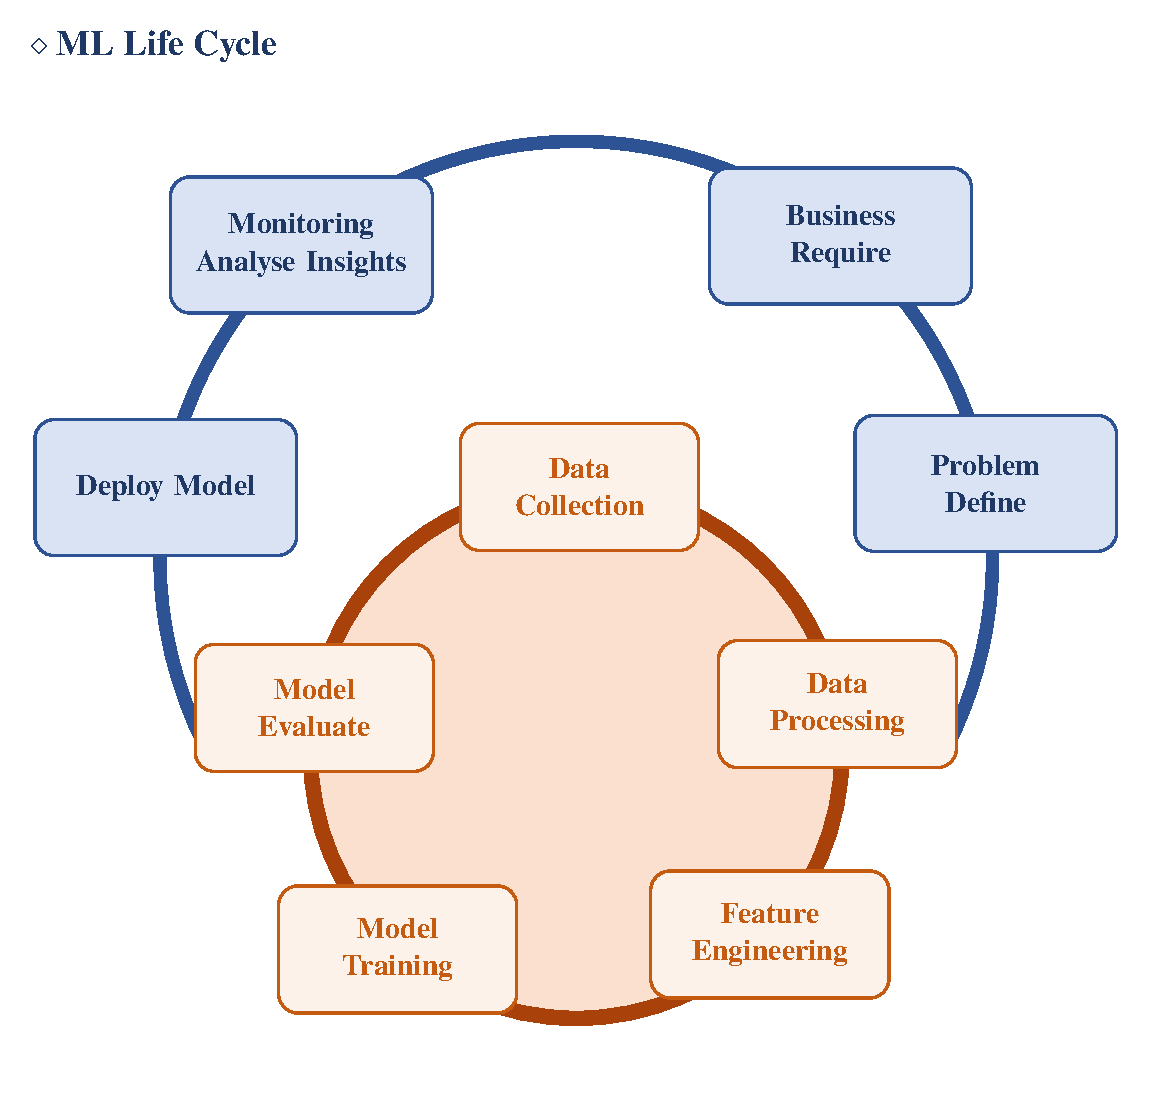
\includegraphics[width=0.68\textwidth]{sodo_ml_lifecycle_en.pdf}
    \caption[Vòng đời học máy, bản nhãn gốc tiếng Anh]{Vòng đời học máy, giữ nguyên nhãn
    tiếng Anh của tài liệu gốc. Nguồn: \textit{Data Version Control}~\cite{aivietnam2025dvc}.}
    \label{fig:ml_lifecycle_en}
\end{figure}


% ====================================================================
%  TÀI LIỆU THAM KHẢO
% ====================================================================
\chapter*{Tài liệu Tham khảo}
\addcontentsline{toc}{chapter}{Tài liệu Tham khảo}
\label{chap:thamkhao}

\begin{enumerate}[label={[\arabic*]}, noitemsep]
    \item Box, G. E. P., Jenkins, G. M., Reinsel, G. C., \& Ljung, G. M. (2015). \textit{Time Series Analysis: Forecasting and Control}. 5th ed. Wiley.
    \item Taylor, S. J., \& Letham, B. (2018). Forecasting at Scale. \textit{The American Statistician}, 72(1), 37--45.
    \item Breiman, L. (2001). Random Forests. \textit{Machine Learning}, 45(1), 5--32.
    \item Chen, T., \& Guestrin, C. (2016). XGBoost: A Scalable Tree Boosting System. \textit{Proceedings of KDD 2016}, 785--794.
    \item Hochreiter, S., \& Schmidhuber, J. (1997). Long Short-Term Memory. \textit{Neural Computation}, 9(8), 1735--1780.
    \item Vaswani, A., et al. (2017). Attention Is All You Need. \textit{Proceedings of NeurIPS 2017}, 5998--6008.
    \item Kimball, R., \& Ross, M. (2013). \textit{The Data Warehouse Toolkit}. 3rd ed. Wiley.
    \item NASA POWER Project. (2024). \url{https://power.larc.nasa.gov/}.
    \item Supabase Documentation. (2024). \url{https://supabase.com/docs}.
    \item IEA -- International Energy Agency. (2024). \url{https://www.iea.org/reports/renewables-2024}.
    \item Chandola, V., Banerjee, A., \& Kumar, V. (2009). Anomaly Detection: A Survey. \textit{ACM Computing Surveys}, 41(3), Article 15.
    \item Tukey, J. W. (1977). \textit{Exploratory Data Analysis}. Addison-Wesley.
\end{enumerate}

\end{document}
